\documentclass[10pt,polish,a4paper,oneside]{ppfcmthesis}

\usepackage[utf8]{inputenc}
\usepackage[OT4]{fontenc}



\usepackage[widespace]{fourier}   % Use Utopia font set
\usepackage[scaled=0.875]{helvet} % Use Helvetica for sans-serif
\renewcommand{\ttdefault}{lmtt}   % Use Lucida Mono for monotype
\usepackage{booktabs}             % Booktabs for tables
\usepackage{multirow}
\usepackage{algorithm2e}
\usepackage{placeins}
\renewcommand{\listalgorithmcfname}{Lista algorytmów}
\renewcommand{\algorithmcfname}{Algorytm}

\newcommand{\SA}[1]{$\mathit{SA}_{#1}$}
\newcommand{\ISA}[1]{$\mathit{ISA}_{#1}$}
\DeclareMathAlphabet{\mathcal}{OMS}{cmsy}{m}{n}
\newcommand{\bigO}[0]{\mathcal{O}}
\newcommand{\dollar}[0]{\$}

\author{Michał Nowak}

\title{Przegląd i~porównanie metod tworzenia tablic sufiksów oraz~ich~efektywna~implementacja~w~języku~Java}

\ppsupervisor{dr~inż.~Dawid Weiss}
\ppyear{2009}      % Year of final submission (not graduation!)

\begin{document}
% Front matter starts here
\frontmatter\pagestyle{empty}%
\maketitle\cleardoublepage%

% Blank info page for "karta dyplomowa"
\thispagestyle{empty}\vspace*{\fill}%
\begin{center}Tutaj przychodzi karta pracy dyplomowej;\\oryginał wstawiamy do wersji dla archiwum PP, w pozostałych kopiach wstawiamy ksero.\end{center}%
\vfill\cleardoublepage%

% Table of contents.
\pagenumbering{Roman}\pagestyle{ppfcmthesis}%
\tableofcontents* \cleardoublepage%

% Main content of your thesis starts here.
\mainmatter%

\chapter{Wstęp}

Wstęp\footnote{Treść przykładowych rozdziałów została skopiowana
z ,,zasad'' redakcji prac dyplomowych FCMu~\cite{fcm-red}.} do pracy powinien zawierać następujące elementy:
\begin{itemize}
    \item krótkie uzasadnienie podjęcia tematu; 
    \item cel pracy (patrz niżej); 
    \item zakres (przedmiotowy, podmiotowy, czasowy) wyjaśniający, w jakim rozmiarze praca będzie realizowana; 
    \item ewentualne hipotezy, które autor zamierza sprawdzić lub udowodnić; 
    \item krótką charakterystykę źródeł, zwłaszcza literaturowych; 
    \item układ pracy (patrz niżej), czyli zwięzłą charakterystykę zawartości poszczególnych rozdziałów; 
    \item ewentualne uwagi dotyczące realizacji tematu pracy np.~trudności, które pojawiły się w trakcie 
    realizacji poszczególnych zadań, uwagi dotyczące wykorzystywanego sprzętu, współpraca z firmami zewnętrznymi. 
\end{itemize}

\noindent
\textbf{Wstęp do pracy musi się kończyć dwoma następującymi akapitami:}
\begin{quote}
Celem pracy jest opracowanie / wykonanie analizy / zaprojektowanie / ...........
\end{quote}
oraz:
\begin{quote}
Struktura pracy jest następująca. W rozdziale 2 przedstawiono przegląd literatury na temat ........ 
Rozdział 3 jest poświęcony ....... (kilka zdań). 
Rozdział 4 zawiera ..... (kilka zdań) ............ itd. 
Rozdział X stanowi podsumowanie pracy. 
\end{quote}

W przypadku prac inżynierskich zespołowych lub magisterskich 2-osobowych, po tych dwóch w/w akapitach 
musi w pracy znaleźć się akapit, w którym będzie opisany udział w pracy poszczególnych członków zespołu. Na przykład:

\begin{quote}
Jan Kowalski w ramach niniejszej pracy wykonał projekt tego i tego, opracował ......
Grzegorz Brzęczyszczykiewicz wykonał ......, itd. 
\end{quote}


\chapter{Podstawy teoretyczne}


\section{Podstawowe pojęcia}

Niech $\Sigma$ oznacza skończony zbiór o~rozmiarze $|\Sigma| \geq 1$, zwany
dalej alfabetem \cite{taxonomy}. Elementami tego zbioru są symbole (w przypadku tekstu
zwykle utożsamiane z~pojedynczymi literami lub znakami). Alfabet określa się
jako indeksowalny, jeżeli istnieje permutacja indeksów taka, że 
$\forall_{i=0..|\Sigma|-1}: a_0 < a_1 < \dots < a_{|\Sigma|-1}$
(symbole mogą być uporządkowane).

Niech $x$ oznacza ciąg symboli (pojęcia symbol, znak i~litera będą
stosowane zamiennie) o~długości $n$.
Element ciągu $x$ występujący na pozycji $i$ oznacza się jako $x[i]$, $i \in
\langle0, n-1\rangle$. 
Przez $x[a..b]$, $0 \leq a \leq b \leq n-1$ rozumie się
podciąg $x$ rozpoczynający się na pozycji $a$, a~kończący na pozycji $b$ \cite{gusfield}.
Warto zauważyć, że $x = x[0..n-1]$.

\definicja{Prefiks} to taki podciąg $x$, którego pierwszy element
jest jednocześnie pierwszym elementem ciągu $x$, tj.~$x[0..b]$, $0 \leq b \leq
n-1$. 
\definicja{Sufiks} oznacza taki podciąg $x$, którego ostatni element jest
ostatnim znakiem ciągu $x$, tj. $x[a..n-1], 0 \leq a \leq n-1$. Przez
$S^{x}_{i}$ (lub $S_i$ w~przypadku braku niejednoznaczności) rozumie się
sufiks $x[i..n-1]$. Ciąg $x$ jest jednocześnie swoim najdłuższym prefiksem jak i~sufiksem \cite{gusfield}.

\definicja{Konkatenacją} dwóch ciągów $x$ i~$y$ o długości $n$ i~$m$ nazwiemy
ciąg $z$, dla którego $z = x \circ y = x[0] x[1] .. x[n-1] y[0] y[1] .. y[m-1]$. 


\section{Struktury danych}
    
\definicja{Drzewo trie} (\english{trie}) \cite{larsson99structures} jest typem
drzewa przeszukiwań, w~którym węzłom nie odpowiadają klucze, lecz ich fragmenty. W~dalszej
części pracy rozpatrywane będą drzewa, których kluczami są ciągi
symboli z~pewnego alfabetu.\footnote{W nomenklaturze polskiej zarówno 
\emph{tree}, jak i~\emph{trie} nazywane są drzewami~\cite{pknuthv3}, str.~528.
O~ile nie będzie powiedziane inaczej, przez drzewo będziemy
rozumieli drzewo \emph{trie}.} W~tego typu drzewach
krawędzie etykietowane są symbolami tego alfabetu, a~,,wartość'' klucza danego węzła wynika z~jego
pozycji i~jest konkatenacją etykiet krawędzi leżących na ścieżce prowadzącej
od korzenia drzewa do tego węzła. Wszystkie podwęzły danego
węzła mają wspólny prefiks równy wartości klucza ich rodzica.       
Nieco inny wariant takiego drzewa, nazwany \definicja{drzewem skompresowanym}
(\english{radix tree, Patricia trie}) \cite{larsson99structures}, polega na tym, że węzły
posiadające tylko jednego potomka są z~nimi łączone, a~symbole z~usuniętych
krawędzi są konkatenowane (zob.~rys.~\ref{rys:tree}). 

\begin{figure}[t]
    \begin{center}
       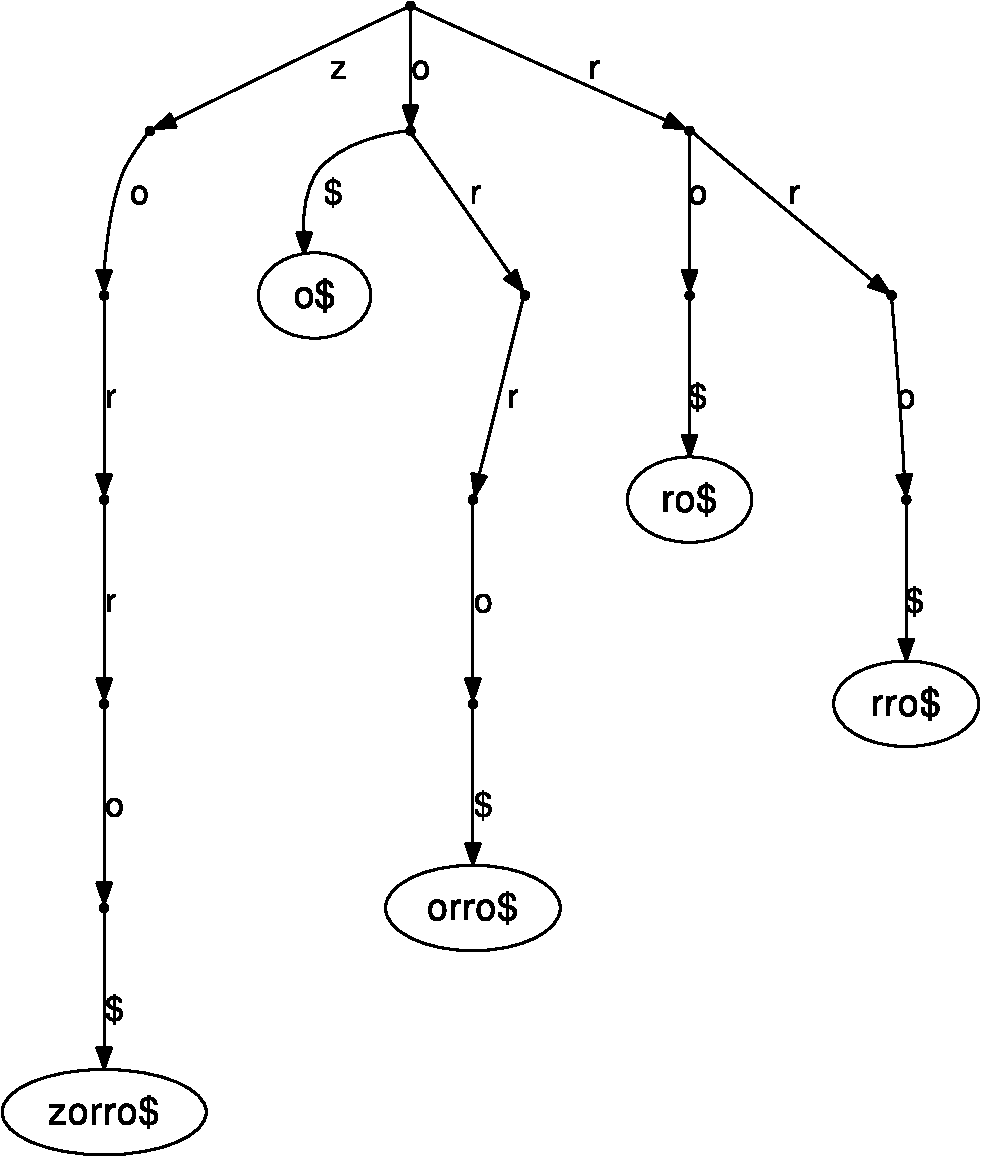
\includegraphics[scale=0.5]{figures/zorroSTrie.pdf}
    \end{center}

    \caption{Drzewo \emph{trie} dla zbioru sufiksów wyrazu ,,zorro'' z~dodanym unikalnym
    symbolem końcowym $\dollar$. Dla
    przejrzystości pominięto łuk od korzenia do liścia o~wartości $\dollar$.}%
    \label{rys:tree}
\end{figure}

\definicja{Drzewo sufiksów} (\english{suffix tree}) \cite{gusfield} dla ciągu symboli
$x$ z~alfabetu $\Sigma$ jest skompresowanym drzewem zbudowanym na zbiorze wszystkich sufiksów
$x$ o~następujących cechach:
\begin{itemize}
  \item krawędzie są etykietowane niepustymi ciągami symboli,
  \item każdy sufiks jest reprezentowany w~drzewie jako ścieżka od korzenia
  do liścia,
  \item wszystkie węzły wewnętrzne drzewa posiadają co najmniej dwóch
  potomków.
\end{itemize}

Zwyczajowo na końcu ciągu $x$ umieszczany jest znak specjalny $\dollar$,
leksykograficznie mniejszy od wszystkich symboli z~alfabetu $\Sigma$. Dzięki temu zabiegowi
żaden sufiks ciągu $x$ nie będzie prefiksem innego sufiksu, co zapewnia zachowanie wszystkich wyżej
wymienionych własności (w przeciwnym przypadku sufiksy mogłyby kończyć się
w~węzłach wewnętrznych drzewa). Rysunek \ref{rys:suffix-tree} prezentuje
drzewo sufiksów dla sekwencji ,,zorro\$''. Trzy ,,klasyczne'' algorytmy
tworzenia drzew sufiksów omówione zostały w~publikacjach \cite{weiner}, \cite{mccreight} 
i~\cite{ukkonen}. Ich porównanie można znaleźć w~pracy \cite{from-ukkonen}.

\begin{figure}[t]
    \begin{center}
        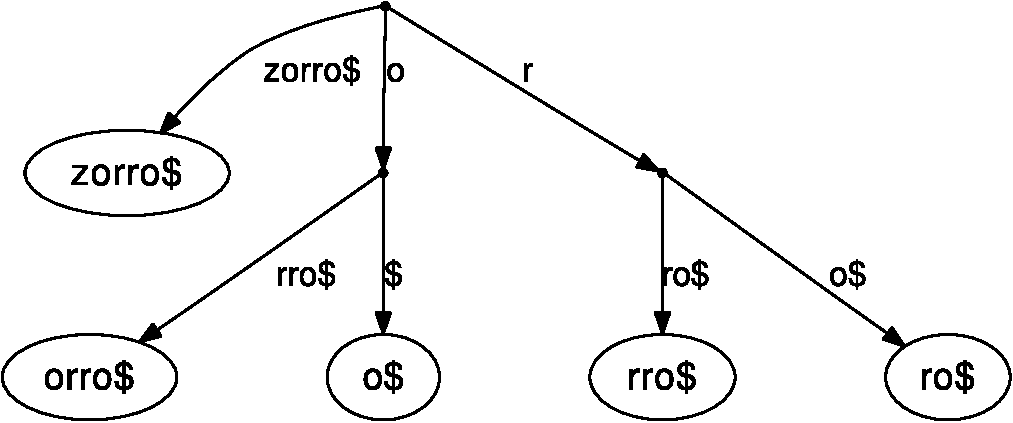
\includegraphics[scale=0.5]{figures/zorroST.pdf}
    \end{center}
    \caption{Drzewo sufiksów wyrazu ,,zorro\$''. Dla przejrzystości pominięto łuk od korzenia do
    liścia o~wartości $\dollar$.}%
    \label{rys:suffix-tree}
\end{figure}

W~literaturze powszechne jest etykietowanie sufiksów pozycją
ich pierwszego symbolu w~słowie $x$ -- przez sufiks o~etykiecie i~rozumie
się podciąg $x[i..n-1]$. \definicja{Tablica sufiksów} (\english{suffix
array}) \cite{taxonomy} słowa $x$~jest tablicą etykiet sufiksów uporządkowaną rosnąco według porządku
leksykograficznego sufiksów.
Tablicę sufiksów słowa $x$ oznacza się $\textit{SA}_x$ lub $\textit{SA}$ jeżeli pominięcie
identyfikatora słowa nie wprowadza niejednoznaczności. Formalnie,
$\textit{SA}[j] = i \iff x[i..n-1]$ jest $j$-tym sufiksem
słowa $x$ według porządku leksykograficznego. Warto zauważyć, że
$\textit{SA}$ jest zawsze permutacją liczb $0..n-1$. Rysunki
\ref{rys:suffix-array-vis} oraz \ref{rys:suffix-array}
prezentują tablicę sufiksów sekwencji symboli ,,zorro\$''.

\begin{figure}[t]
    \begin{center}
        \begin{tabular}{ c c l }
            \toprule
            $j$ & $\textit{SA}[j]=i$ & $x[i..n-1]$ \\
            \midrule
            0 & 5 &        $\dollar$ \\
            1 & 4 &        o$\dollar$ \\
            2 & 1 &        orro$\dollar$ \\
            3 & 3 &        ro$\dollar$ \\
            4 & 2 &        rro$\dollar$ \\
            5 & 0 &        zorro$\dollar$ \\
            \bottomrule
        \end{tabular}
    \end{center}
\caption{Tablica sufiksów dla sufiksów ciągu ,,zorro\dollar''.}%
\label{rys:suffix-array-vis}
\end{figure}

Dla tablicy sufiksów można zbudować \definicja{tablicę najdłuższych wspólnych podciągów}
(\english{longest common prefix array}) \cite{taxonomy} o~długości $n$, której elementy
$\textit{lcp}[i], i = 1..n-1$ oznaczają długość najdłuższego wspólnego prefiksu sufiksów
$\textit{SA}[i]$ i~$\mathit{SA}[i-1]$. Przykładowa tablica najdłuższych wspólnych prefiksów
zaprezentowana jest na rysunku \ref{rys:suffix-array}. Tablicę $\textit{lcp}$ można obliczyć
w~czasie liniowym znając \SA{} zgodnie z~metodami omówionymi w~artykułach \cite{lcp-kasai}
i~\cite{lcp-manzini}.

Strukturą komplementarną do tablicy sufiksów $\textit{SA}$ jest \definicja{odwrotna tablica
sufiksów} (\english{inverse suffix array}) \cite{taxonomy} oznaczana jako $\textit{ISA}$. Jest ona
permutacją liczb $0..n-1$ spełniającą zależność: $\textit{ISA}[i] = j \iff \textit{SA}[j] = i$.
Przykład odwrotnej tablicy sufiksów znajduje się na rysunku \ref{rys:suffix-array}. Wartość $k$-tego
wpisu w~tablicy \SA{} oznacza identyfikator sufiksu na $k$-tej pozycji w~porządku leksykograficznym;
$k$-ty wpis w~tablicy \ISA{} oznacza pozycję sufiksu $k$ w~tablicy \SA{} (oraz w~porządku
leksykograficznym).    

\begin{figure}[t]
    \begin{center}        
        \begin{tabular}{ r c c c c c c l}                           
                           & 0 & 1 & 2 & 3 & 4 &  5   &   \\ \cmidrule{2-7}
                   $x = [$ & z & o & r & r & o & $\dollar$ & ] \\ 
         $\mathit{SA} = [$ & 5 & 4 & 1 & 3 & 2 &  0   & ] \\ 
        $\mathit{ISA} = [$ & 5 & 2 & 4 & 3 & 1 &  0   & ] \\ 
        $\mathit{lcp} = [$ & - & 0 & 1 & 0 & 1 &  0   & ] \\ 
        \end{tabular}            
    \end{center}                         
\caption{Tablica sufiksów $\mathit{SA}$, odwrotna tablica sufiksów $\mathit{ISA}$
oraz tablica najdłuższych prefiksów $\mathit{lcp}$ dla sekwencji
,,zorro\dollar''.}%
\label{rys:suffix-array}
\end{figure}
    
Przez \definicja{h-grupę} (\english{h-group}) \cite{taxonomy} rozumie się podzbiór
sufiksów słowa $x$ o~wspólnym prefiksie długości $h>0$. 
Podział sufiksów na \emph{h-grupy} otrzymuje się poprzez ich częściowe
uporządkowanie ze względu na wartość $h$~pierwszych symboli sufiksu.
Proces ten nosi nazwę \emph{h-sortowania} (\english{h-sort}), w~jego
wyniku sufiksy uporządkowane są według \emph{h-porządku}
(\english{h-order}). Sufiksy należące do jednej \emph{h-grupy} są sobie
równe pod względem \emph{h-porządku}. Algorytmy \emph{h-sortowania}
są zazwyczaj stabilne, czyli zachowują wcześniejszy porządek sufiksów.
Każdej \emph{h-grupie} można przypisać pewien identyfikator
(\english{h-rank}). W~zależności od potrzeb algorytmu, wartości
identyfikatorów dobierane są na jeden z~trzech sposobów:
\begin{enumerate}
  \item grupa identyfikowana jest pozycją pierwszego jej elementu w~przybliżonej tablicy sufiksów -- głowa (\english{head}) grupy,
  \item grupa identyfikowana jest pozycją ostatniego elementu w~przybliżonej
   tablicy sufiksów -- ogon (\english{tail}) grupy,
  \item  każdej z~\emph{h-grup} (nawet jednoelementowym) przypisywane są
  rosnące identyfikatory zgodnie z~kolejnością ich pojawienia się w~$\textit{SA}_h$.
\end{enumerate}

\noindent
Wyniki \emph{h-sortowania} zachowuje się w~\definicja{przybliżonej
tablicy sufiksów} (\english{approximate suffix array}) \cite{taxonomy} oznaczanej
$\textit{SA}_h$. Możliwe jest również wyznaczenie
\definicja{przybliżonej odwrotnej tablicy sufiksów}
(\english{approximate inverse suffix array}) \cite{taxonomy} $\textit{ISA}_h$.
$\textit{SA}_h$ jest permutacją liczb $0..n-1$, natomiast
$\textit{ISA}_h$ może zawierać wartości powtarzające się. Wynika to z~tego,
że każdemu sufiksowi należącemu do danej \emph{h-grupy} przypisywany jest jej identyfikator.
Przykład przybliżonej tablicy sufiksów znajduje się na rysunku \ref{rys:approx-suffix-array}.

\begin{figure}[t]
    \begin{center}        
        \begin{tabular}{ r c c c c c c c c c c c c l}                           
                                 & 0  & 1  & 2  & 3 & 4 & 5   & 6  & 7  & 8 & 9  & 10 & 11     \\ \cmidrule{2-13} 
                         $x = [$ & a  & b  & e  & a & c & a   & d  & a  & b & e  & a  &
                       $\dollar$ &]\\ $\mathit{SA}_1 = [$ & 11 & (0 & 3  & 5 & 7 & 10) & (1 & 8) & 4 & 6  & (3 & 9)   & ] \\ 
            $\mathit{ISA}_1 = [$ & 1  & 6  & 10 & 1 & 8 & 1   & 9  & 1  & 6 & 10 & 1  & 0    & ]\\
                           lub [ & 5  & 7  & 11 & 5 & 8 & 5   & 9  & 5  & 7 & 11 & 5  & 0    & ]\\
                           lub [ & 1  & 3  & 5  & 1 & 3 & 1   & 4  & 1  & 2 & 5  & 1  & 0    & ]\\
        \end{tabular}            
    \end{center}                         
\caption{Przykłady przybliżonej tablicy sufiksów oraz przybliżonej 
odwrotnej tablicy sufiksów dla $h=1$. \emph{H-grupy}
wyróżnione zostały nawiasami. Na rysunku przedstawione są 3 wersje tablicy
$\textit{ISA}_1$ różniące się metodami przypisywania identyfikatorów grupom 
(wypisane w~kolejności przedstawienia w~tekście).  Źródło: \cite{taxonomy}.}%
\label{rys:approx-suffix-array}
\end{figure}

W~niektórych publikacjach przyjęto inną konwencję nazewniczą, \emph{h-grupa} nazywana
jest tam \emph{h-kubełkiem} lub po prostu \emph{kubełkiem} (\english{bucket}).
Tablica $\textit{ISA}_h$ nazywana jest \definicja{tablicą wskaźników na kubełki} 
(\english{bucket pointer array}) \cite{schurmann-phd}.

\chapter{Podział metod tworzenia tablic sufiksów}

Tablice sufiksów zostały przedstawione w~roku 1990 przez Udiego Manbera i~Gene'a
Mayersa wraz z~pierwszym algorytmem ich tworzenia \cite{Manber90}.
Zestawienie ważniejszych algorytmów tworzenia tablic sufiksów
znajduje się w~tabeli \ref{tab:alg}. Autorzy pracy \cite{taxonomy} podsumowują
obecny stan wiedzy na temat tworzenia tablic sufiksów w~trzech punktach:
\begin{itemize}
  \item istnieją algorytmy efektywne pamięciowo o~złożoności liniowo zależnej
  od długości wejścia, np. \emph{smaller-larger}, \emph{skew},
  \item istnieją algorytmy szybsze w~praktycznych zastosowaniach pomimo swojej
  nieliniowej pesymistycznej złożoności, np. \emph{bpr}, \emph{improved  two-stage}, \emph{deep shallow}.
  \item każdy problem, którego rozwiązanie można znaleźć z~pomocą drzew sufiksów
  może zostać rozwiązany w~tym samym czasie przy pomocy tablic sufiksów
  \cite{replacing}.
\end{itemize}

\noindent
Niezrealizowanym do tej pory celem jest zaprojektowanie takiego algorytmu
tworzenia tablic sufiksów, który (za \cite{taxonomy}):
\begin{itemize}
  \item posiada minimalną złożoność asymptotyczną $\Theta(n)$,
  \item  jest szybki \emph{w~praktyce}, to znaczy na dużych rzeczywistych
  zbiorach danych, np. [\ref{hart}],
  \item jest \emph{lekki} -- wymaga niewiele więcej pamięci ponad ilość
  potrzebną do przechowania $x$ i~\SA{x}.
\end{itemize}


\noindent 
Autorzy prac \cite{taxonomy} oraz \cite{schurmann-phd} podjęli próbę stworzenia taksonomii
metod tworzenia tablic sufiksów. Proponowane przez nich metody są do siebie bardzo podobne,
a~klasyfikacja proponowana przez \cite{taxonomy} została rozbudowana w~pracy \cite{schurmann-phd}.
  
W~dalszej części pracy omówiona zostanie klasyfikacja proponowana przez Klausa-Bernda Schürmanna
\cite{schurmann-phd} poszerzona o~algorytm \emph{improved two-stage}.

\begin{table}[t]
	\begin{center}        
    \begin{tabular}{l c c c }
    \toprule
    Algorytm                  &           Publikacja            &    Złożoność obliczeniowa    & Złożoność pamięciowa \\ \midrule
    \emph{bpr}                &      \cite{schurmann-phd}       & $\bigO (\frac{n^2}{\log n})$ &       $9-10n$        \\         
    \emph{cache}              &          \cite{seward}          &     $\bigO(n^2 \log n)$      &         $9n$         \\         
    \emph{copy}               &          \cite{seward}          &     $\bigO(n^2 \log n)$      &         $5n$         \\         
    \emph{deep shallow}       &            \cite{MF}            &     $\bigO(n^2 \log n)$      &         $5n$         \\         
    \emph{difference-cover}   &      \cite{Burkhardt2003}       &      $\bigO(n \log n)$       &        $5-6n$        \\         
    \emph{improved two-stage} &            \cite{MP}            &     $\bigO(n^2 \log n)$      &         $5n$         \\         
    \emph{odd-even}           & \cite{kim} i~\cite{kim-jo-park} &    $\bigO(n \log \log n)$    &          --          \\         
    \emph{prefix-doubling}    &         \cite{Manber90}         &       $\bigO(n\log n)$       &         $8n$         \\         
    \emph{qsufsort}           &            \cite{LS}            &       $\bigO(n\log n)$       &         $8n$         \\         
    \emph{skew}               &            \cite{KS}            &          $\bigO(n)$          &       $10-13n$       \\         
    \emph{smaller-larger}     &          \cite{Ko2005}          &          $\bigO(n)$          &       $7-10n$        \\         
    \emph{two-stage}          &            \cite{IT}            &     $\bigO(n^2 \log n)$      &         $5n$         \\         
    \bottomrule
    \end{tabular}
    \end{center}                         
    \caption{Zestawienie ważniejszych metod tworzenia tablic sufiksów.
    Złożoność pamięciowa podana jest dla sytuacji, gdy jeden symbol zajmuje 1
    jednostkę pamięci a~jedna liczba -- 4 jednostki pamięci. Źródło: opracowanie
    własne na podstawie \cite{taxonomy} i~\cite{schurmann-phd}.}%
    \label{tab:alg}
\end{table}


\section{Podział metod ze względu na proces sortowania sufiksów}

W~pracy \cite{schurmann-phd} zaproponowano dwa ortogonalne typy klasyfikacji
algorytmów: pierwszy z~nich dzieli algorytmy ze względu na przebieg procesu
sortowania sufiksów; drugi ze
względu na sposób wykorzystania zależności między sufiksami. Podział
algorytmów według obu typów klasyfikacji przedstawiony jest w~tabeli
\ref{tab:schurmann}.

Klasyfikacja algorytmów ze względu na proces sortowania sufiksów opiera się na
odpowiedzi na pytanie: ,,które sufiksy są przetwarzane w~pierwszej kolejności
i~jak przebiega dalej proces sortowania?''. Algorytmy dzielone są następnie na 
dwie podgrupy: wykorzystujące \definicja{polepszanie kubełków} (\english{bucket
refinement}) oraz \definicja{sortowanie zredukowanych ciągów znaków} (\english{reduced string sorting}).


\subsection{Polepszanie kubełków}

Pod pojęciem polepszania kubełków kryje się utworzenie \emph{k-porządku}
sufiksów na podstawie wyliczonego wcześniej \emph{h-porządku} sufiksów ($k>h$).

Pierwszy typ algorytmów wykorzystujących polepszanie kubełków opiera się na ogólnych metodach
sortowania ciągów znaków (które nie wykorzystują wiedzy o~zależnościach między sufiksami). Algorytmy
tego typu wykonują \emph{h-sortowanie} dla zwiększającego się $h$ dopóki wszystkie \emph{h-grupy}
(kubełki) nie będą zawierały tylko jednego elementu. Algorytmy należące do tej kategorii to
\emph{MSD radix sort} omówiony w~pracy \cite{radix} i~\emph{multikey quicksort}
opisany~w~\cite{bentley}.

Drugi typ algorytmów polepszania kubełków opiera się na następującej obserwacji: jeżeli dwa sufiksy
słowa $x$ $x[u,n-1]$ i~$x[v,n-1]$ mają wspólny prefiks długości $\ell$, to ich porządek można
wywnioskować na podstawie porządku ich $\ell\textit{-następców}$ $x[u+\ell, n-1]$ i~$x[v+\ell, n-1]$
(przykładem tego procesu jest drugi etap algorytmu \emph{two-stage}). Algorytmy z~tej grupy można
podzielić na dwa dalsze podtypy:
\begin{itemize}
	\item algorytmy wykonujące \definicja{polepszanie wszerz}
	(\english{breadth-first refinement}). Metody te dokonują \emph{h-sortowania}
	ze zwiększającym się $h$~aż do uzyskania jednoelementowych kubełków
	(\emph{h-grup}). Do tej grupy algorytmów należą \emph{prefix-doubling} 
	\cite{Manber90} i~\emph{qsufsort} \cite{LS}.
	
	\item algorytmy wykonujące \definicja{polepszanie wgłąb} (\english{depth-first
	refinement}).
	Metody te wykorzystują następujący schemat polepszania kubełków: dla dowolnego
	$h$, sortowanie sufiksów kolejnego kubełka następuje dopiero po tym, gdy
	poprzedni kubełek jest w~pełni posortowany, czyli wszystkie jego podkubełki są
	jednoelementowe. Na przykład, dla ciągu ,,,AAABBABBBAAABBAB'' po
	\emph{1-sortowaniu} grupa sufiksów rozpoczynających się od symbolu $B$ będzie
	sortowana dopiero wtedy, gdy będzie ustalony porządek sufiksów
	rozpoczynających się od $A$; podczas sortowania tej grupy porządek sufiksów
	o~prefiksie ,,AB'' będzie ustalony dopiero po posortowaniu sufiksów rozpoczynających się od ,,AA'' itd.
	 Metody tego typu wykorzystują naiwne metody typu pierwszego w~sytuacji, 
	 gdy porządek $\ell\textit{-następców}$ jest jeszcze nieznany.
	 Do tej kategorii algorytmów należą między innymi: \emph{two-stage}, \emph{copy},
	  \emph{cache} oraz \emph{deep shallow}. W~ogólności metody tego typu są bardzo szybkie w~praktyce, pomimo ich wysokiej złożoności sięgającej nawet $\bigO(n^2\log n)$.
\end{itemize}

Rysunek \ref{rys:bucket-refinement} przedstawia etapy procesu polepszania
kubełków dla ciągu ,,AAABBABBBAAABBAB''. Każdy sufiks reprezentowany jest przez
pionową linię której wysokość oznacza jego pozycję według porządku
leksykograficznego: niska linia oznacza sufiks leksykograficznie mniejszy od
sufiksu reprezentowanego przez wyższą linię. Na rysunku
\ref{rys:bucket-refinement} widać (od góry): stan początkowy, stan w~trakcie
działania algorytmu (w przypadku polepszania wszerz jest to stan po
posortowaniu według prefiksu długości 2; dla polepszania wgłąb jest to stan po uporządkowaniu
sufiksów rozpoczynających się od symbolu ,,A''), stan końcowy -- posortowane sufiksy.

\begin{figure}[t]
    \begin{center}
        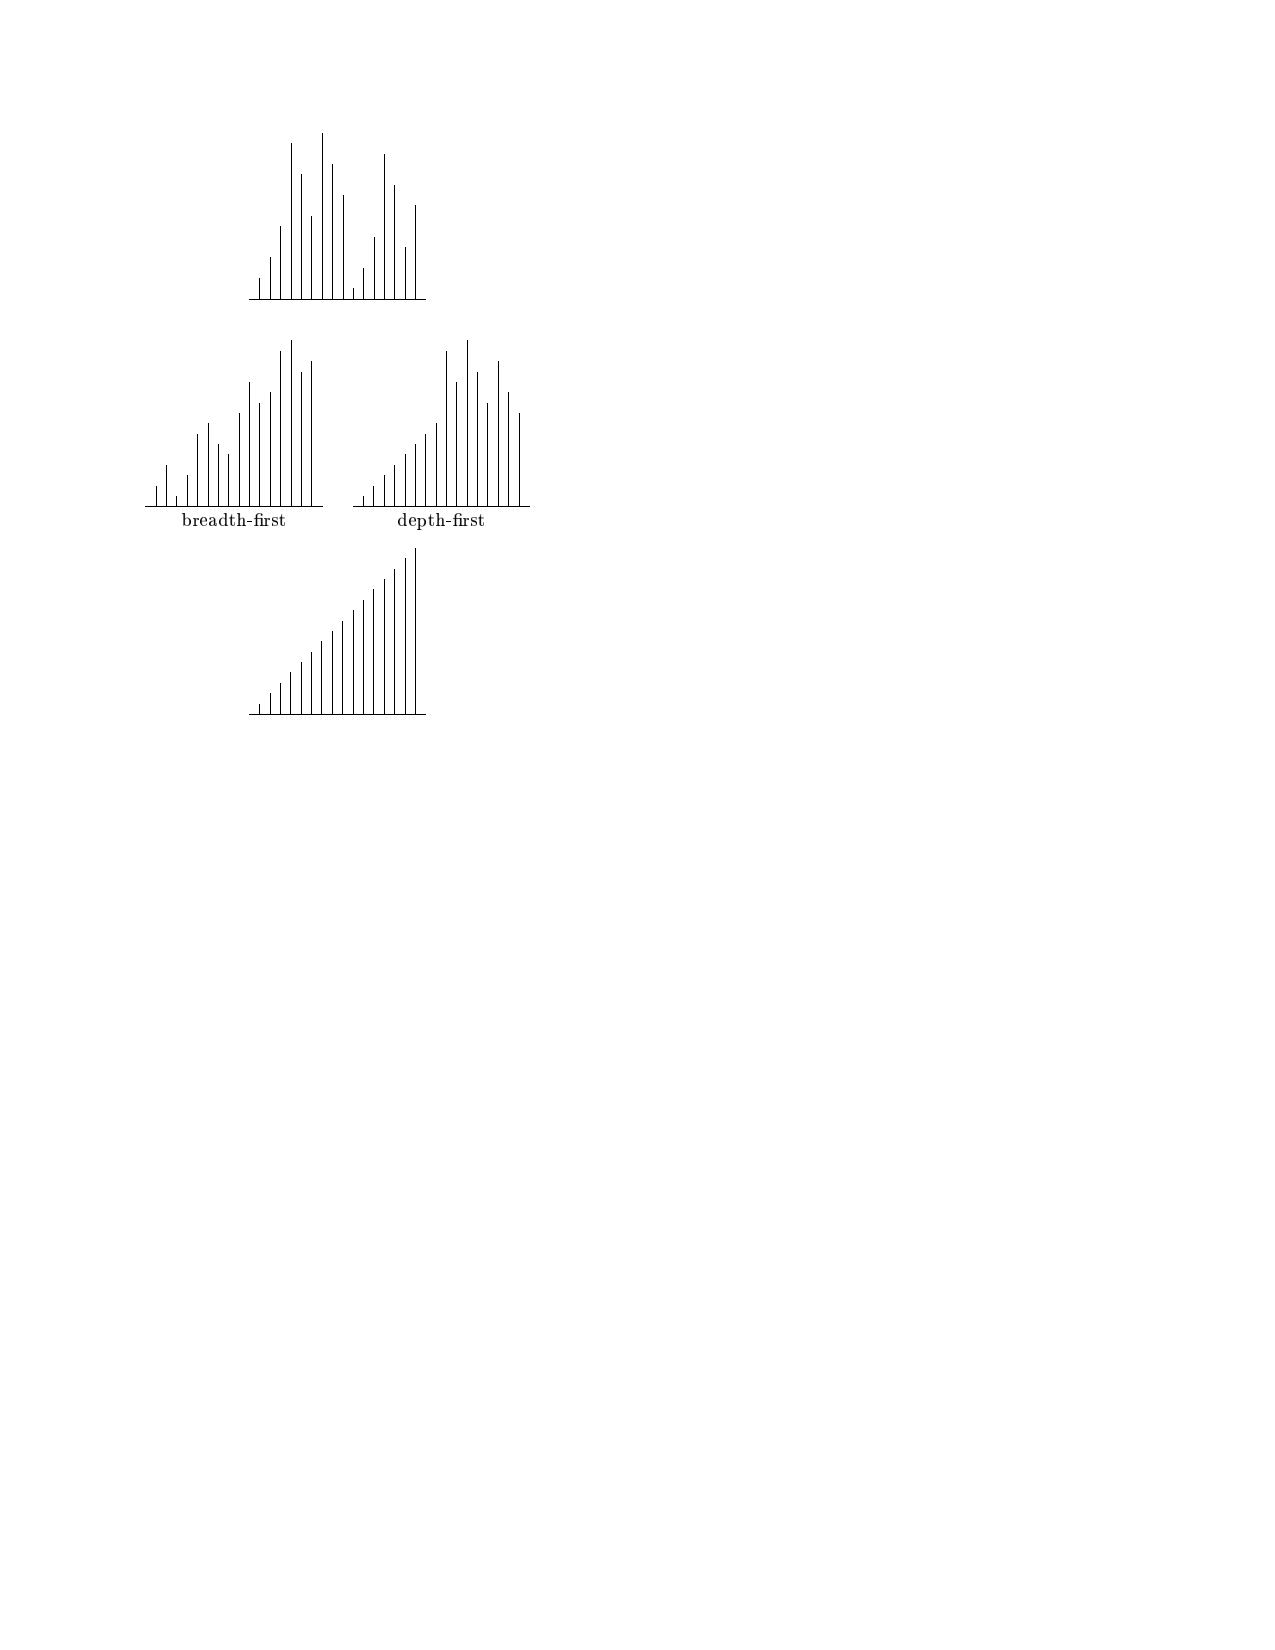
\includegraphics[scale=0.75]{figures/bucket-refinement.pdf}
    \end{center}        

    \caption{Etapy algorytmu polepszania kubełków dla wyrazu
    ,,AAABBABBBAAABBAB''. Źródło: \cite{schurmann-phd}.}%
    \label{rys:bucket-refinement}
\end{figure} 


\begin{table}[t]
	\begin{center}
    \begin{tabular}{l @{\hspace{2em}} c @{\hspace{2em}} c}
    \toprule
    Typ algorytmu            &     strategia \emph{push}             &    strategia \emph{pull}      \\
    \midrule
    Polepszanie wszerz       &        \emph{prefix-doubling}         &        \emph{qsufsort}        \\                                      
    \addlinespace[1em]
    Polepszanie wgłąb        &           \emph{two-stage}            &         \emph{cache}          \\                                      
                             &              \emph{copy}              &          \emph{bpr}           \\                                      
                             &          \emph{deep-shallow}          &                               \\                                      
                             &       \emph{improved two-stage}       &                               \\                                      
    \addlinespace[1em]
    Sortowanie zred.~ciągów znaków &        \emph{skew}              &    \emph{difference-cover}    \\                                      
                             &            \emph{odd-even}            &                               \\                                      
                             &         \emph{smaller-larger}         &                               \\                                      
    \bottomrule
    \end{tabular}
    \end{center}                         
    \caption{Podział algorytmów tworzenia tablic sufiksów według taksonomii
    zaproponowanej w~pracy \cite{schurmann-phd}. Źródło: opracowanie własne w~oparciu o~\cite{schurmann-phd}.}%
    \label{tab:schurmann}
\end{table}

\subsection{Sortowanie zredukowanych ciągów znaków}

Metody tego typu działają według następującego schematu: na początku wybierany jest podzbiór
\emph{sub} identyfikatorów sufiksów, odpowiadające im sufiksy są potem sortowane na podstawie
prefiksów ustalonej długości. Następnie każdemu z~tych sufiksów przypisywany jest pewien klucz
odpowiadający jego porządkowi wg. prefiksów. Następnie tworzony jest taki ciąg $t^{\textit{sub}}$
długości $|\textit{sub}|$ zawierający wcześniej przydzielone klucze, którego \SA{t^{\textit{sub}}}
odpowiada porządkowi leksykograficznemu sufiksów identyfikowanych zbiorem \emph{sub}. Tablica
\SA{t^{\textit{sub}}} może być obliczana rekurencyjnie tym samym algorytmem, lub z~wykorzystaniem
efektywnego algorytmu sortowania ciągów znaków (\cite{bentley-sort}, \cite{radix}, [\ref{ssort}],
\cite{bentley}, \cite{sinha}). W~pełni uporządkowane sufiksy ze zbioru \emph{sub} służą potem do
posortowania pozostałych sufiksów. Ostatecznie budowana jest pełna tablica sufiksów. Do algorytmów
realizujących powyższy schemat należą: \emph{difference-cover}, \emph{skew}, \emph{odd-even} oraz
\emph{smaller-larger}.

Rysunek \ref{rys:reduced-string-sorting} przedstawia etapy działania algorytmu
sortowania zredukowanych ciągów znaków. Podobnie jak na rysunku
\ref{rys:bucket-refinement}, sufiksy reprezentowane są przez pionowe linie,
których wysokość oznacza miejsce sufiksu w~porządku leksykograficznym. Sufiks
reprezentowany przez mniejszą linię jest leksykograficznie mniejszy od sufiksu
reprezentowanego przez wyższą linię. Na rysunku przedstawiono po kolei (od
góry): stan początkowy; stan algorytmu w~sytuacji gdy posortowane są sufiksy
o~nieparzystych identyfikatorach; stan końcowy.


\begin{figure}[t]
    \begin{center}
        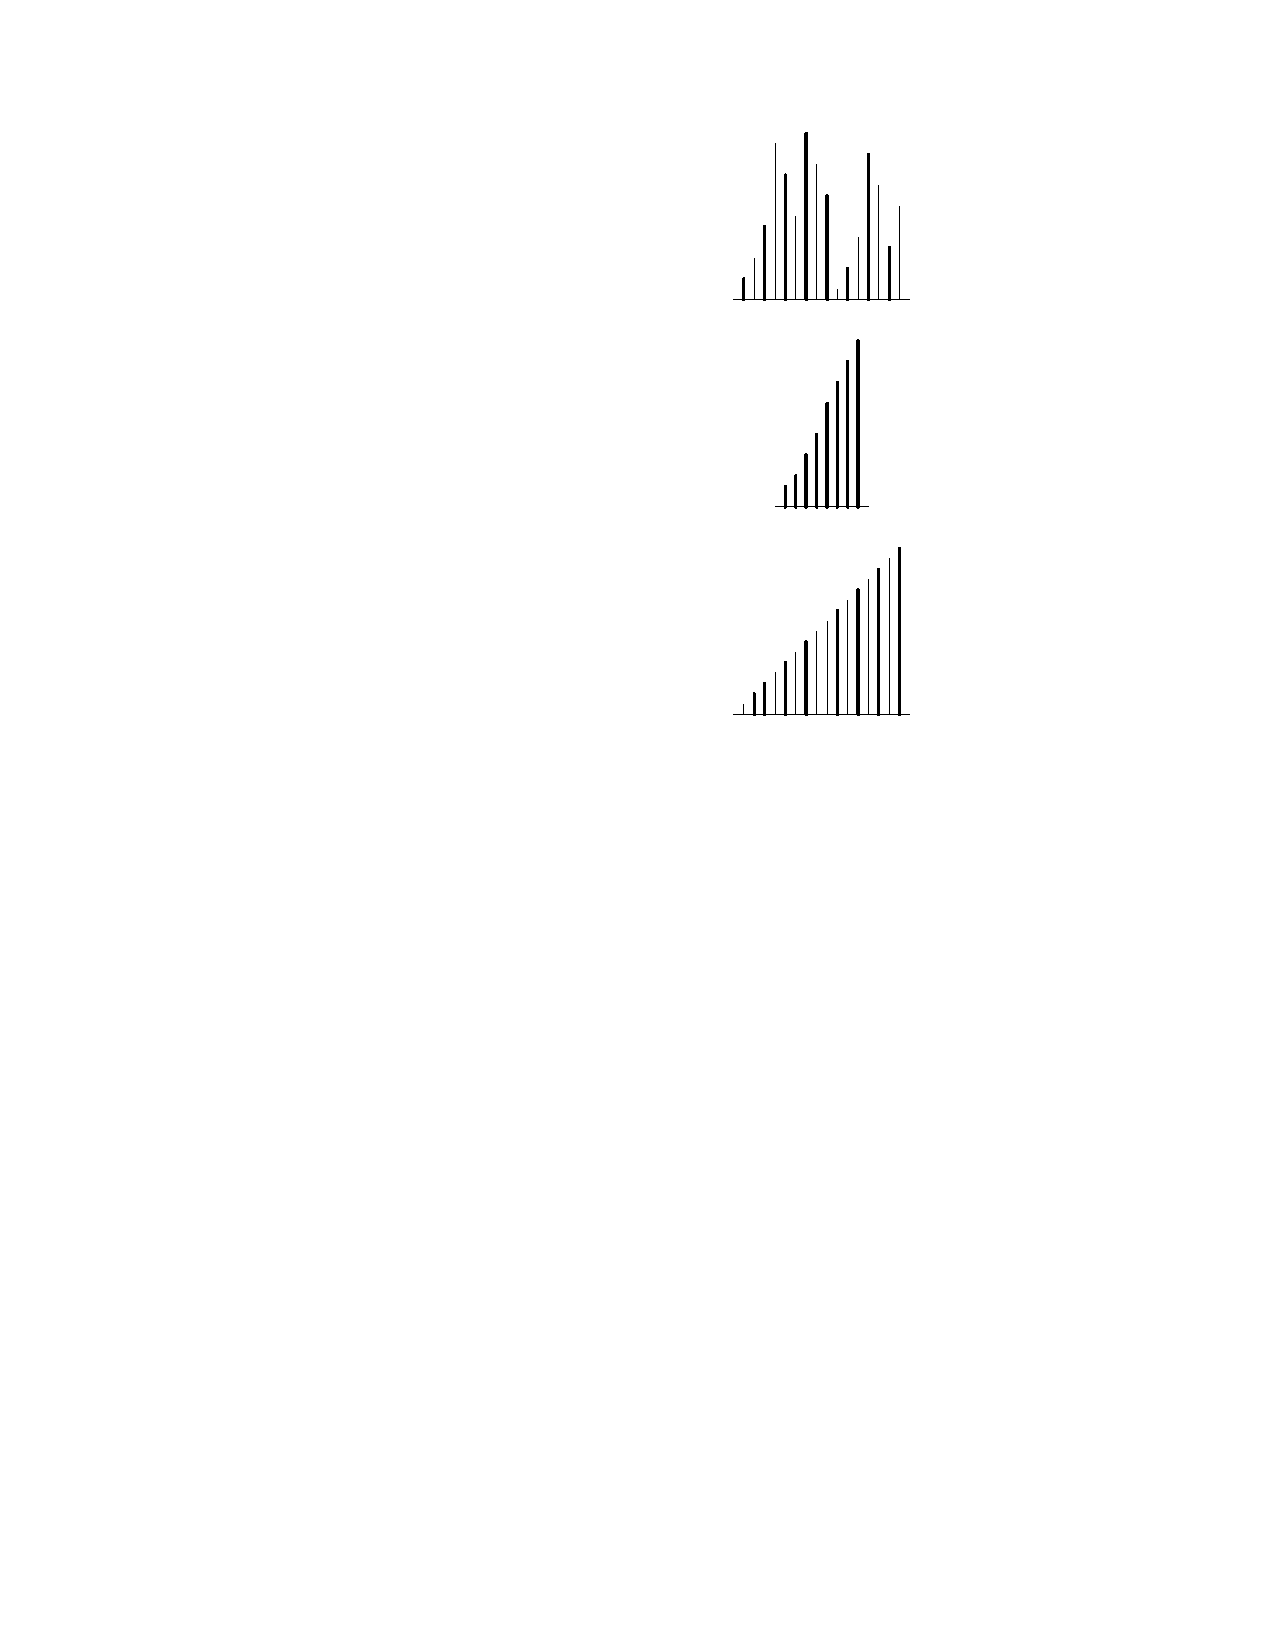
\includegraphics[scale=0.75]{figures/reduced-string-sorting.pdf}
    \end{center}        
    \caption{Etapy algorytmu sortowania zredukowanych ciągów znaków dla wyrazu
    ,,AAABBABBBAAABBAB''. Źródło: \cite{schurmann-phd}.}%
    \label{rys:reduced-string-sorting}
\end{figure} 

\section{Podział ze względu na sposób wykorzystania zależności między sufiksami}

Drugim sposobem podziału zaproponowanym w~pracy \cite{schurmann-phd} jest
podział algorytmów tworzenia tablic sufiksów ze względu na sposób wykorzystania
zależności między sufiksami. Jeżeli dwa sufiksy $x[u,n-1]$ i~$x[v,n-1]$ mają
wspólny prefiks długości $\ell$, to ich porządek można ustalić na podstawie
porządku sufiksów $x[u+\ell,n-1]$ i~$x[v+\ell,n-1]$. Rozróżnia się dwie metody
wykorzystywania tej zależności: metodę \emph{pull} i~metodę
\emph{push}.
Terminy \emph{pull} i~\emph{push} pochodzą z~terminologii systemów
informacyjnych, oznaczają różne strategie komunikacji pomiędzy nadawcą
wiadomości i~jej odbiorcą. Metoda \emph{push} oznacza sytuację, kiedy dostawca
wiadomości nawiązuje komunikację. Odwrotna sytuacja następuje w~strategii
\emph{pull} -- tutaj to odbiorca zgłasza żądanie inicjalizacji komunikacji.

W~odniesieniu do algorytmów tworzenia tablic sufiksów metoda \emph{push} polega na tym, że
wykorzystuje porządek wcześniej obliczonych grup sufiksów do ustalenia porządku grup sufiksów
$\ell$\textit{-poprze\-dni\-ków}, tzn. po ustaleniu porządku sufiksów $x[u+\ell,n-1]$ i~$x[v+\ell,n-1]$
obliczany jest porządek sufiksów $x[u,n-1]$ i~$x[v,n-1]$. Wzorcowym przykładem wykorzystania tej
techniki jest algorytm \emph{two-stage}.

Metoda \emph{pull} jest wykorzystywana w~procesie sortowania opierającego się o~porównania. Podczas
porównywania sufiksów $x[u,n-1]$ i~$x[v,n-1]$ sprawdzany jest porządek sufiksów $x[u+\ell,n-1]$
i~$x[v+\ell,n-1]$. Algorytm \emph{qsufsort} jest najlepszym przykładem zastosowania tej techniki.



\chapter{Wybrane metody tworzenia tablic sufiksów}

W~poniższym rozdziale omówione są wybrane metody tworzenia tablic sufiksów.
Algorytmy wybrane zostały na podstawie wyników testów wydajnościowych
zaprezentowanych w~pracach \cite{taxonomy} i~\cite{schurmann-phd} oraz
publikowanych na stronach [\ref{msufsort}] i~[\ref{mori-benchmark}].
Algorytmy uzyskujące dobre wyniki na dużych zbiorach danych -- szybkie \emph{w
praktyce} pochodzą z~rodziny algorytmów wykorzystujących \emph{polepszanie
wszerz}. W~poniższym zestawieniu opisane zostały również algorytmy
reprezentujące inne grupy metod tworzenia tablic sufiksów: \emph{polepszanie
wgłąb} i~\emph{sortowanie zredukowanych ciągów znaków}.


\section{Algorytm \emph{skew}}

Algorytm \emph{skew} został opracowany przez Petera Sandersa i~Juhę
K\"arkk\"ainena \cite{KS}. Dostępna jest
również implementacja tego algorytmu ich autorstwa [\ref{KScode}]. Opisywana
metoda pochodzi z~rodziny algorytmów wykorzystujących
\emph{sortowanie zredukowanych ciągów znaków}. 
Algorytm wykonuje 3 główne kroki:
\begin{enumerate}
  \item Tworzenie tablicy sufiksów zbudowanej z~sufiksów $S_i$ o~indeksach $i
  \bmod{3} \neq 0$. Problem jest redukowany do tworzenia tablicy sufiksów ciągu długości $2/3$ 
  rozmiaru ciągu wejściowego, a~następnie rozwiązywany rekurencyjne.
  \item Tworzenie tablicy sufiksów zbudowanej z~sufiksów pominiętych w~pierwszym kroku z~wykorzystaniem tablic sufiksów z~kroku 1.
  \item Połączenie zbudowanych tablic w~jedną.
\end{enumerate}

\noindent
Pierwszy (i najbardziej czasochłonny) krok algorytmu polega na posortowaniu
sufiksów $S_i$ dla $i \bmod{3} \neq 0$, czyli utworzeniu tablicy sufiksów
$\textit{SA}^{12}$. Jeżeli w~wyniku \emph{h-sortowania} dla $h=3$ wszystkie
grupy są jednoelementowe, to ten etap algorytmu się kończy. W~przeciwnym przypadku
każdemu sufiksowi $S_i$ nadawany jest identyfikator $x^{'}_i
\in [ 1, 2n/3]$ będący identyfikatorem jego \emph{3-grupy} powstałej po 
\emph{3-sortowaniu}. Następnie tworzony jest ciąg $x^{12} = [x^{'}_i : i
\bmod{3} = 1] \circ [x^{'}_i : i \bmod{3} = 2]$, którego tablica sufiksów
$\textit{SA}_{x^{12}}$ obliczana jest rekurencyjnie. Tablica $\textit{SA}^{12}$
wypełniana jest zgodnie z~poniższym wzorem ($n_1$ oznacza liczbę sufiksów o~etykietach $i$ takich, że $i \bmod{3} = 1$):  
\begin{displaymath}
\textit{SA}^{12}[i] = \left\{ 
    \begin{array}{l l}
    1 + 3k          & \textit{jeżeli } k = \textit{SA}_{x^{12}}[i] <  n_1, \\
    2 + 3(k - n_1)  & \textit{w przeciwnym wypadku}.
    \end{array} 
    \right.
\end{displaymath}

Drugi krok algorytmu polega na utworzeniu tablicy sufiksów $\textit{SA}^0$
złożonej z~sufiksów $S_i$, gdzie $i \bmod{3} = 0$. Tablica ta powstaje w~wyniku
sortowania par $(x[i], S_{i+1})$. Ponieważ porządek sufiksów $S_{i+1}$ jest
zawarty w~$\textit{SA}^{12}$, do znalezienia $\textit{SA}^0$ wystarczy posortować
stabilnie elementy $\textit{SA}^{12}[j]$ reprezentujące sufiksy
$\textit{SA}_{i+1}, i \bmod{3} = 0$ według wartości $x[i]$. Można tego dokonać
w~czasie liniowym jednym krokiem sortowania kubełkowego.

Trzeci krok algorytmu polega na połączeniu tablic $\textit{SA}^{12}$ i~$\textit{SA}^0$ w~jedną 
tablicę sufiksów. Porównywanie sufiksów $S_j$, gdzie $j\bmod{3}=0$ i~$S_i, i \bmod{3} \neq 0$ 
odbywa się na jeden z~dwóch sposobów:
\begin{itemize}
    \item Jeżeli $i \bmod{3} = 1$, to porządek sufiksów $S_i$ i~$S_j$ można
  ustalić porównując pary $(x[i], S_{i+1})$ oraz $(x[j], S_{j+1})$. Ponieważ $i+1
  \bmod{3} = 2$ i~$j+1 \bmod 3 = 1$ porządek sufiksów $S_{i+1}$ i~$S_{j+1}$
  można ustalić na podstawie ich pozycji w~$\textit{SA}_{x^{12}}$. Ta pozycja może
  być ustalana w~czasie stałym, jeżeli obliczona zostanie tablica
  $\textit{ISA}_{x^{12}}$.
  
    \item Analogicznie, jeżeli $i \bmod{3} =
  2$, to porównywane są trójki $(x[i], x[i+1], S_{i+2})$ i~$(x[j], x[j+1], S_{j+2})$, przy czym 
  sufiksy $S_{i+2}$ i~$S_{j+2}$ są zastępowane odpowiednimi wpisami z~tablicy  $\textit{ISA}_{x^{12}}$.
\end{itemize}


\begin{figure}[t]
        \begin{center} \small
            \begin{tabular}{r c c c c c c c c c c c c l}                           
                                  & 0  & 1    & 2    & 3  & 4    & 5     & 6  & 7    & 8    & 9  & 10   & 11            \\ \cmidrule{2-13} 
                 $x$ =          [ & b  & a    & d    & d  & a    & d     & d  & a    & c    & c  & a    & $\dollar$ & ] \\ 
$S_i, i \bmod{3} = 0$ =         [ & 0  &      &      & 3  &      &       & 6  &      &      & 9  &      &      & ]      \\ 
$S_i, i \bmod{3} \neq 0$ =      [ &    & 1    & 2    &    & 4    & 5     &    & 7    & 8    &    & 10   & 11   & ]      \\ 
$x[i..i+2], i\bmod{3} \neq 0$ = [ &    & add  & dda  &    & add  & dda   &    & acc  & cca  &    & a\$- & \$--  & ]     \\ \addlinespace[1em]

             \multicolumn{14}{c}{\emph{3-sortowanie} sufiksów o etykietach $i \bmod{3} \neq 0$ (wartości są indeksami po posortowaniu).} \\
                         $x'$ = [ &    & 3    & 5    &    & 3    & 5     &    & 2    & 4    &    & 1    & 0     & ]     \\ \addlinespace[1em]

             \multicolumn{14}{c}{Tworzenie ciągu $x^{12} = [x^{'}_i : i \bmod{3} = 1] \circ [x^{'}_i : i \bmod{3} = 2]$.} \\
                     $x^{12}$ = [ & 3  & 3    & 2    & 1  & 5    & 5     & 4  & 0    &  ] \\ \addlinespace[1em]

             \multicolumn{14}{c}{Obliczanie $\textit{SA}_{x^{12}}$ i $\textit{SA}^{12}$.} \\
       $\textit{SA}_{x^{12}}$ = [ & 7  & 3    & 2    & 1  & 0    & 6     & 5  & 4    &  ] \\ 
      $\textit{ISA}_{x^{12}}$ = [ & 4  & 3    & 2    & 1  & 7    & 6     & 5  & 0    &  ] \\ 
           $\textit{SA}^{12}$ = [ & 11 & 10   & 7    & 4  & 1    & 8     & 5  & 2    &  ] \\ \addlinespace[1em]

             \multicolumn{14}{c}{Sufiksy $S_i$, $i \bmod{3} = 1$ oraz $S_j$, $j = i - 1$ zgodnie z kolejnością w $\textit{SA}^{12}$.} \\
                        ~       [ & 10 & 7    & 4    & 1  & ] \\ 
                        ~       [ & 9  & 6    & 3    & 0  & ] \\ 
                       $x[j]$ = [ & c  & d    & d    & b  & ] \\ \addlinespace[1em]

             \multicolumn{14}{c}{Stabilne \emph{1-sortowanie} sufiksów $S_j$.} \\
              $\textit{SA}^0$ = [ & 0  & 9    & 6    & 3  & ] \\ \addlinespace[1em]

             \multicolumn{14}{c}{Scalanie tablic $\textit{SA}^0$ i $\textit{SA}^{12}$.} \\
                $\textit{SA}$ = [ & 11 & 10   & 7    & 4  & 1    &  0    & 9  & 8    &  6    & 3   &  5    &  2     & ] \\ 
            \end{tabular}            
        \end{center}                         
        \caption{Przykład tworzenia tablicy sufiksów według algorytmu \emph{skew}.
        Źródło: opracowanie własne.}%
        \label{rys:ks}
\end{figure}


\section{Algorytm \emph{qsufsort}}

Algorytm \emph{qsufsort} został przedstawiony w~pracy \cite{LS} autorstwa
Jespera Larrsona i~Kunihiko Sadakane. Autorzy pracę udostępniają również
implementację w~języku \texttt{C} [\ref{LScode}]. Opisywana metoda należy do
rodziny algorytmów wykonujących polepszanie wgłąb, opiera się na algorytmie
\emph{prefix-doubling}.

Sortowanie sufiksów wykonywane jest algorytmem \emph{ternary split
quicksort} \cite{bentley-sort}. Algorytm \emph{qsufsort} wykorzystuje
również twierdzenie opublikowane w~pracy \cite{karp}: dla obliczonych \SA{h} i~\ISA{h} posortowanie sufiksów $S_i$ według par (\ISA{h}$[i]$, \ISA{h}$[i+h]$),
$i+h \leq n$ tworzy \emph{2h-porządek} sufiksów, czyli
porządek według prefiksów długości $2h$.\footnote{Sufiksy $S_i, i > n - h$ są
zawsze w~pełni uporządkowane.}
Wynika to z~tego, że do ustalenia porządku sufiksów o~wspólnym prefiksie
długości $h$ wykorzystujemy porządek ich $\textit{h-następców}$, którzy są
również posortowani według h pierwszych znaków, co daje w~konsekwencji porządek
sufiksów według prefiksów długości $2h$.

Na początku działania algorytm wykonuje \emph{1-sort}, w~wyniku którego
powstają \SA{1} i~\ISA{1}. Numery grup w~odwróconej tablicy sufiksów
przypisywane są poprzez wybór ogona (pozycji ostatniego sufiksu w~tablicy
\SA{h}) danej grupy. Algorytm \emph{qsufsort} utrzymuje również tablicę $L$
długości $n$ używaną w~celu określania rozmiarów grup.
Wartość $L[j] = d$ oznacza, że grupa rozpoczynająca się na pozycji $j$ ma $d$
elementów. Wartości ujemne w~tablicy $L$ oznaczają ciągi jednoelementowych
grup (na przykład $-2$ oznacza dwie jednoelementowe grupy). 

Przeglądanie tablicy $L$ od lewej do prawej umożliwia omijanie grup
jednoelementowych w~procesie polepszania kubełków. Każda \emph{h-grupa}
sortowana jest osobno, jej sufiksy $S_i$ porównywane są na podstawie wartości
\ISA{h}$[i+h]$. Po posortowaniu wszystkich grup otrzymujemy \emph{2h-porządek}. 
Algorytm kończy swoje działanie, gdy wszystkie
{h-grupy} są jednoelementowe, czyli gdy $L[0] = -n$. W~przeciwnym wypadku $h$
jest podwajane, a~proces polepszania kubełków wykonywany po raz kolejny.

 \begin{figure}[t]
        \begin{center} \small
            \begin{tabular}{ r c c c c c c c c c c c c l}                           
                 & 0  & 1  & 2  & 3  & 4  & 5   & 6  & 7  & 8  & 9  & 10 & 11       \\\cmidrule{2-13} 
         $x$ = [ & a  & b  & e  & a  & c  & a   & d  & a  & b  & e  & a  &
         $\dollar$ & ] \\ \SA{1} = [ & 11 & (0 & 3  & 5  & 7  & 10) & (1 & 8) & 4  & 6  & (2 & 9)   & ] \\ 
     \ISA{1} = [ & 5  & 7  & 11 & 5  & 8  &  5  & 9  & 5  & 7  & 11 & 5  & 0    &] \\ 
	$L$  = [ & -1 & 5  &    &    &    &     & 2  &    & -2 &    & 2  &      &] \\ \cmidrule{2-13}
      \SA{2} = [ & 11 & 10 & (0 & 7) & 3  & 5   & (1 & 8) & 4  & 6  & (2 & 9)   & ] \\ 
     \ISA{2} = [ & 3  & 7  & 11 & 4  & 8  & 5   & 9  & 3  & 7  & 11 & 2  & 0    &] \\ 
	$L$  = [ & -2 &    & 2  &    & -2 &     & 2  &    & -2 &    & 2  &      &] \\ \cmidrule{2-13}
      \SA{4} = [ & 11 & 10 & (0 & 7) & 3  & 5   & 8  & 1  & 4  & 6  & 9  & 2   & ] \\ 
     \ISA{4} = [ & 3  & 7  & 11 & 4  & 8  & 5   & 9  & 3  & 6  & 10 & 1  & 0    &] \\ 
	$L$  = [ & -2 &    & 2  &    & -8 &     &    &    &    &    &    &      &] \\ \cmidrule{2-13}
      \SA{8} = [ & 11 & 10 & 7  & 0  & 3  & 5   & 8  & 1  & 4  & 6  & 9  & 2   & ] \\ 
     \ISA{8} = [ & 3  & 7  & 11 & 4  & 8  & 5   & 9  & 2  & 6  & 10 & 1  & 0    &] \\ 
	$L$  = [ & -12 &   &    &    &    &     &    &    &    &    &    &      &] \\ 

            \end{tabular}            
        \end{center}                         
    \caption{Przebieg algorytmu \emph{qsufsort} dla słowa ,,abeacadabea''.
    Źródło: opracowanie własne na podstawie \cite{taxonomy}.}%
    \label{rys:ls}
    \end{figure}

Algorytm \emph{qsufsort} da się optymalizować pod kątem redukcji zużycia
pamięci. Możliwe jest kompletne wyeliminowanie tablicy $L$. Do wyznaczania \emph{h-grup} zawierających więcej niż 1 element można wykorzystać tablicę
\ISA{}, rozmiar grupy wyznacza się wtedy na podstawie jej pierwszego elementu.
Jeżeli $j$ oznacza pozycję pierwszego elementu grupy w~\SA{}, a~$i=$\SA{h}$[j]$, to jej rozmiar wynosi \ISA{h}$[i] - j + 1$.
Złożoność pamięciowa algorytmu może również zostać zredukowana poprzez
nadpisanie ciągu wejściowego i~wykorzystanie tego obszaru pamięci do
przechowywania \ISA{} po obliczeniu \SA{1}.


\section{Algorytm \emph{deep shallow}}

Algorytm \emph{deep shallow} jest rozwinięciem algorytmu \emph{copy}
opracowanym przez Paolo Ferraginę i~Giovanniego Manziniego. Opublikowany został
w~pracy \cite{MF}. Kod algorytmu w~języku \texttt{C} dostępny jest pod adresem
[\ref{MFcode}], jego autorem jest Giovanni Manzini.

Pierwszym krokiem algorytmu jest uporządkowanie sufiksów według dwóch
pierwszych znaków (\emph{2-sortowanie}). Każdy z~utworzonych w~ten
sposób kubełków sortowany jest algorytmem \emph{multikey quicksort}
\cite{bentley}, który jest przerywany po osiągnięciu poziomu rekurencji równemu
$L$, czyli jeżeli wewnątrz kubełka istnieje grupa sufiksów o~wspólnym prefiksie
długości $L$. Podejście to nosi nazwę sortowania płytkiego (\english{shallow
sorting}).

Sortowanie znajdowanych sufiksów o~wspólnym prefiksie długości $L$
nazwane zostało przez autorów algorytmu \emph{deep shallow} sortowaniem
głębokim (\english{deep sort}). Przebieg działania głębokiego sortowania zależy
od wielkości zbioru sortowanych sufiksów. Jeżeli liczność zbioru nie przekracza
zadanej wartości $B$, to sufiksy są sortowane algorytmem \emph{blind sort}. W~przeciwnym przypadku do posortowania sufiksów wykorzystane zostanie zmodyfikowany algorytm
\emph{ternary split quicksort} \cite{bentley-sort}. Autorzy sugerują użycie
wartości $B = n \times 0.0005$ jako progu wielkości zbioru.

Algorytm \emph{blind sort} opiera swoje działanie na strukturze danych
nazywanej \definicja{blind trie} \cite{btree}, która jest typem skompresowanego
drzewa którego węzły wewnętrzne przechowują liczby określające długość wspólnego
prefiksu węzłów potomnych (jeżeli węzeł zawiera liczbę $k$, to jego węzły
potomne różnią się na pozycji $k+1$). Przykładowe drzewo \emph{blind trie}
znajduje się na rysunku \ref{rys:blind-trie}. 

Algorytm \emph{blind sort} tworzy drzewo \emph{blind trie}, a~następnie
przegląda je od lewej do prawej uzyskując w~ten sposób porządek leksykograficzny
sekwencji podanych na wejściu (w drzewie \emph{blind trie} węzły potomne danego
węzła są uporządkowane). Poważną wadą metody \emph{blind sort} jest jej
złożoność pamięciowa, sięgająca nawet $36m$, gdzie $m$ oznacza liczbę ciągów do
posortowania.

\begin{figure}[t]
    \begin{center}
       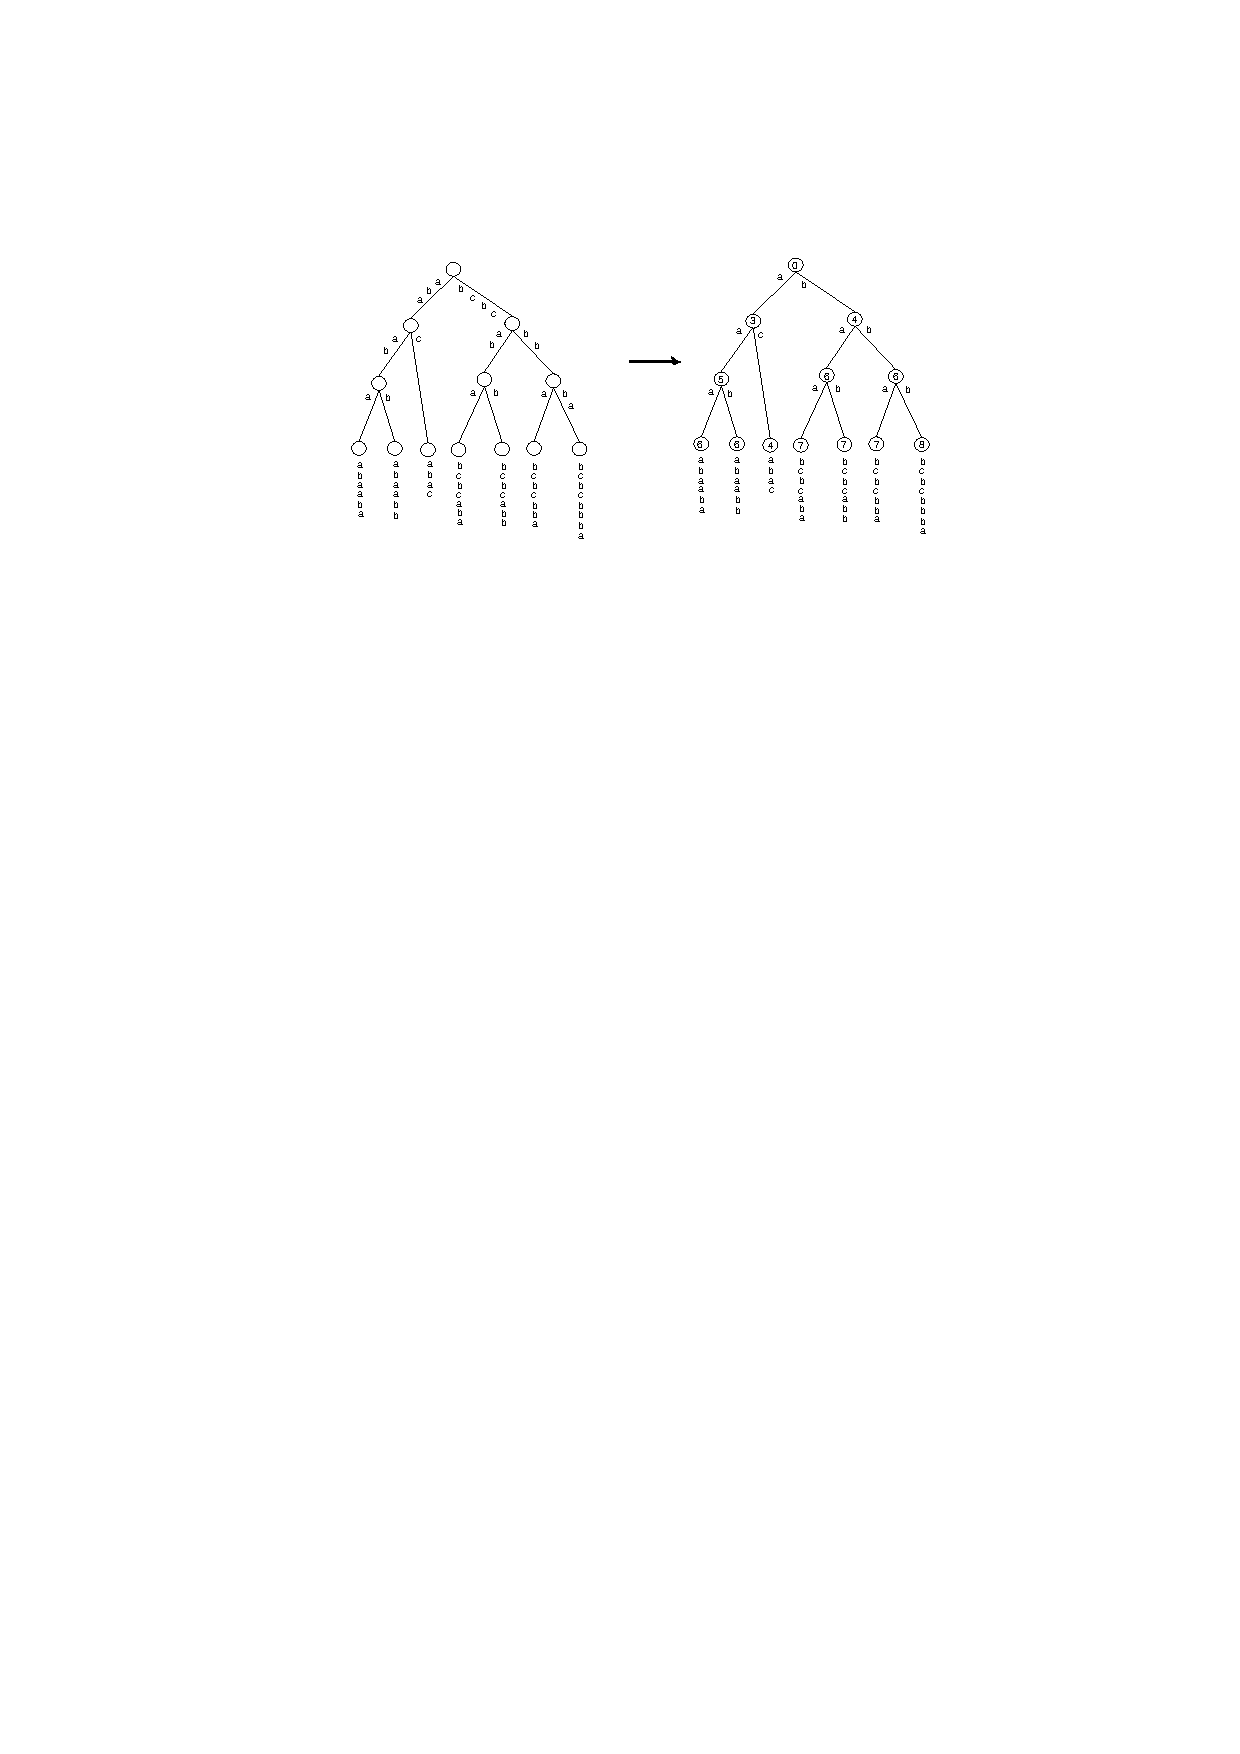
\includegraphics[width=.9\linewidth]{figures/blindtrie.pdf}
    \end{center}
    \caption{Drzewo skompresowane oraz odpowiadające mu drzewo \emph{blind trie}
    zbudowane na zbiorze sekwencji \emph{abaaba, abaabb, abac, bcbcaba, bcbcabb, bcbcbba, bcbcbbba}. 
    Źródło: \cite{MF}.}\label{rys:blind-trie}
\end{figure}

Do sortowania zbiorów większych niż $B$ autorzy algorytmu \emph{deep shallow}
użyli zmodyfikowanego algorytmu \emph{ternary split quicksort}, opisanego w~pracy \cite{bentley-sort}. Dokonali oni następujących zmian:
\begin{enumerate}
  \item Jeżeli na dowolnym etapie rekursji zbiór sufiksów jest mniejszy niż
  $B$, to do jego sortowania użyty zostaje algorytm \emph{blind sort}.
  \item Podczas fazy podziału sufiksów obliczane są $L_S$ i~$L_L$, czyli
  długość najdłuższego wspólnego prefiksu elementu osiowego (\english{pivot}) i~zbioru elementów mniejszych ($L_S$) oraz większych ($L_L$) od elementu
  osiowego. Dzięki temu podczas sortowania sufiksów w~tych zbiorach można
  pomijać prefiksy długości $L_S$ lub $L_L$.
\end{enumerate}

Paolo Ferragina i~Giovanni Manzini w~pracy \cite{MF} wymieniają trzy zalety
dwuetapowego podejścia do problemu sortowania sufiksów zastosowanego w~algorytmie \emph{deep shallow}:
\begin{enumerate}
  \item Szybkie wykrywanie grup sufiksów o~długim wspólnym prefiksie.
  \item Rozmiar stosu użytego podczas rekurencji w~fazie sortowania płytkiego
  jest ograniczony parametrem $L$ i~nie zależy od rozmiaru wejścia.
  \item Jeżeli długość najdłuższego wspólnego prefiksu sufiksów jednego kubełka
  nie przekracza $L$, to uporządkowywane są one efektywnym algorytmem
  sortowania ciągu znaków (\emph{multikey quicksort}).
\end{enumerate}
 
 
\section{Algorytm \emph{two-stage}}

Hideo Itoh i~Hozumi Tanaka zaproponowali w~pracy \cite{IT} algorytm tworzenia
tablic sufiksów o~nazwie \emph{two-stage}. Algorytm ten dzieli sufiksy na dwie
kategorie: sufiksy typu $A$ to wszystkie sufiksy $S_i$ spełniające nierówność $x[i] > x[i+1]$,
sufiksy typu $B$ to sufiksy spełniające nierówność $x[i] \leq x[i+1]$.
 
Algorytm rozpoczyna swoje działanie od obliczenia \SA{1}. Początek i~koniec
każdej grupy zapamiętywany jest w~tablicach $\mathit{head}$ i~$\mathit{tail}$. Długość tych tablic odpowiada wielkości słownika symboli.
Sufiksy w~każdej \emph{1-grupie} są uporządkowywane w~taki sposób, żeby sufiksy typu $A$
były przed sufiksami typu $B$. Wynika to z~tego, że jeżeli sufiksy $S_i$ typu $A$ i~$S_j$ typu $B$ mają wspólny prefiks długości jednego symbolu, to sufiks $S_i$ poprzedza sufiks $S_j$ w~porządku leksykograficznym. Indeksy pierwszych sufiksów typu $B$ każdej
grupy zapamiętywane są w~tablicy $\mathit{part}$ długości $\sigma$.
Kolejnym krokiem algorytmu jest sortowanie sufiksów typu $B$ wewnątrz każdej
grupy. Autorzy pracy \cite{IT} sugerują użycie do tego celu algorytmu
\cite{bentley}, nie jest to jednak konieczne i~można do tego celu użyć innego
algorytmu sortowania ciągów znaków. 


Następnie ustalany jest porządek sufiksów typu $A$. Tablica \SA{} przeglądana
jest od lewej do prawej, znajdując wartości $i=\mathit{SA}[j], j=0,1,\ldots,n-1$. Jeżeli
$S_{i-1}$ jest jeszcze nieuporządkowanym sufiksem typu $A$, to umieszczany jest
na początku grupy do której należy. Odpowiednia wartość w~tablicy \emph{head} jest potem
inkrementowana. Po jednokrotnym przejrzeniu \SA{} sufiksy są już w~pełni
posortowane, co kończy algorytm (przykład na rysunku~\ref{rys:it}).

\begin{figure}[ht]
        \begin{center} \small
            \begin{tabular}{r c c c c c c c c c c c c l}                           
                 & 0  & 1  & 2  & 3  & 4  & 5   & 6  & 7  & 8  & 9  & 10 & 11       \\ \cmidrule{2-13} 
         $x$ = [ & b  & a  & d  & d  & a  & d   & d  & a  & c  & c  & a  &
         $\dollar$ & ] \\ type = [ & A  & B  & B  & A  & B  & B   & A  & B  & B  & A  & A  & B    & ] \\ \addlinespace[1em]
	
       \multicolumn{14}{c}{\emph{1-sort}}\\
       \SA{} = [ & 11 & (-- & 1  & 4  & 7) & (--) & (-- & 8) & (-- & --  & 2  & 5)   & ] \\
        type = [ & B  & A  & B  & B  & B  & A   & A  & B  & A  & A  & B  & B    & ] \\ \addlinespace[1em]
	
       \multicolumn{14}{c}{sortowanie sufiksów typu $B$} \\
       \SA{} = [ & 11 & (-- & 7  & 4  & 1) & (--) & (-- & 8) & (-- & --  & 5  & 2)   & ] \\ \addlinespace[1em]
	
       \multicolumn{14}{c}{wstawianie sufiksów typu $A$}\\
       \SA{} = [ & 11 & 10 & 7  & 4  & 1  & --   & --  & 8  & --  & --  & 5  & 2   & ] \\
       \SA{} = [ & 11 & 10 & 7  & 4  & 1  & --   & 9  & 8  & --  & --  & 5  & 2   & ] \\
       \SA{} = [ & 11 & 10 & 7  & 4  & 1  & --   & 9  & 8  & 6  & --  & 5  & 2   & ] \\
       \SA{} = [ & 11 & 10 & 7  & 4  & 1  & --   & 9  & 8  & 6  & 3  & 5  & 2   & ] \\
       \SA{} = [ & 11 & 10 & 7  & 4  & 1  & 0   & 9  & 8  & 6  & 3  & 5  & 2   & ] \\
            \end{tabular}            
        \end{center}                         
    \caption{Przebieg algorytmu \emph{two-stage} dla słowa ,,baddaddacca''.
    Nieuporządkowane sufiksy typu $A$ oznaczane są znakiem ,,--''. Źródło:
    opracowanie własne na podstawie \cite{taxonomy}.}%
    \label{rys:it}
\end{figure}


\section{Algorytm \emph{improved two-stage}}

Algorytm \emph{improved two-stage} opisany został w~pracy \cite{MP}, której
autorami są Simon Puglisi i~Michael Maniscalco.
Kwestia autorstwa tego algorytmu pozostaje niejasna, metoda ta posiada aż trzy niezależne
implementacje powstałe przed publikacją artykułu:
\begin{itemize}
	\item \emph{archon } [\ref{archon}] autorstwa Dimy Małyszewa,
	\item \emph{divsufsort} [\ref{libdivsufsort}] której autorem jest Yuta Mori,
	\item \emph{msufsort} [\ref{msufsort}] autorstwa Michaela Maniscalco.
\end{itemize}
Wymienione implementacje algorytmu \emph{improved two-stage} napisane zostały w~języku \texttt{C++}. 

Na początku sufiksy są dzielone na dwie kategorie: sufiksy typu $A$ to sufiksy
$S_i$ spełniające nierówność $S_i > S_{i+1}$, sufiksy typu $B$ to sufiksy
spełniające nierówność $S_i \leq S_{i+1}$. Sufiks o~identyfikatorze $n-1$ należy
do obu grup. Następnie, sufiksy $S_i$ typu $B$ których następny sufiks $S_{i+1}$ jest typu $A$ oznaczane są jako
sufiksy typu $B^*$. 

Kolejnym krokiem algorytmu jest znalezienie granic grup które powstałyby po
\emph{2-sortowaniu}. Następnie tworzony jest \emph{2-porządek} sufiksów typu
$B^*$. \emph{2-sortowanie} wszystkich sufiksów nie jest konieczne w~tym
momencie, a~jego pominięcie zmniejsza czas działania algorytmu.
Sufiksy typu $B^*$ należące do jednej grupy są sortowane zgodnie z~metodami
przedstawionymi w~pracach \cite{bentley, MF} i~umieszczane na początkowych
pozycjach wewnątrz kubełka w~tablicy \SA{}. 

Porządek sufiksów typu $B$ ustalany jest poprzez przeglądanie tablicy \SA{} od
prawej do lewej. Dla każdego sufiksu $\mathit{SA}[i]$ odczytanego podczas
przeglądania tablicy sufiks $\mathit{SA}[i]-1$ jest wstawiany na ostatnią pustą
pozycję wewnątrz swojej grupy jeżeli jest sufiksem typu $B$.

Wstawianie sufiksów typu $A$ wykonywane jest w~sposób identyczny jak w~algorytmie
\emph{two-stage} (przykład przedstawiono na rysunku \ref{rys:div}).

\begin{figure}[t]
        \begin{center}\small  
            \begin{tabular}{r c c c c c c c c c c c c c c l}                           
                 & 0   & 1  & 2   & 3      & 4  & 5 & 6  & 7      & 8   & 9  & 10 & 11    & 12  & 13      \\\cmidrule{2-15} 
         $x$ = [ & e   & d  & a   & b      & d  & c & c  & d      & e   & e  &
         d  & a     & b   & $\dollar$ & ] \\ type = [ & A   & A  & B   & $B^*$  & A  & B & B  & $B^*$  & A   & A  & A  & $B^*$ & A   &      &  ] \\ \addlinespace[1em]
	\multicolumn{16}{c}{Obliczanie wielkości \emph{2-grup}}\\
      \SA{2} = [ & --  & (-- & --) & --     & --  & -- & --  & (--     & --) & --  & -- & (--    & --)  & --    & ] \\ \addlinespace[1em]
    \multicolumn{16}{c}{Sortowanie sufiksów typu $B^*$} \\
       \SA{} = [ & --   & 11 & --   & --      & 3  & -- & --  & --      & --   & --  & 7  & --     & --   & --    & ] \\ \addlinespace[1em]  
	\multicolumn{16}{c}{Wstawianie sufiksów typu B}\\
       \SA{} = [ & --   & 11 & --   & --      & 3  & -- & 6  & --      & --   & --  & 7  & --     & --   & --    & ] \\  
       \SA{} = [ & --   & 11 & --   & --      & 3  & 5 & 6  & --      & --   & --  & 7  & --     & --   & --    & ] \\  
       \SA{} = [ & --   & 11 & 2   & --      & 3  & 5 & 6  & --      & --   & --  & 7  & --     & --   & --    & ] \\ \addlinespace[1em]
	\multicolumn{16}{c}{Wstawianie sufiksów typu A}\\
       \SA{} = [ & 13  & 11 & 2   & --      & 3  & 5 & 6  & --      & --   & --  & 7  & --     & --   & --    & ] \\  
       \SA{} = [ & 13  & 11 & 2   & 12     & 3  & 5 & 6  & --      & --   & --  & 7  & --     & --   & --    & ] \\  
       \SA{} = [ & 13  & 11 & 2   & 12     & 3  & 5 & 6  & 10     & --   & --  & 7  & --     & --   & --    & ] \\  
       \SA{} = [ & 13  & 11 & 2   & 12     & 3  & 5 & 6  & 10     & 1   & --  & 7  & --     & --   & --    & ] \\  
       \SA{} = [ & 13  & 11 & 2   & 12     & 3  & 5 & 6  & 10     & 1   & 4  & 7  & --     & --   & --    & ] \\  
       \SA{} = [ & 13  & 11 & 2   & 12     & 3  & 5 & 6  & 10     & 1   & 4  & 7  & 9     & --   & --    & ] \\  
       \SA{} = [ & 13  & 11 & 2   & 12     & 3  & 5 & 6  & 10     & 1   & 4  & 7  & 9     & 0   & --    & ] \\  
       \SA{} = [ & 13  & 11 & 2   & 12     & 3  & 5 & 6  & 10     & 1   & 4  & 7  & 9     & 0   & 8    & ] \\  
            \end{tabular}            
        \end{center}                         
    \caption{Przebieg algorytmu \emph{divsufsort} dla słowa ,,edabdccdeedab''.
 			Źródło: opracowanie własne na podstawie \cite{div}.}%
    \label{rys:div}
\end{figure}


\section{Algorytm \emph{bpr}}

Klaus-Bernd Schürmann w~pracy \cite{schurmann-phd} zaproponował algorytm
\emph{bpr} (\emph{bucket pointer refinement}, polepszanie wskaźników na
kubełki). Algorytm ten jest poprawioną wersją metody przedstawionej w~pracy
\cite{bpr-old} napisanej przez Klausa-Bernda Schürmanna i~Jensa Stoye. Kod
algorytmu \emph{bpr} w~języku \texttt{C++} dostępny jest na stronie [\ref{bpr-code}].

Pierwszym krokiem algorytmu jest posortowanie sufiksów według $q$-pierwszych
znaków, czyli \emph{q-sortowanie}. Wartość parametru $q$ obliczana jest na
podstawie liczby różnych symboli (czyli wielkości alfabetu) w~ciągu wejściowym, jej wartość maleje wraz ze
wzrostem wielkości słownika sekwencji wejściowej. Następnie obliczana jest
przybliżona odwrotna tablica sufiksów \ISA{} (kubełki identyfikowane są pozycją
ich ostatniego elementu w~przybliżonej tablicy sufiksów), nazywana w~pracy
\cite{schurmann-phd} \emph{tablicą wskaźników na kubełki}.

Algorytm \emph{bpr} działa według schematu \emph{polepszania kubełków wgłąb} i~korzysta z~techniki \emph{pull}. Sufiksy $S_i$ i~$S_j$ należące
do jednej \emph{h-grupy} porównywane są poprzez porównanie wartości
\ISA{}$[h + i]$ i~\ISA{}$[h + j]$.

Każda ze znalezionych na początku grup sortowana jest algorytmem \emph{ternary
split quicksort} \cite{bentley-sort}. Parametr $h$ przyjmuje początkowo
wartość $q$. Algorytm ten wybiera jeden z~sufiksów danej grupy jako element
osiowy (\english{pivot}) $S_p$ o~wartości klucza $K_p = \textit{ISA}[h + p]$. Sufiksy danej grupy dzielone są na trzy
podgrupy: sufiksy o~wartości klucza mniejszej, równej lub większej niż $K_p$.
Każda z~tych podgrup jest następnie w~ten sam sposób sortowana, przy czym
dla grupy sufiksów o~wartości klucza równej elementowi osiowemu wartość
parametru $h$ zwiększana jest o~$q$, ponieważ wszystkie jej sufiksy mają
wspólny prefiks długości $h + q$. Wynika to z~tego, że elementy kubełka o~wspólnym prefiksie długości $h$ sortowane są na podstawie pozycji ich
\emph{h-następników}, dla których nie znamy długości wspólnego prefiksu.
Wiadomo tylko tyle, że były posortowane na początku działania algorytmu według
$q$ pierwszych znaków. Podobnie jak w~algorytmie \emph{qsufsort}, równa wartość
klucza $\textit{ISA}[h + i]$ i~$\textit{ISA}[h + j]$ oznacza że sufiksy $S_i$ i~$S_j$ mają wspólny prefiks długości $h+q$. Fundamentalna różnica między
algorytmami \emph{bpr} i~\emph{qsufsort} polega na tym, że pierwszy z~nich
realizuje schemat \emph{polepszania kubełków wgłąb}, a~drugi \emph{polepszania
wszerz}. Dzięki temu, algorytm \emph{qsufsort} w~kolejnej iteracji może
podwajać wartość parametru $h$.

Istotną cechą algorytmu \emph{bpr} jest to, że po każdym podziale grupy na
podgrupy wykonywana jest aktualizacja wpisów w~tablicy \ISA{} odpowiadających
jej elementom, zgodnie ze wzorem $\textit{ISA}[i] =$ \emph{pozycja
ostatniego elementu podgrupy}. Na rysunku \ref{rys:bpr} przedstawiony został
przebieg działania algorytmu \emph{bpr} na przykładzie ciągu ,,DEBDEBDEA''.

\begin{figure}[t]
    \begin{center}\small
    \begin{tabular}{r c c c c c c c c c l}
                     &  0   &      1      &      2      &      3      &     4      &      5      &     6      &      7      &      8      &     \\ \cmidrule{2-10} 
               $x=[$ &  D   &      E      &      B      &      D      &     E      &      B      &     D      &      E      &      A      & ]   \\ \addlinespace[.5em] 
                                                  \multicolumn{11}{c}{Podział na kubełki, $q=2$}                                                \\ 
                     &  A   &  \multicolumn{2}{c}{BD}   &         \multicolumn{3}{c}{DE}         &     EA     &  \multicolumn{2}{c}{EB}   &     \\ 
     $\textit{SA}=[$ &  8   & \textbf{(2} & \textbf{5)} &     (0      &     3      &     6)      &     7      &     (1      &     4)      & $]$ \\ 
    $\textit{ISA}=[$ &  5   &      8      &      2      &      5      & \textbf{8} &      2      &     5      & \textbf{6}  &      0      & $]$ \\ \addlinespace[.5em] 
                                                  \multicolumn{11}{c}{Po posortowaniu kubełka BD}                                               \\ 
     $\textit{SA}=[$ &  8   &      5      &      2      & \textbf{(0} & \textbf{3} & \textbf{6)} &     7      &     (1      &     4)      & $]$ \\ 
    $\textit{ISA}=[$ &  5   &      8      & \textbf{2}  &      5      &     8      & \textbf{1}  &     5      &      6      & \textbf{0}  & $]$ \\ \addlinespace[.5em] 
                                                  \multicolumn{11}{c}{Po posortowaniu kubełka DE}                                               \\ 
     $\textit{SA}=[$ &  8   &      5      &      2      &      6      &     3      &      0      &     7      & \textbf{(1} & \textbf{4)} & $]$ \\ 
    $\textit{ISA}=[$ &  5   &      8      &      2      & \textbf{4}  &     8      &      1      & \textbf{3} &      6      &      0      & $]$ \\ \addlinespace[.5em] 
                                         \multicolumn{11}{c}{Po posortowaniu kubełka EB, koniec algorytmu}                                      \\ 
     $\textit{SA}=[$ &  8   &      5      &      2      &      6      &     3      &      0      &     7      &      4      &      1      & $]$ \\ 
    $\textit{ISA}=[$ &  5   &      8      &      2      &      4      &     7      &      1      &     3      &      6      &      0      & $]$ \\ 
    \end{tabular}
    \end{center}

    \caption{Przebieg algorytmu \emph{bpr} dla słowa ,,DEBDEBDEA''. Elementy
    wyróżnione w~tablicy \emph{SA} przeznaczone do uporządkowania w~danym
    kroku, elementy wyróżnione w~tablicy \ISA{} to klucze wykorzystywane 
   do sortowania kubełka. Źródło: opracowanie własne na podstawie
   \cite{schurmann-phd}.}\label{rys:bpr}
\end{figure}


\chapter{Testy wydajnościowe}

\section{Wstęp}
 
W~poniższym rozdziale przedstawione zostaną wyniki testów wydajnościowych implementacji algorytmów
opisanych w~poprzedniej części pracy (poza algorytmem \emph{two-stage}, który został rozwinięty
i~poprawiony przez \emph{improved two-stage}). Implementacja w~języku \texttt{Java} została oparta
o~oryginalny kod, udostępniony przez autorów. Podstawą implementacji metody \emph{improved
two-stage} był kod algorytmu \emph{divsufsort} napisany przez Yutę Moriego [\ref{libdivsufsort}].

Algorytmy tworzenia tablic sufiksów zaimplementowane zostały w~ten sposób, żeby na wejściu
przyjmowały sekwencje liczb całkowitych typu \texttt{int} zajmujących w~języku \texttt{Java} 4
bajty. Spowodowało to zwiększenie złożoności pamięciowej algorytmów (wartości podane w~tabeli
\ref{tab:alg} zakładały wejście w~postaci sekwencji jednobajtowych elementów). Powodem zwiększenia
rozmiaru pojedynczego elementu wejściowego było umożliwienie tworzenia tablic sufiksów dla sekwencji
symboli z~alfabetów o~dużym rozmiarze. Nie jest to jednak możliwe w~praktyce w~przypadku wszystkich
algorytmów; rzeczywista złożoność pamięciowa implementacji wybranych metod oraz ich zależność od
rozmiaru alfabetu wejściowego opisane zostały w~tabeli \ref{tab:alg-impl}. Testowane implementacje
algorytmów \emph{bpr}, \emph{deep-shallow} i~\emph{qsufsort} dla zaoszczędzenia pamięci nadpisywały
ciąg wejściowy. Na potrzeby testów wydajnościowych zaimplementowano również naiwny algorytm
tworzenia tablic sufiksów opierający się o~zwykły algorytm sortujący \emph{quicksort}. W~dalszej
części rozdziału metoda naiwna nazywana będzie \emph{naive sort} lub NS.

Wykonane testy algorytmów można podzielić na dwie główne kategorie: testy na wejściu generowanym
losowo, oraz testy na wejściu wczytywanym z~plików. Testy drugiego typu wykonywane były na kilku
różnych maszynach wirtualnych:

\begin{itemize}
    \item maszyna Java HotSpot 64-Bit Server VM 11.0-b16 firmy Sun Microsystems, oznaczana w~dalszej części pracy jako \texttt{sun},
    \item maszyna IBM J9 VM 2.4 firmy IBM, oznaczana w~dalszej części pracy jako \texttt{ibm},
    \item BEA JRockit(R) R27.5.0-110\_o-99226-1.6.0\_03 firmy BEA (aktualnie przejęta przez Oracle), oznaczana w~dalszej części pracy jako \texttt{jrockit},
    \item Apache Harmony DRLVM 11.2.0 tworzona przez Apache Software Foundation, oznaczana w~dalszej części pracy jako \texttt{harmony}.
\end{itemize} 

\begin{table}[ht]
    \begin{center}        
        \begin{tabular}{l r r}
         \toprule
            Nazwa & Złożoność pamięciowa \\
         \midrule
            \emph{skew} & $16n$  \\
            \emph{bpr} & $4|\Sigma|^3+12n$ \\ 
            \emph{deep-shallow} & $4|\Sigma|^2+(x+8)n$  \\
            \emph{divsufsort} & $4|\Sigma|^2+8n$ \\
            \emph{qsufsort} & $8n$ \\
            \emph{naive sort} & $8n$ \\
        \bottomrule
        \end{tabular}
    \end{center}                         
    \caption{Zaimplementowane algorytmy tworzenia tablic sufiksów. Parametr $n$ oznacza długość wejścia, 
    parametr $|\Sigma|$ oznacza wielkość alfabetu sekwencji wejściowej. Algorytm \emph{deep-shallow} wymaga
    alfabetu o~rozmiarze nie większym niż 256, zużycie pamięci przez ten 
    algorytm zależy od wielkości budowanego drzewa \emph{blind trie}, które maksymalnie może zawierać $n$ elementów. Rozmiar jednego elementu drzewa wynosi $x=48$ bajtów na 64-bitowej maszynie wirtualnej firmy Sun.
    Algorytmy \emph{bpr} i~\emph{divsufsort} nie mają sztywnych ograniczeń na rozmiar 
    alfabetu, ale ze względu na wydajność nie powinny być używane na dużych alfabetach.}%
    \label{tab:alg-impl}
\end{table}
	
\noindent
Testy przeprowadzone zostały na kilku komputerach testowych o~następujących parametrach:
\begin{itemize}
    \item dwurdzeniowy procesor Athlon 5200 o~prędkości 2.6 GHz, 64-bitowy system operacyjny OpenSuSE, jądro w~wersji 2.6.22.19-0.2-default,
    \item czterordzeniowy procesor Intel Xeon x3230 o~prędkości 2.66 GHz, 64-bitowy system operacyjny OpenSuSE, wersja jądra 2.6.22.19-0.2-default,
    \item jednordzeniowy Intel Pentium 4 o~prędkości 3 GHz, 32-bitowy system operacyjny Windows XP.
\end{itemize}
	
\noindent
Wszystkie obliczenia przeprowadzone zostały z~parametrami maszyn wirtualnych
odpowiadającym opcjom ,,\texttt{-Xmx2g -server}'' -- zwiększają one maksymalny rozmiar 
sterty do 2Gb, a~maszyna wirtualna pracuje w~trybie ,,serwerowym'' (agresywna optymalizacja JIT).
	
Czas działania algorytmów mierzony był przez klasę uruchamiającą testy, poprzez liczenie różnicy
wartości zwracanych przez metodę \texttt{System.currentTimeMillis()} przed i~po obliczeniach
(tzw.~\emph{wall time}). Do mierzenia zużycia pamięci wykorzystano specjalnie w~tym celu napisany
aspekt [\ref{aspectj}]. Mierzone było zużycie pamięci wewnątrz wirtualnej maszyny na początku
działania algorytmu, pod jego koniec oraz po zakończeniu wybranych metod wewnątrz klas. Mierzenie
zużycia pamięci w~języku \texttt{Java} jest trudne, bowiem maszyna wirtualna nie pozwala na dokładne
oszacowanie wszystkich dokonanych alokacji pamięci. Do celów testowych posłużono się programowaniem
aspektowym i~,,wpleciono'' (\english{code weaving}) dynamiczne instrukcje mierzące różnicę
w~aktualnej ilości zaalokowanej pamięci względem startu algorytmu. Nie jest to oszacowanie idealne,
ale pozwala na zgrubne stwierdzenie ile pamięci zużywa dany algorytm.

Test na jednej instancji wejścia (pliku lub wygenerowanej sekwencji o~ustalonych parametrach)
powtarzany był 10 razy, a~jego wynikiem jest średnia z~zebranych pomiarów. Testy których wyniki
zbierano poprzedzano kilkoma uruchomieniami algorytmu. Celem tego zabiegu było wyeliminowanie błędów
pomiarowych wynikających z~wolniejszego działania kodu, który nie został skompilowany do kodu
natywnego przez maszynę wirtualną. Testy na wejściu generowanym losowo były poprzedzone 10 rundami
,,rozgrzewki", natomiast przed testem na wejściu wczytywanym z~pliku algorytm uruchamiany był 5
razy.
	
W~dalszej części rozdziału prezentowane są wyniki pochodzące z~pomiarów na komputerze z~procesorem
Xeon x3230. Wyniki z~pozostałych maszyn są niemal identyczne pod względem porównywania i~rankingu
algorytmów, dlatego też w wielu miejscach je pominięto (wszystkie wyniki są na dołączonej do pracy
płycie CD). Samo porównanie efektywności wykonania programów w różnych maszynach wirtualnych
znajduje się w rozdziale \ref{sect:vms}.


\section{Testy wydajnościowe na losowo generowanym wejściu}

Celem testów na losowo generowanym wejściu jest zbadanie rzeczywistej zależności algorytmów od
długości wejścia, wielkości alfabetu oraz średniego \emph{lcp} ciągu wejściowego. Testy
przeprowadzono tylko na jednej maszynie wirtualnej (\texttt{sun}). Ziarno generatora liczb losowych
otrzymywało identyczną wartość przed testem każdego algorytmu by zapewnić powtarzalność wyników.
	
	
\subsection{Wejście o~zmiennej długości i~stałej wielkości alfabetu}

Testy algorytmów na losowym wejściu o~zmiennej długości i~stałej wielkości alfabetu powtórzono trzy
razy. Każdy test wykonany był dla wejścia generowanego z~alfabetu wielkości 4,100 i~255 elementów.
Rysunek \ref{rys:random-input-lcp} przedstawia średnią wartość \emph{lcp} generowanych ciągów
wejściowych. Z~rysunku wynika, że wartość średniego \emph{lcp} jest mniej więcej odwrotnie
proporcjonalna do wielkości alfabetu.
		
Rysunki \ref{rys:random-input-time-4} i~\ref{rys:random-input-memory-4} przedstawiają czas działania
algorytmów oraz zużycie pamięci dla alfabetu wielkości 4. Algorytmy \emph{qsufsort} i~\emph{naive
sort} uzyskały najlepszy wynik złożoności pamięciowej. Zgodnie z~przewidywaniami, algorytmy
\emph{skew} i~\emph{deep shallow} wypadł najgorzej w~tej kwestii. Najszybszym algorytmem okazał się
być algorytm \emph{bpr}. Wyraźnie wolniejsze od pozostałych algorytmów są algorytmy \emph{skew}
i~\emph{naive sort}.


\begin{figure}[t]
       \begin{center}
            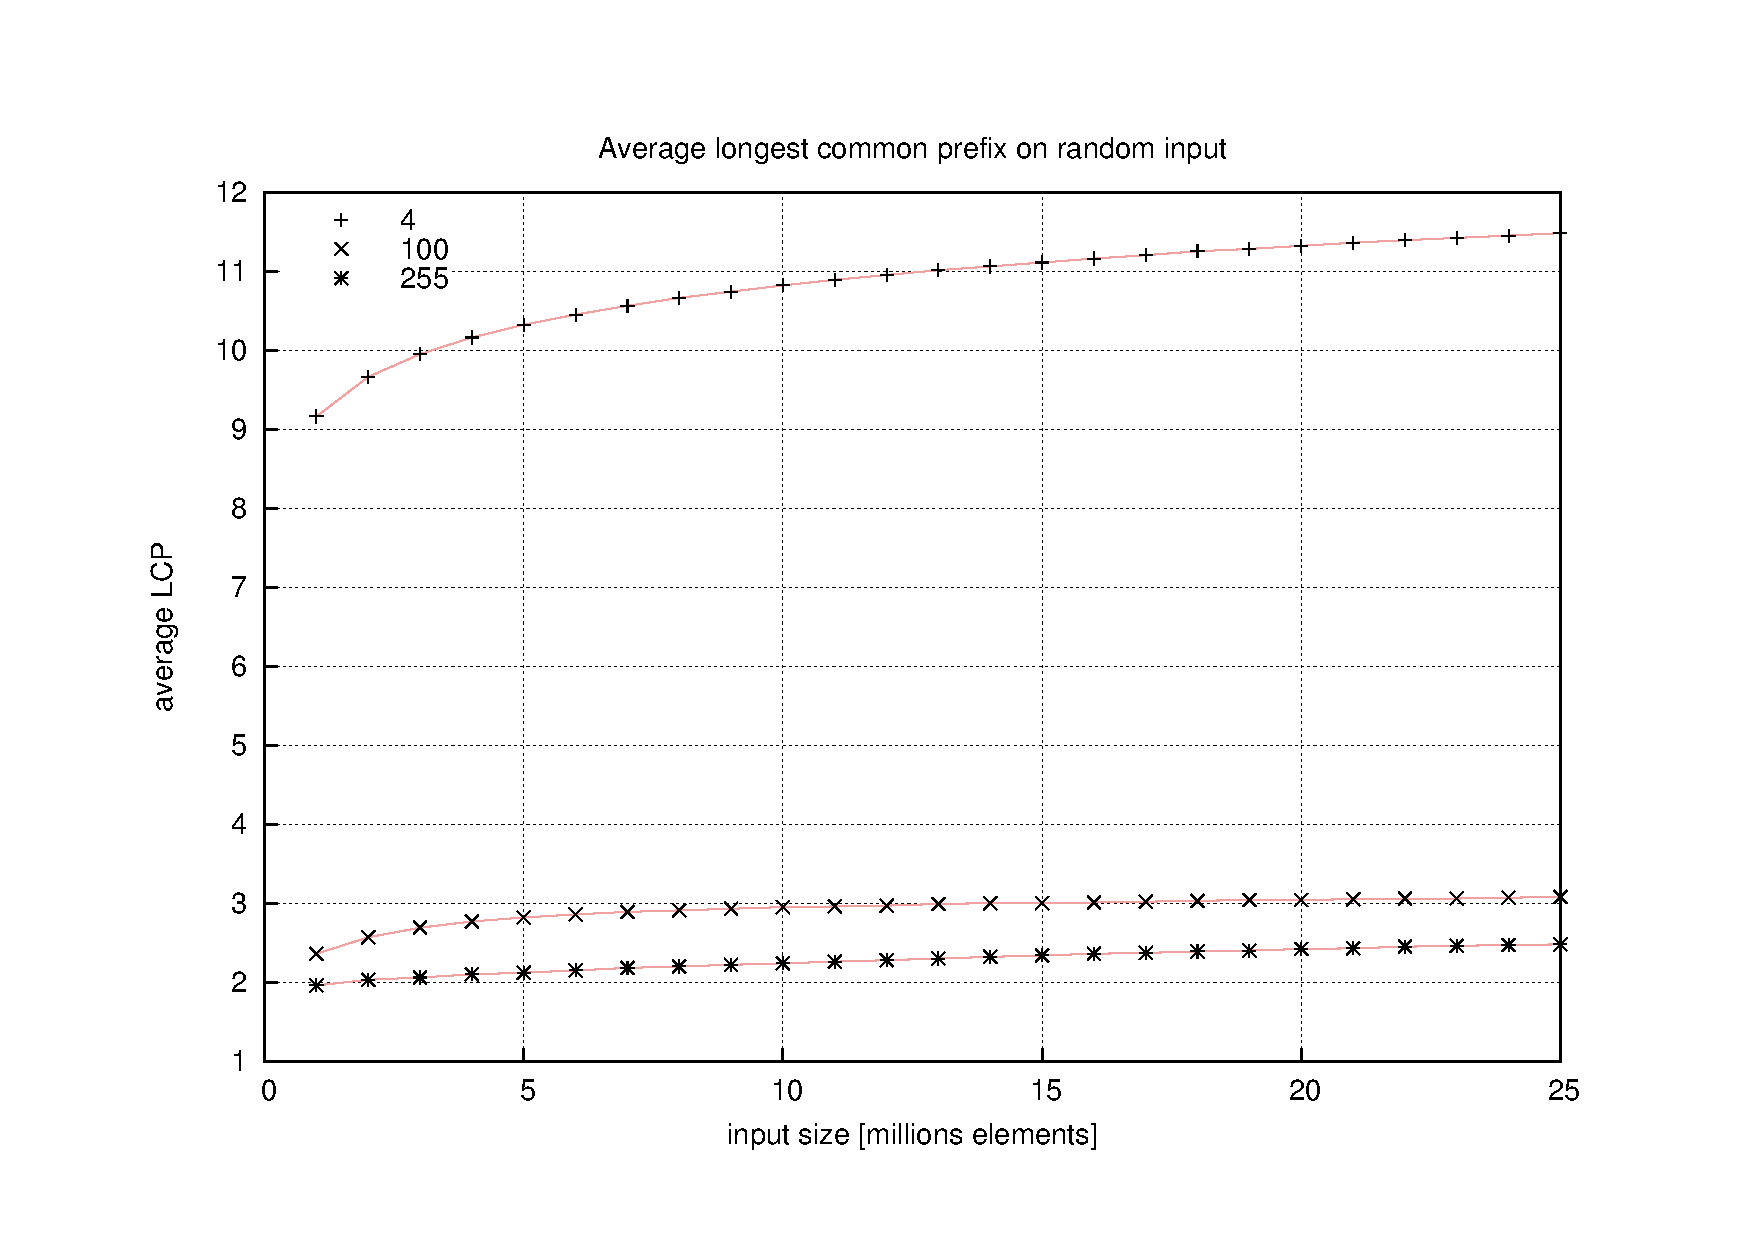
\includegraphics[width=\linewidth]{figures/results/random-input-lcp}
        \end{center}
    \caption{Średnie \emph{lcp} w~zależności od długości wejścia dla alfabetów o wielkości 4, 100 i~255 symboli.}%
    \label{rys:random-input-lcp}
\end{figure}

\begin{figure}[tp]
    \begin{center}
          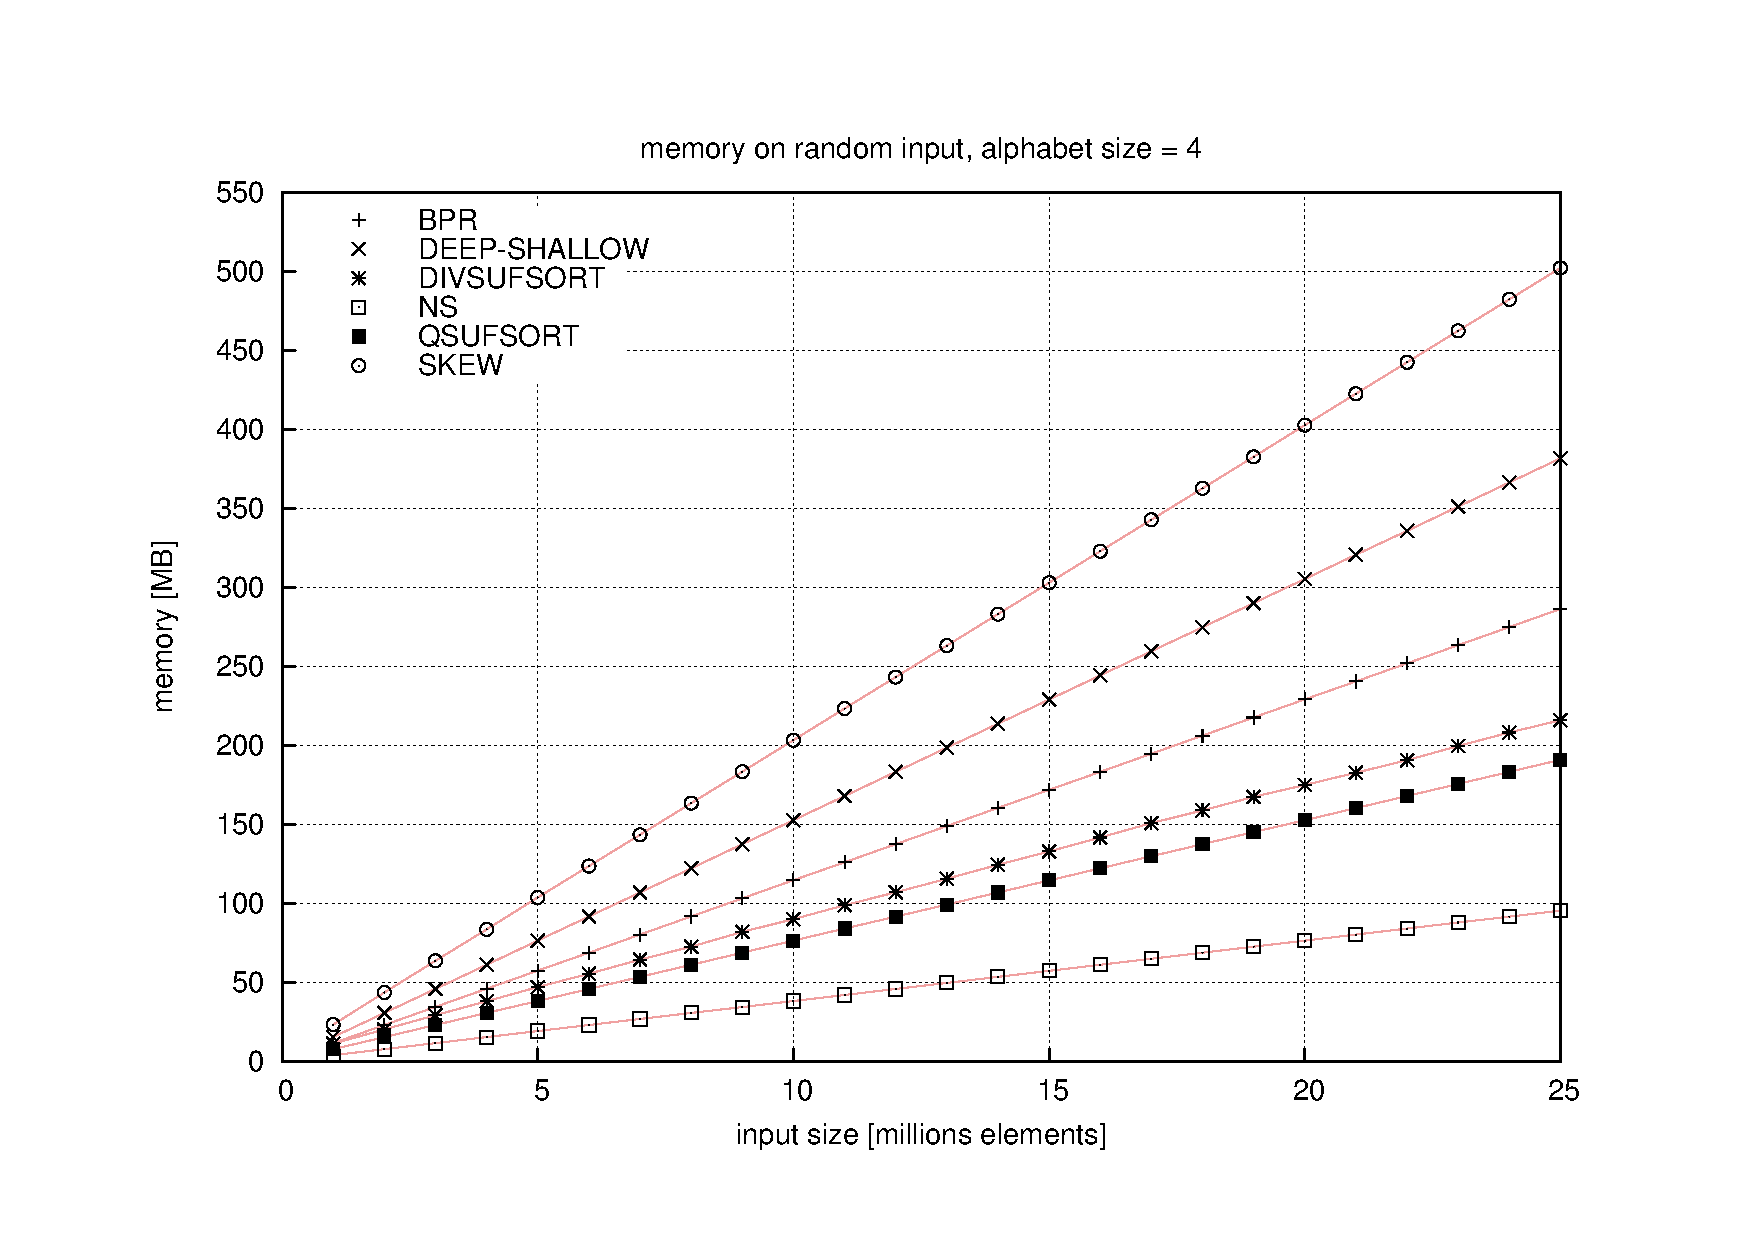
\includegraphics[width=\linewidth]{figures/results/random-input-memory-4}
    \end{center}
    \caption{Zużycie pamięci w~zależności od długości wejścia generowanego z~alfabetu wielkości 4.}%
    \label{rys:random-input-memory-4}
\end{figure}

%TODO wyniki zuzycia pamieci przez naive sort wskazuja na zaniżone wyniki pomiarów -- powinny być podobne wartości jak dla algorytmu qsufsort.
\begin{figure}[tp]
       \begin{center}
            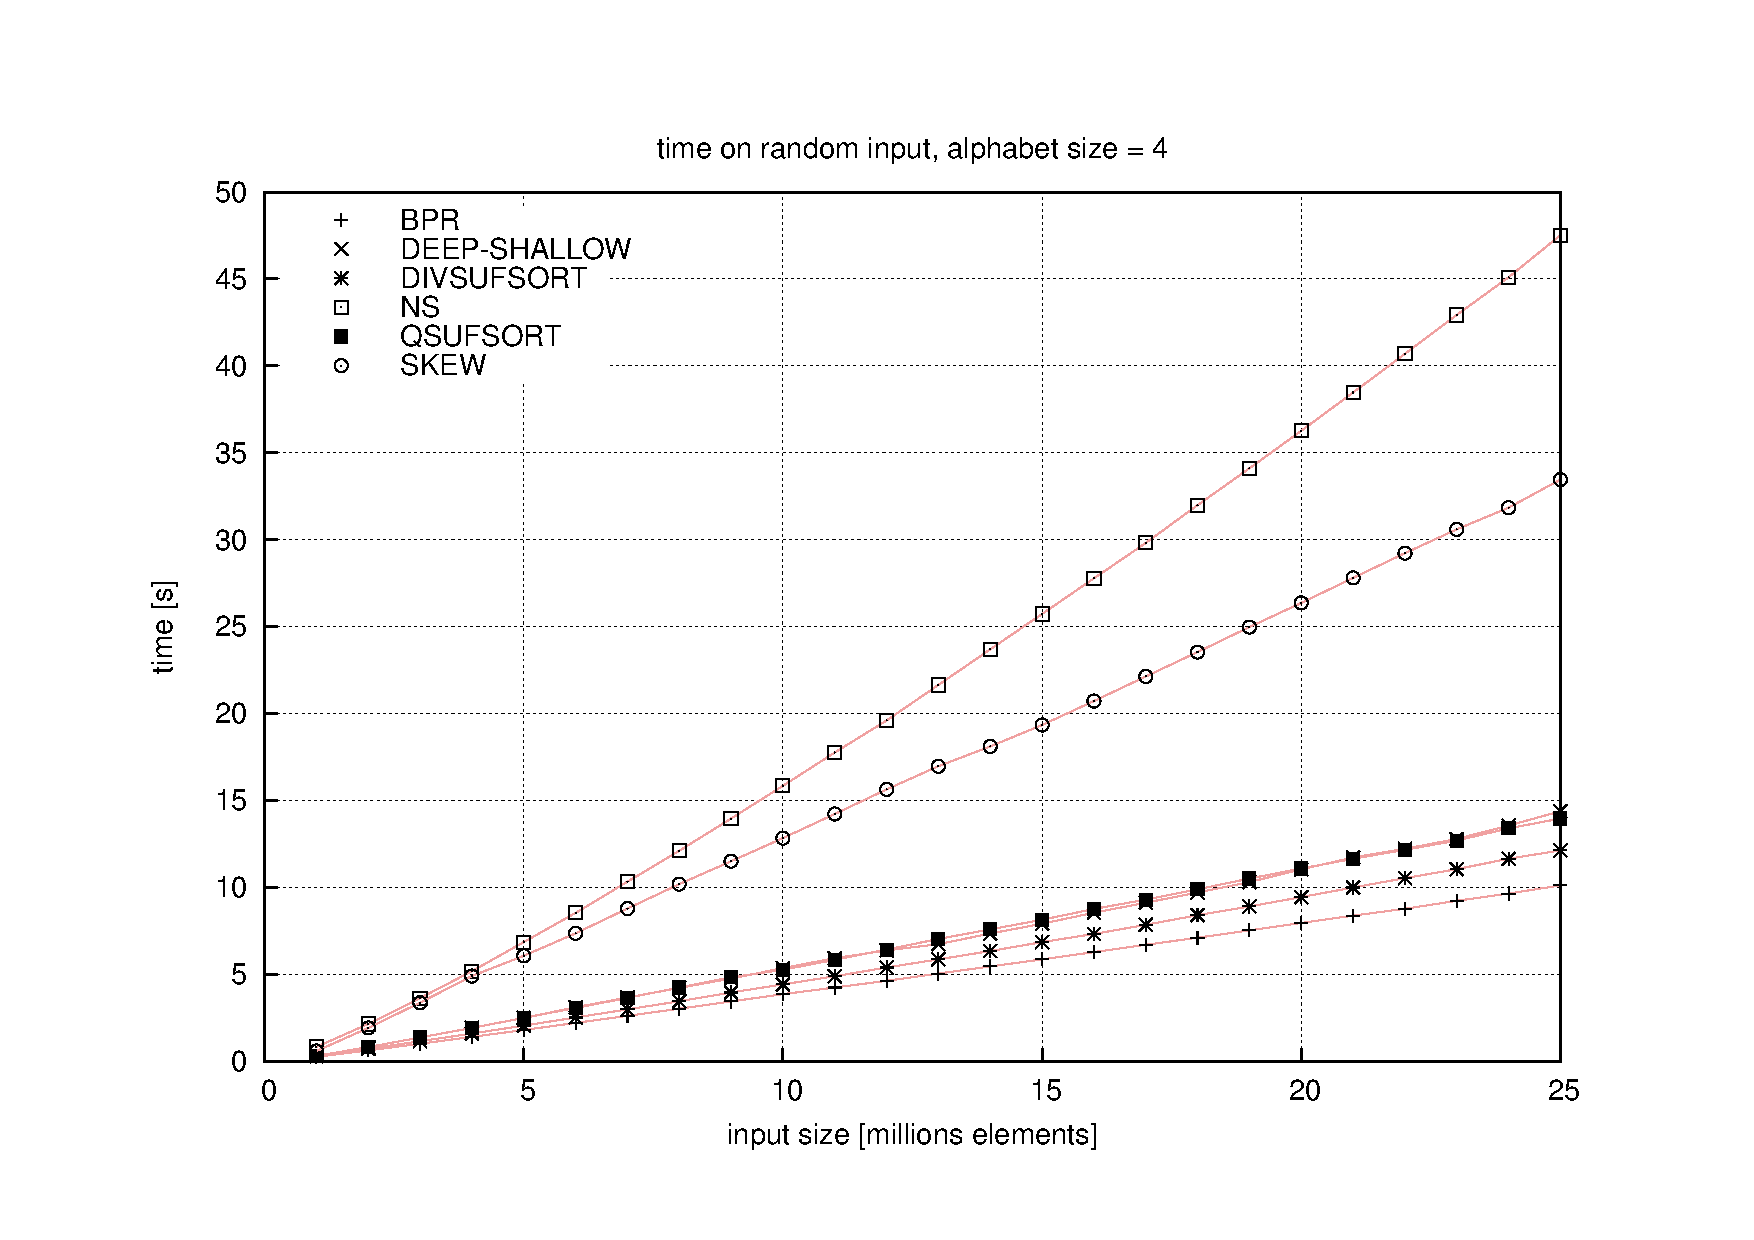
\includegraphics[width=\linewidth]{figures/results/random-input-time-4.pdf}
        \end{center}        
    \caption{Czas działania algorytmów w~zależności od długości wejścia generowanego z~alfabetu wielkości 4.}%
    \label{rys:random-input-time-4}
\end{figure}

\begin{figure}[tp]
   \begin{center}
      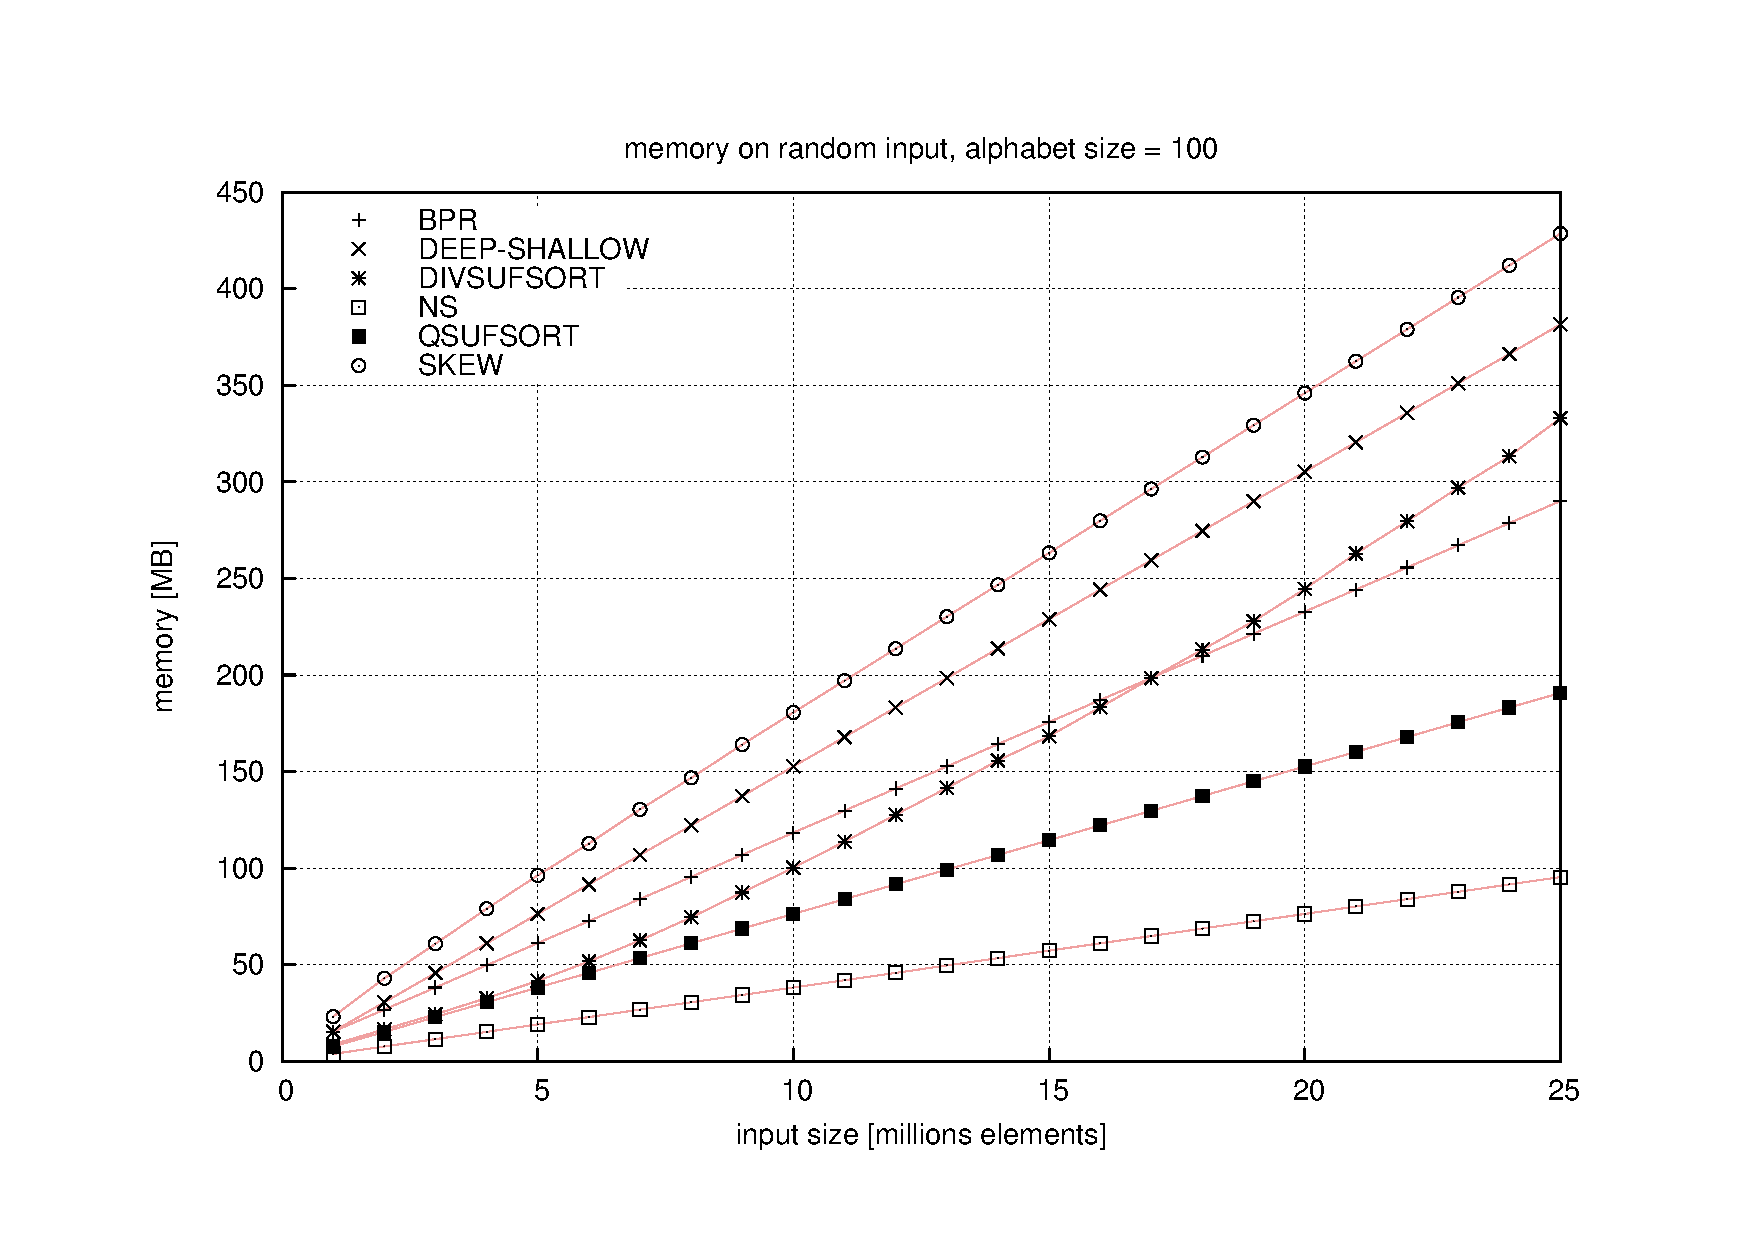
\includegraphics[width=\linewidth]{figures/results/random-input-memory-100.pdf}
    \end{center}        
    \caption{Zużycie pamięci w~zależności od długości wejścia generowanego z~alfabetu wielkości 100.}%
    \label{rys:random-input-memory-100}
\end{figure}

% nie wiem jak wyjaśnić zwiekszone zuzycie pamieci przez algorytm divsufsort
Wyniki testów wejścia generowanego z~alfabetu wielkości 100 przedstawione są na rysunku
\ref{rys:random-input-time-100} i~\ref{rys:random-input-memory-100}.
Rezultaty testu czasu działania algorytmu są niemal identyczne jak poprzedniego. Jedyną różnicą jest
to, że algorytm \emph{bpr} nie uzyskał najlepszego wyniku lecz znalazł się wśród kilku algorytmów
uzyskujących bardo dobry wynik, zajął również więcej pamięci.

\begin{figure}[tp]
   \begin{center}
        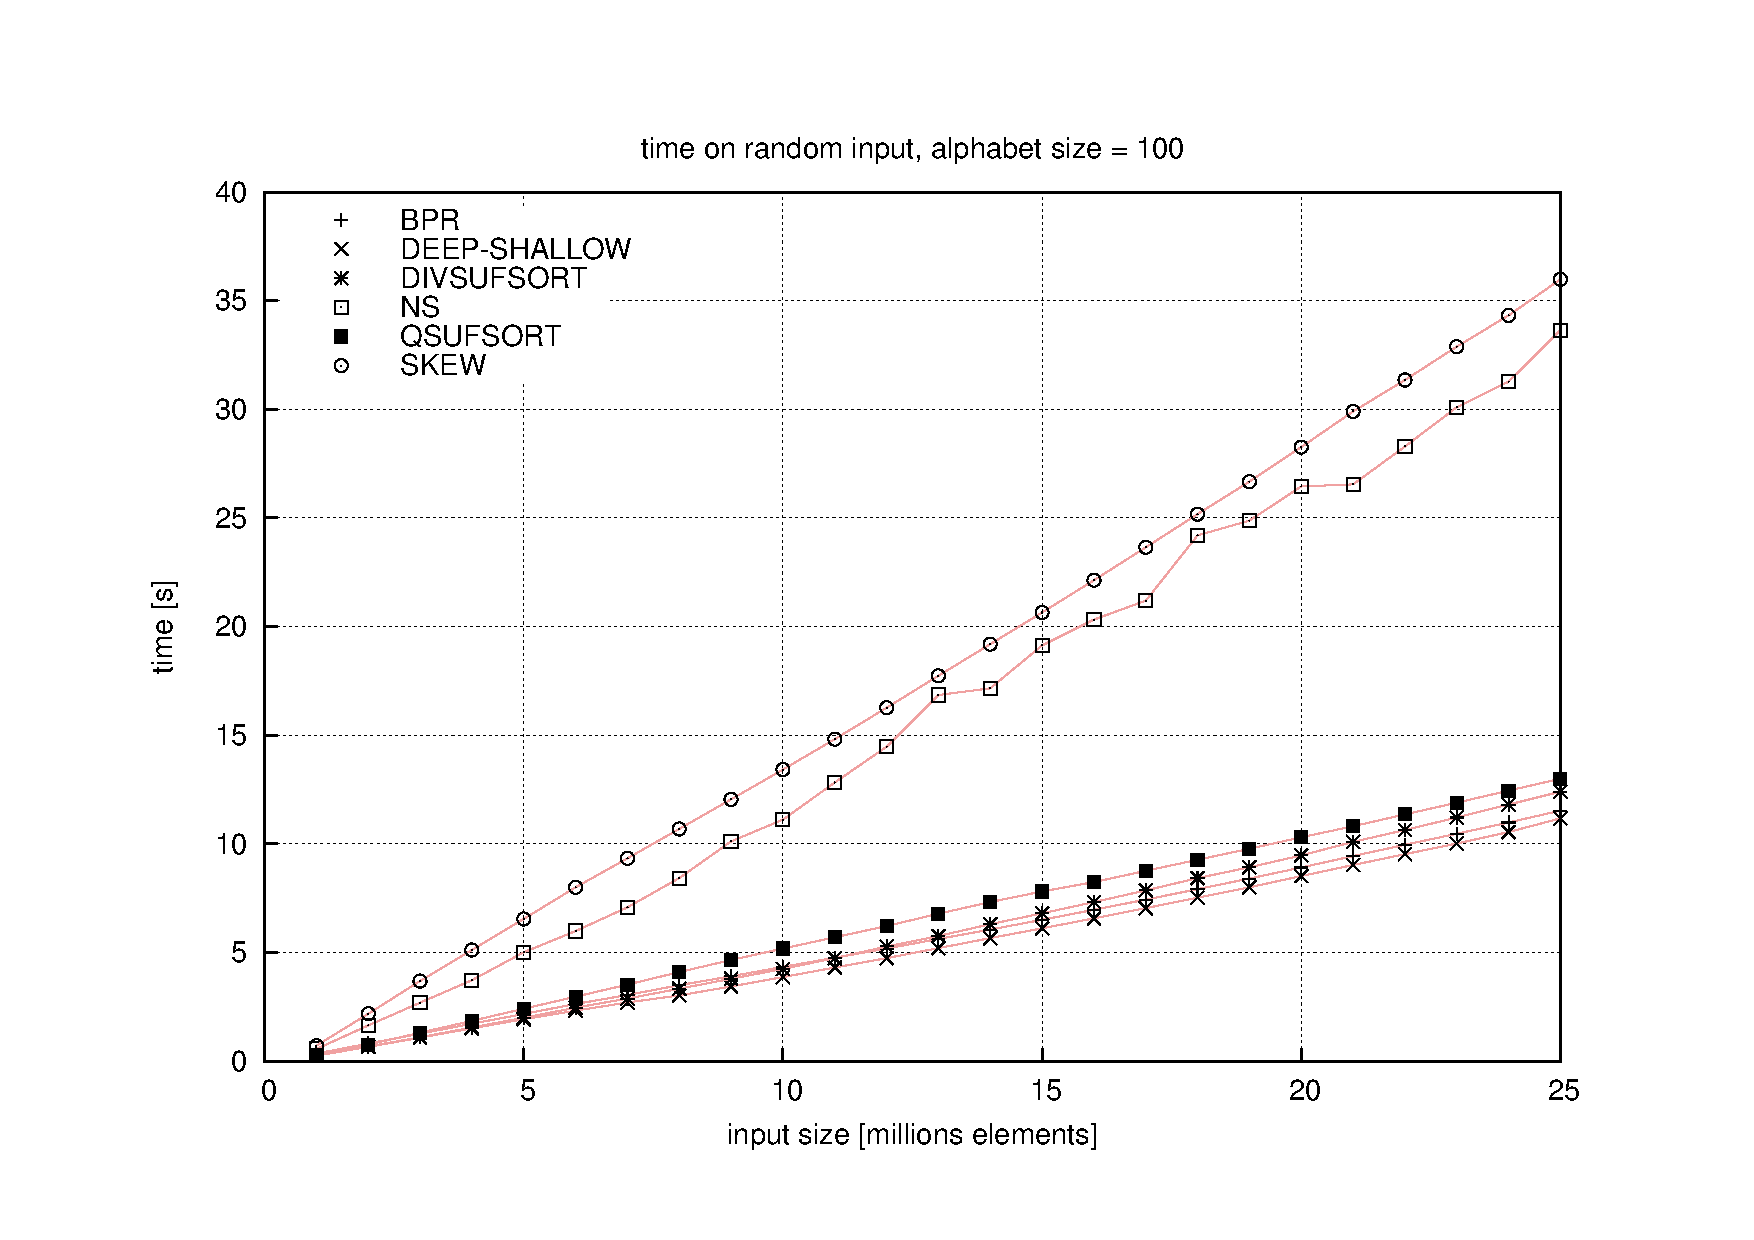
\includegraphics[width=\linewidth]{figures/results/random-input-time-100.pdf}
    \end{center}        
    \caption{Czas działania algorytmów w~zależności od długości wejścia generowanego z~alfabetu wielkości 100.}%
    \label{rys:random-input-time-100}
\end{figure} 

Rysunki \ref{rys:random-input-time-255} i~\ref{rys:random-input-memory-255} prezentują wyniki testów
wejścia generowanego z~alfabetu wielkości 255. Wynik tego testu są również podobne do poprzedników.
Algorytm \emph{bpr} uzyskał jeszcze gorszy wynik niż w~poprzednich testach, zajął więcej pamięci
i~działał wolniej od większości algorytmów.

\begin{figure}[tp]
       \begin{center}
          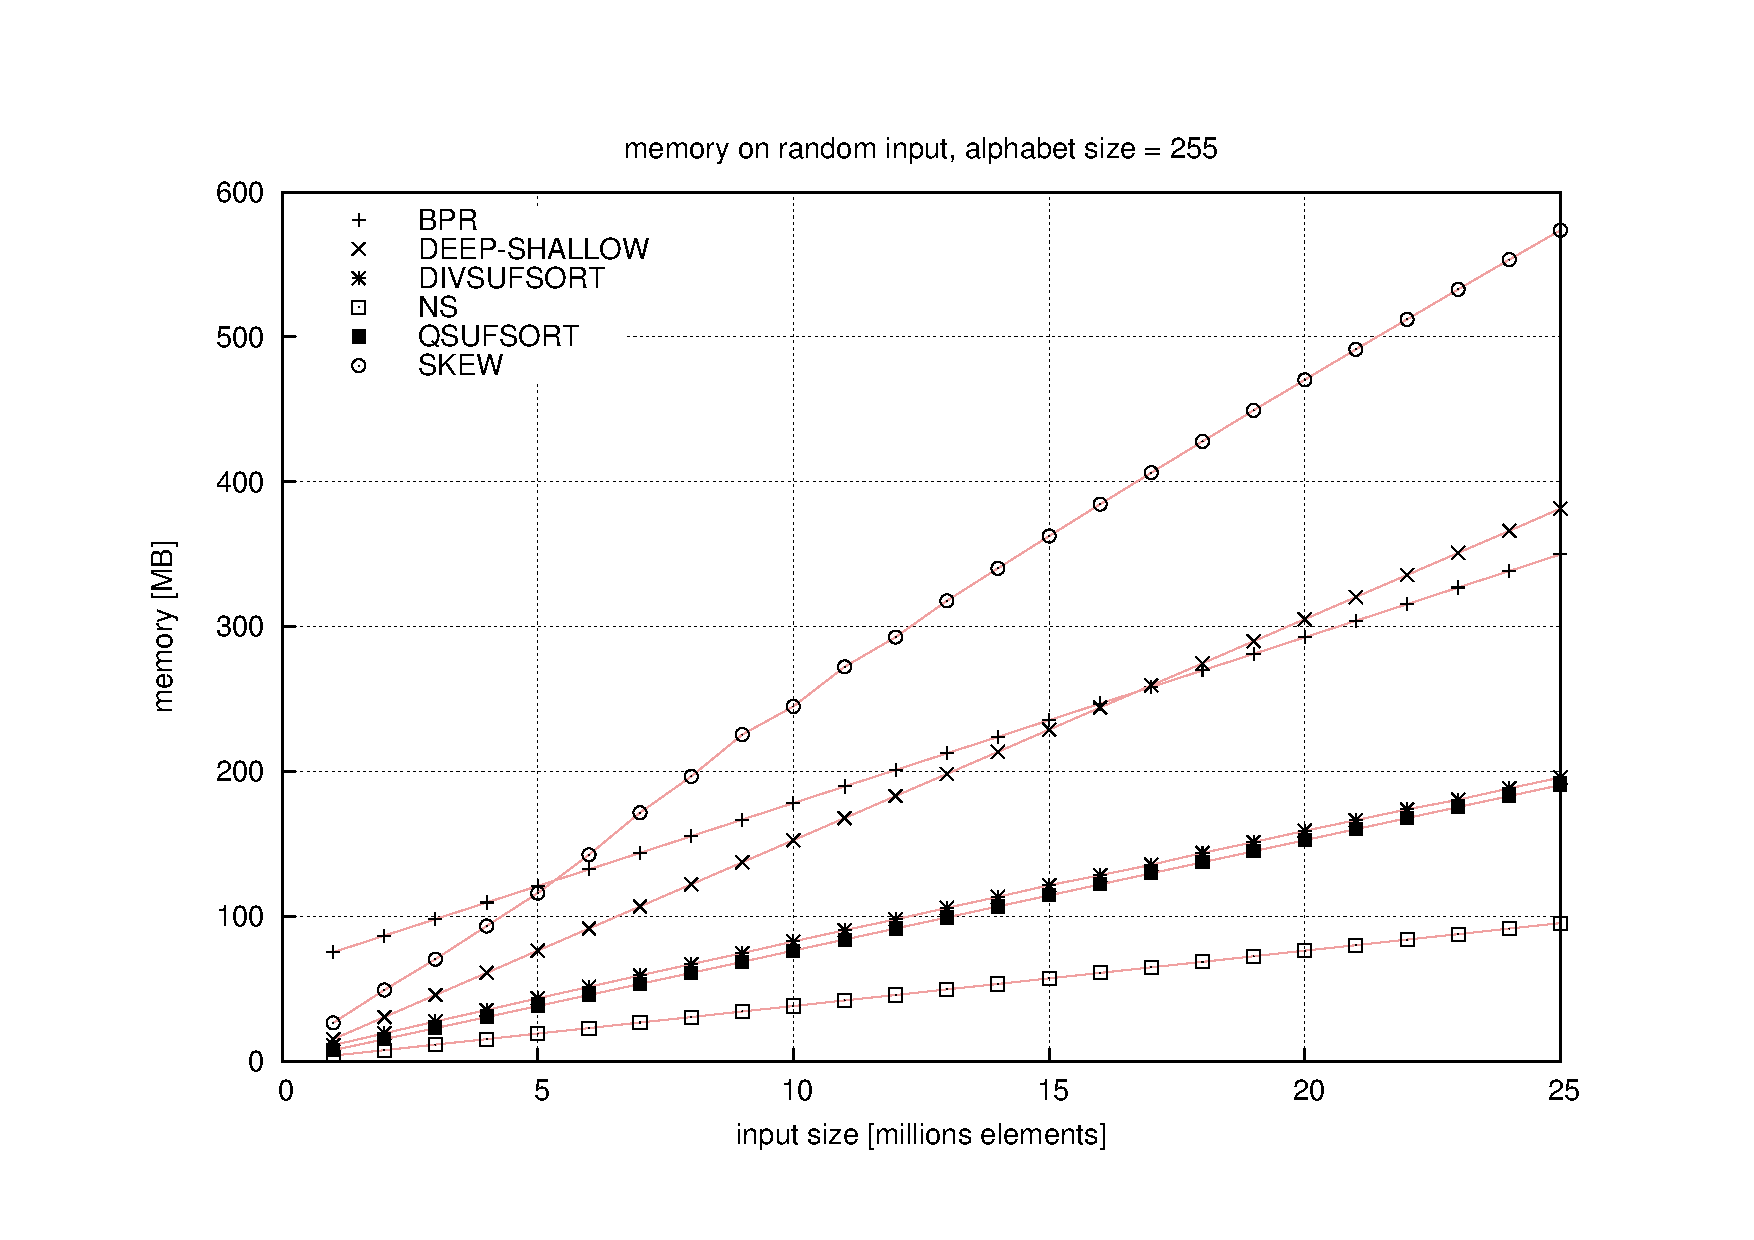
\includegraphics[width=\linewidth]{figures/results/random-input-memory-255.pdf}
        \end{center}        
    \caption{Zużycie pamięci w~zależności od długości wejścia generowanego z~alfabetu wielkości 255.}%
    \label{rys:random-input-memory-255}
\end{figure}

\begin{figure}[tp]
       \begin{center}
            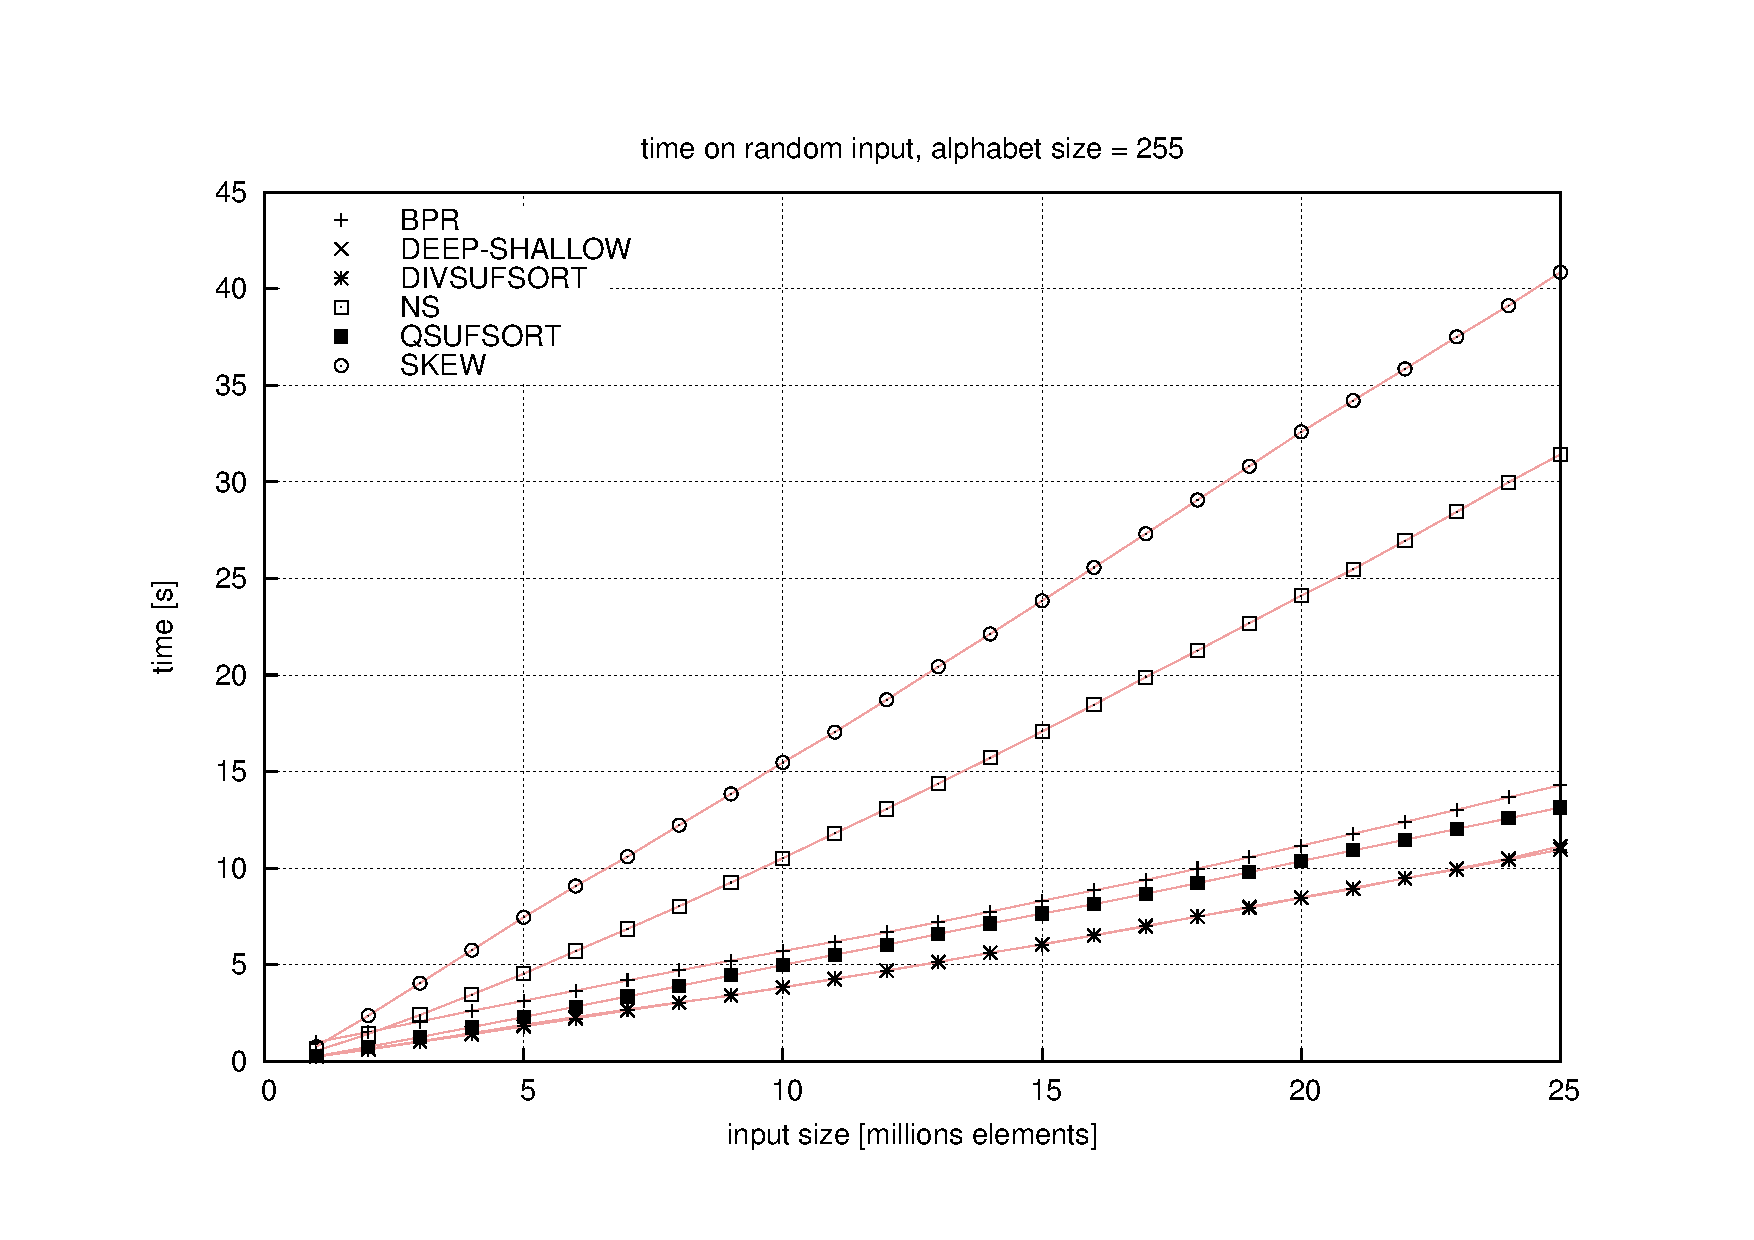
\includegraphics[width=\linewidth]{figures/results/random-input-time-255.pdf}
        \end{center}        
    \caption{Czas działania algorytmów w~zależności od długości wejścia generowanego z~alfabetu wielkości 255.}%
    \label{rys:random-input-time-255}
\end{figure} 


\subsection{Wejście o~stałej długości i~zmiennej wielkości alfabetu}

Wejście generowane na potrzeby testu miało długość 5\,000\,000 elementów. Wykres
\ref{rys:random-alphabet-lcp} przedstawia średnie \emph{lcp} wygenerowanego wejścia w~zależności od
wielkości alfabetu. Wykres \ref{rys:random-alphabet-time} przedstawia czasy działania algorytmów na
generowanym wejściu.

Wyniki testu pokazują które algorytmy zależą od średniego \emph{lcp} i~wielkości alfabetu sekwencji
wejściowej. Algorytm \emph{bpr} jest tego najlepszym przykładem -- im większa jest jedna z~tych
wartości, tym gorzej sobie radzi. Algorytm \emph{skew} uzyskuje lepsze wyniki dla sekwencji
o~większej wartości średniego \emph{lcp}. Pozostałe algorytmy nie wykazują większej zależności
pomiędzy czasem ich działania a~wielkością alfabetu i~średnim \emph{lcp}.
		
\begin{figure}[p]
       \begin{center}
            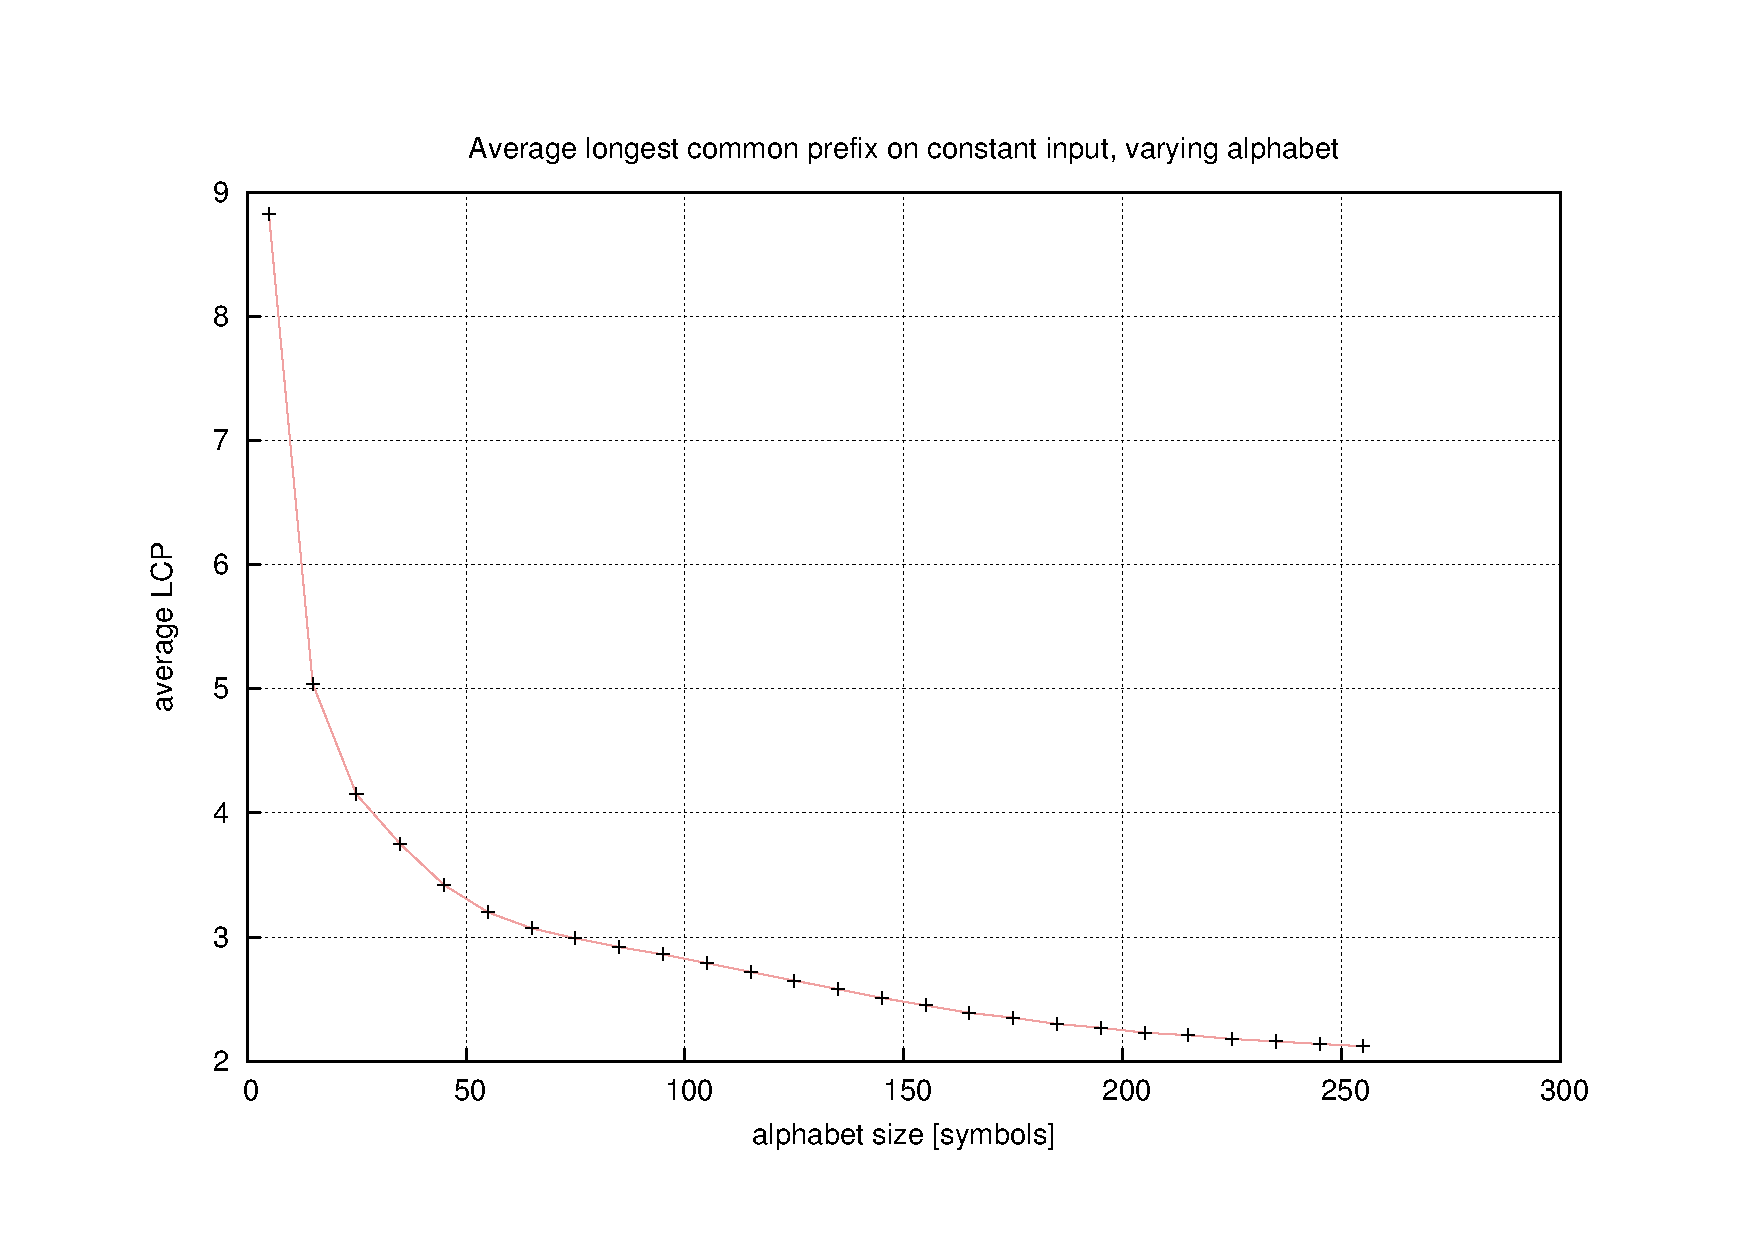
\includegraphics[width=\linewidth]{figures/results/random-alphabet-lcp.pdf}
        \end{center}        
    \caption{Średnie \emph{lcp} generowanego wejścia w~zależności od wielkości alfabetu.}%
    \label{rys:random-alphabet-lcp}
\end{figure}

\begin{figure}[p]
       \begin{center}
            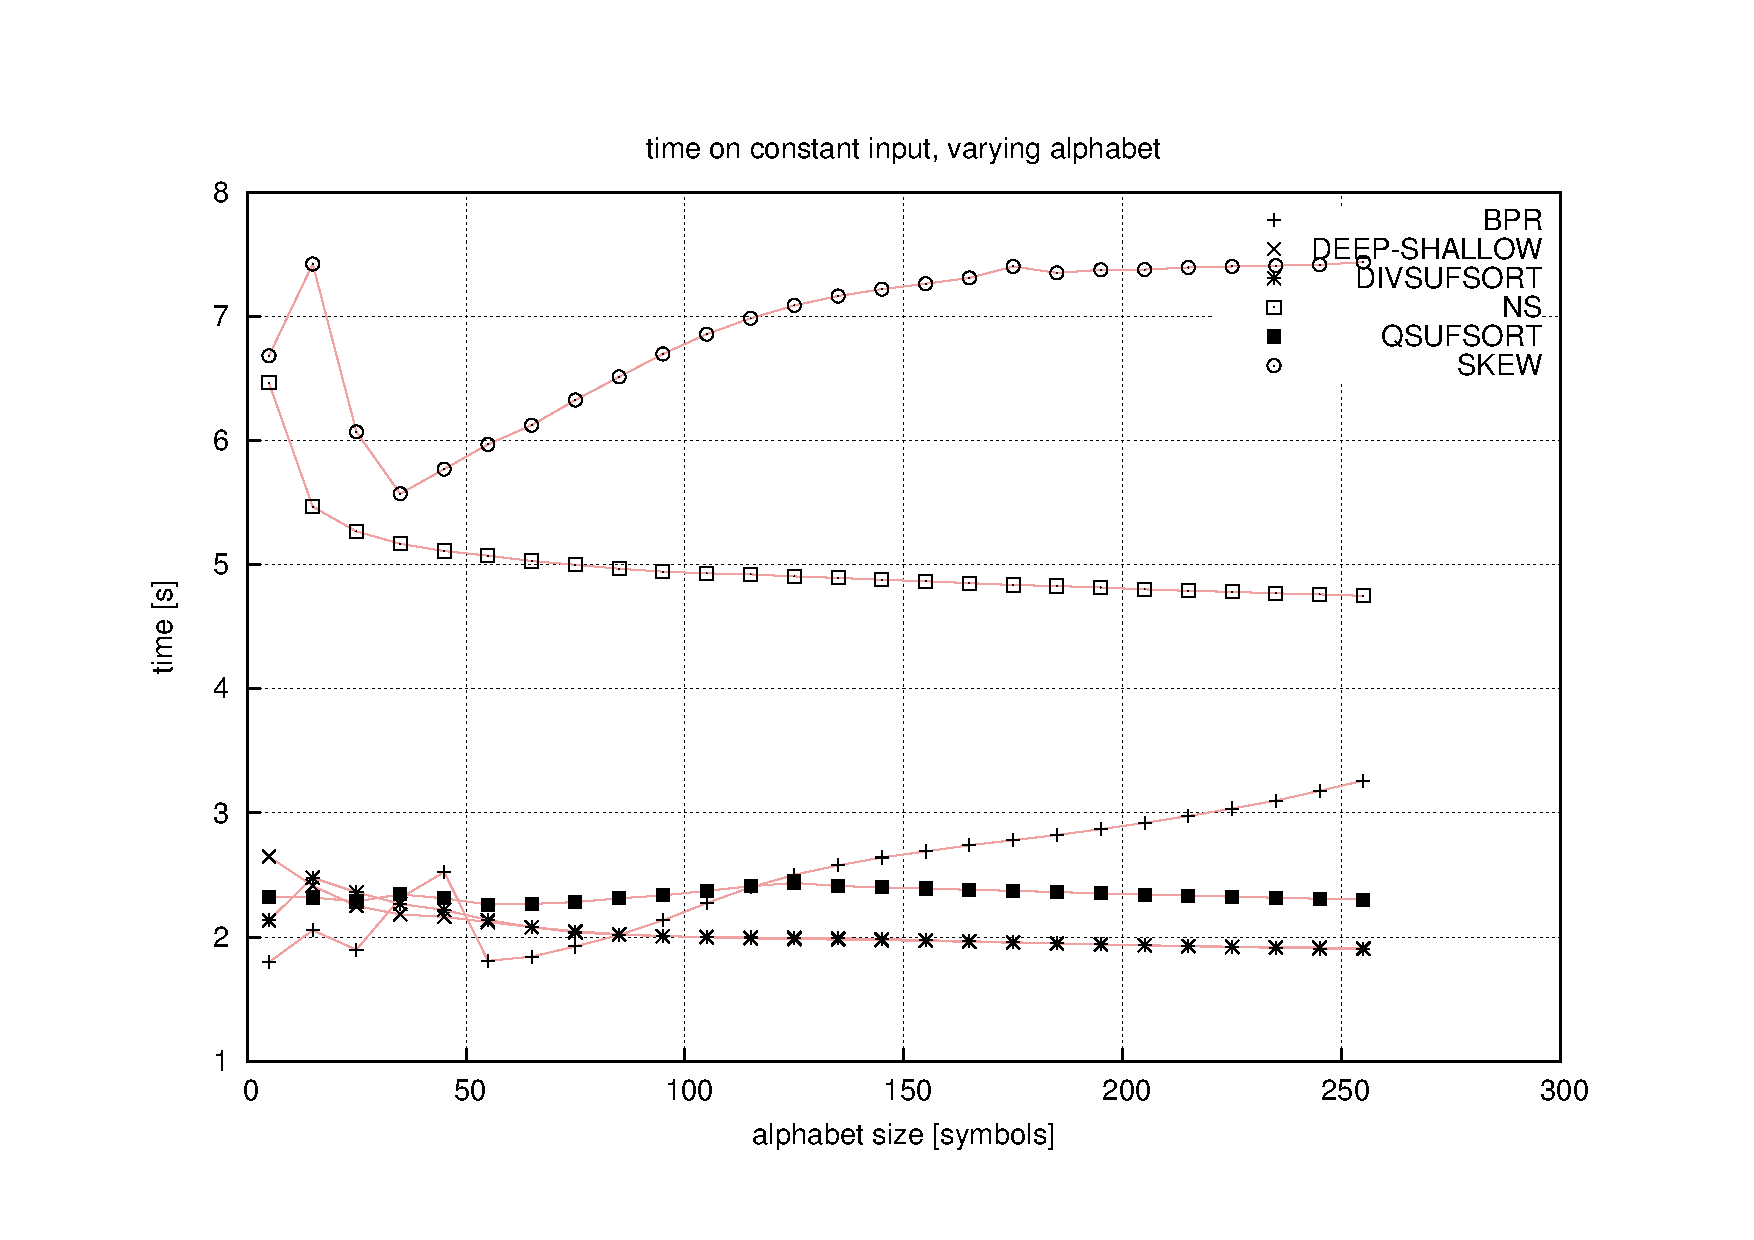
\includegraphics[width=\linewidth]{figures/results/random-alphabet-time.pdf}
        \end{center}        
    \caption{Czas działania algorytmów w~zależności od wielkości alfabetu.}%
    \label{rys:random-alphabet-time}
\end{figure}


% Flush manually before the main section.
\FloatBarrier

\section{Testy wydajnościowe na wejściu wczytywanym z~plików}

Zaimplementowane algorytmy przetestowane zostały na dwóch zestawach plików (korpusach) specjalnie
przygotowanych do testowania algorytmów tworzenia tablic sufiksów. Pierwszy z~nich nosi nazwę
\texttt{Gauntlet}, powstał z~inicjatywy Michaela Maniscalco. Ideą stojącą za stworzeniem tego
korpusu było zebranie plików o~nietypowej strukturze w~celu testowania algorytmów na szczególnych
przypadkach wejścia. Wkład w~powstanie tego zbioru plików wnieśli Yuta Mori, Simon Puglisi oraz
Graham Houston. Korpus dostępny jest do pobrania pod adresem [\ref{gauntlet}].

Drugi korpus testowy opracowany został przez Giovanniego Manziniego. W~jego skład wchodzą
rzeczywiste pliki o~dużym rozmiarze pochodzące z~różnych źródeł. Zestaw plików dostępny jest do
pobrania pod adresem [\ref{manzini-corpus}]. Tabela \ref{tab:manzini-files} prezentuje
charakterystykę plików obu korpusów.

\begin{table}[ht]
    \begin{center} \small
    \begin{tabular}{l r r}
    \toprule
    Plik                    & Rozmiar           & Średnie \emph{lcp} \\ \midrule
    \texttt{abac}           &          200\,000 &         99\,997 \\         
    \texttt{abba}           &      10\,500\,600 &     2\,773\,939 \\         
    \texttt{book1x20}       &      15\,375\,420 &     6\,938\,159 \\         
    \texttt{fib\_s14930352} &      14\,930\,352 &     3\,940\,597 \\         
    \texttt{fss10}          &      12\,078\,908 &     2\,454\,179 \\         
    \texttt{fss9}           &       2\,851\,443 &        579\,353 \\         
    \texttt{houston}        &       3\,840\,000 &         52\,083 \\         
    \texttt{paper5x80}      &          981\,924 &        239\,421 \\         
    \texttt{test1}          &       2\,097\,152 &     1\,048\,064 \\         
    \texttt{test2}          &       2\,097\,152 &     1\,048\,064 \\         
    \texttt{test3}          &       2\,097\,152 &        984\,064 \\         
    \bottomrule
    \end{tabular}
    \hspace{1cm}
    \begin{tabular}{l r r}
    \toprule
    Plik                     & Rozmiar           & Średnie \emph{lcp} \\ \midrule
    \texttt{chr22.dna}       &      34\,553\,758 &          1\,979 \\         
    \texttt{etext99}         &     105\,277\,340 &          1\,108 \\         
    \texttt{gcc-3.0.tar}     &      86\,630\,400 &          8\,603 \\         
    \texttt{howto}           &      39\,422\,105 &             267 \\         
    \texttt{jdk13c}          &      69\,728\,899 &             678 \\         
    \texttt{linux-2.4.5.tar} &     116\,254\,720 &             479 \\         
    \texttt{rctail96}        &     114\,711\,151 &             282 \\         
    \texttt{rfc}             &     116\,421\,901 &              93 \\         
    \texttt{sprot34.dat}     &     109\,617\,186 &              89 \\         
    \texttt{w3c2}            &     104\,201\,579 &         42\,299 \\
    \bottomrule
    \\
    \end{tabular}
    
    \end{center}                         
    \caption{Charakterystyka plików wchodzących w~skład korpusu \texttt{Gauntlet}
    (po lewej) i~korpusu Giovanniego Manziniego (po prawej). Rozmiar i~średnie \emph{lcp} podano w bajtach.}%
    \label{tab:gauntlet-files}\label{tab:manzini-files}
\end{table}


\subsection{Szczegółowe wyniki na maszynie wirtualnej firmy Sun}
    
Ze względu na wysokie podobieństwo wyników, w~poniższym rozdziale prezentowane są szczegółowe
rezultaty tylko z~jednej maszyny wirtualnej (\texttt{sun}). Podobnie jak w~przypadku testów na
różnych komputerach, wyniki testów na różnych maszynach wirtualnych są identyczne w~sensie rankingu
algorytmów.
	
Algorytm \emph{deep-shallow} został pominięty w~poniższych testach ze względu na nieakceptowalnie długi
czas działania. Testy z~jego udziałem wykazały wielokrotnie gorszy czas działania algorytmu od
najgorszego z~pozostałych. Również ze względu na czas działania algorytmu pominięto metodę naiwną.
Algorytmy \emph{skew} i~\emph{bpr} podczas przetwarzania niektórych plików kończyły się wyjątkiem
braku pamięci. Takie przypadki oznaczone zostały w~zestawieniach znakiem --, błąd
działania algorytmu na jednym z~plików danego korpusu powodował pominięcie tej metody w~podsumowaniu
testów na całym zbiorze plików.
	
Wyniki testów na korpusie \texttt{The Gauntlet} przedstawione zostały w~tabeli
\ref{tab:sun-gauntlet}. Rysunek \ref{rys:sun-gauntlet} obrazuje porównanie sumy czasów działania
algorytmów na wszystkich plikach korpusu (poza tymi algorytmami, które błędnie zakończyły
działanie). Analogiczne wyniki testów na korpusie Giovanniego Manziniego przedstawione są w~tabeli
\ref{tab:sun-manzini} oraz rysunku \ref{rys:sun-manzini}. Najlepszym algorytmem okazał się być
\emph{qsufsort}, który uzyskał najlepszy wynik na znakomitej większości plików. Drugie miejsce
przypadło algorytmowi \emph{divsufsort}. Pozostałe algorytmy uzyskiwały znacznie gorsze wyniki lub
nie kończyły obliczeń.


\begin{table}[ht]
    \begin{center}        
        \begin{tabular}{l r r r r } \toprule
 & \emph{bpr} & \emph{divsufsort} & \emph{qsufsort} & \emph{skew}\\ \midrule
\texttt{abac} & 1.04 & 0.01 & \textbf{0.01} & 0.05\\
\texttt{abba} & 4.23 & \textbf{2.19} & 2.26 & 11.23\\
\texttt{book1x20} & \textbf{3.14} & 3.29 & 3.40 & 22.52\\
\texttt{fib\_s14930352} & 10.05 & 4.94 & \textbf{3.32} & 14.09\\
\texttt{fss10} & 5.36 & 3.88 & \textbf{2.69} & 12.34\\
\texttt{fss9} & 1.05 & 0.63 & \textbf{0.58} & 1.89\\
\texttt{houston} & 2.63 & \textbf{0.24} & 0.44 & 0.96\\
\texttt{paper5x80} & 0.18 & 0.15 & \textbf{0.08} & 0.42\\
\texttt{test1} & 2.26 & 0.41 & \textbf{0.20} & 1.91\\
\texttt{test2} & 0.71 & 0.34 & \textbf{0.20} & 1.91\\
\texttt{test3} & 74.40 & 0.42 & \textbf{0.37} & 0.91\\
 \midrule
Total & 105.05 & 16.49 & \textbf{13.55} & 68.24\\
 \bottomrule
\end{tabular}

    \end{center}                         
    \caption{Czas działania algorytmów na plikach z~korpusu \texttt{Gauntlet}.}%
    \label{tab:sun-gauntlet}
\end{table}

\begin{figure}[ht]
   \begin{center}
        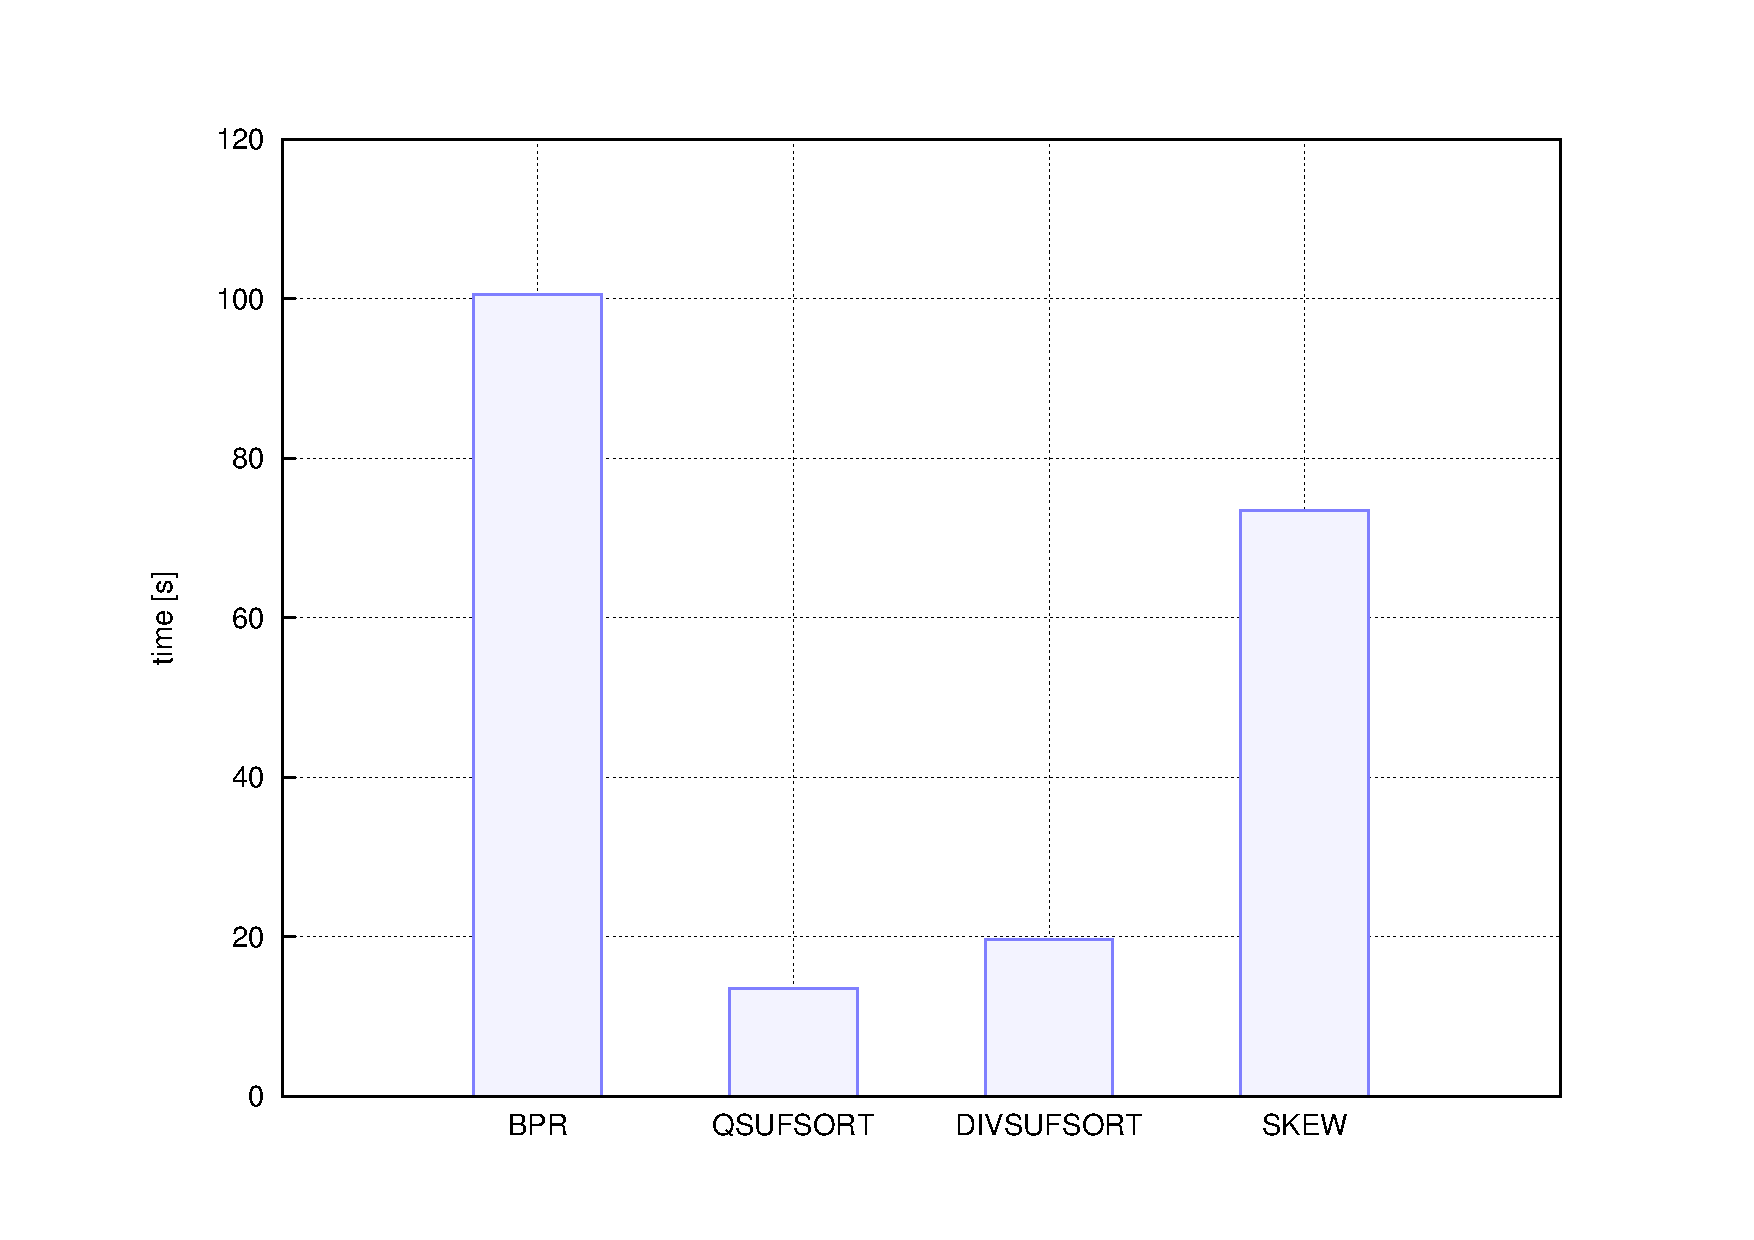
\includegraphics[width=\linewidth]{figures/results/sun-gauntlet.pdf}
    \end{center}        
    \caption{Sumaryczny czas działania algorytmów na plikach z~korpusu \texttt{Gauntlet}.}%
    \label{rys:sun-gauntlet}
\end{figure} 

\begin{table}[ht]
    \begin{center}        
        \begin{tabular}{l r r r r } \toprule
 & \emph{bpr} & \emph{divsufsort} & \emph{qsufsort} & \emph{skew}\\ \midrule
\texttt{chr22.dna} & \textbf{7.93} & 9.15 & 8.38 & 63.94\\
\texttt{etext99} & 32.45 & 32.38 & \textbf{29.48} & ---\\
\texttt{gcc-3.0.tar} & 25.45 & 19.74 & \textbf{16.61} & ---\\
\texttt{howto} & 9.71 & 9.92 & \textbf{8.46} & 82.36\\
\texttt{jdk13c} & 18.77 & 16.84 & \textbf{13.59} & ---\\
\texttt{linux-2.4.5.tar} & 29.32 & 27.61 & \textbf{24.55} & ---\\
\texttt{rctail96} & 35.18 & 32.71 & \textbf{27.64} & ---\\
\texttt{rfc} & 32.69 & 29.21 & \textbf{28.99} & ---\\
\texttt{sprot34.dat} & 32.81 & 31.97 & \textbf{25.60} & ---\\
\texttt{w3c2} & 27.51 & 25.63 & \textbf{20.47} & ---\\
 \midrule
Total & 251.82 & 235.16 & \textbf{203.76} & \\
 \bottomrule
\end{tabular}
 
    \end{center}                         
    \caption{Czas działania algorytmów na plikach z~korpusu Giovanniego Manziniego.}%
    \label{tab:sun-manzini}
\end{table}

\begin{figure}[ht]
   \begin{center}
        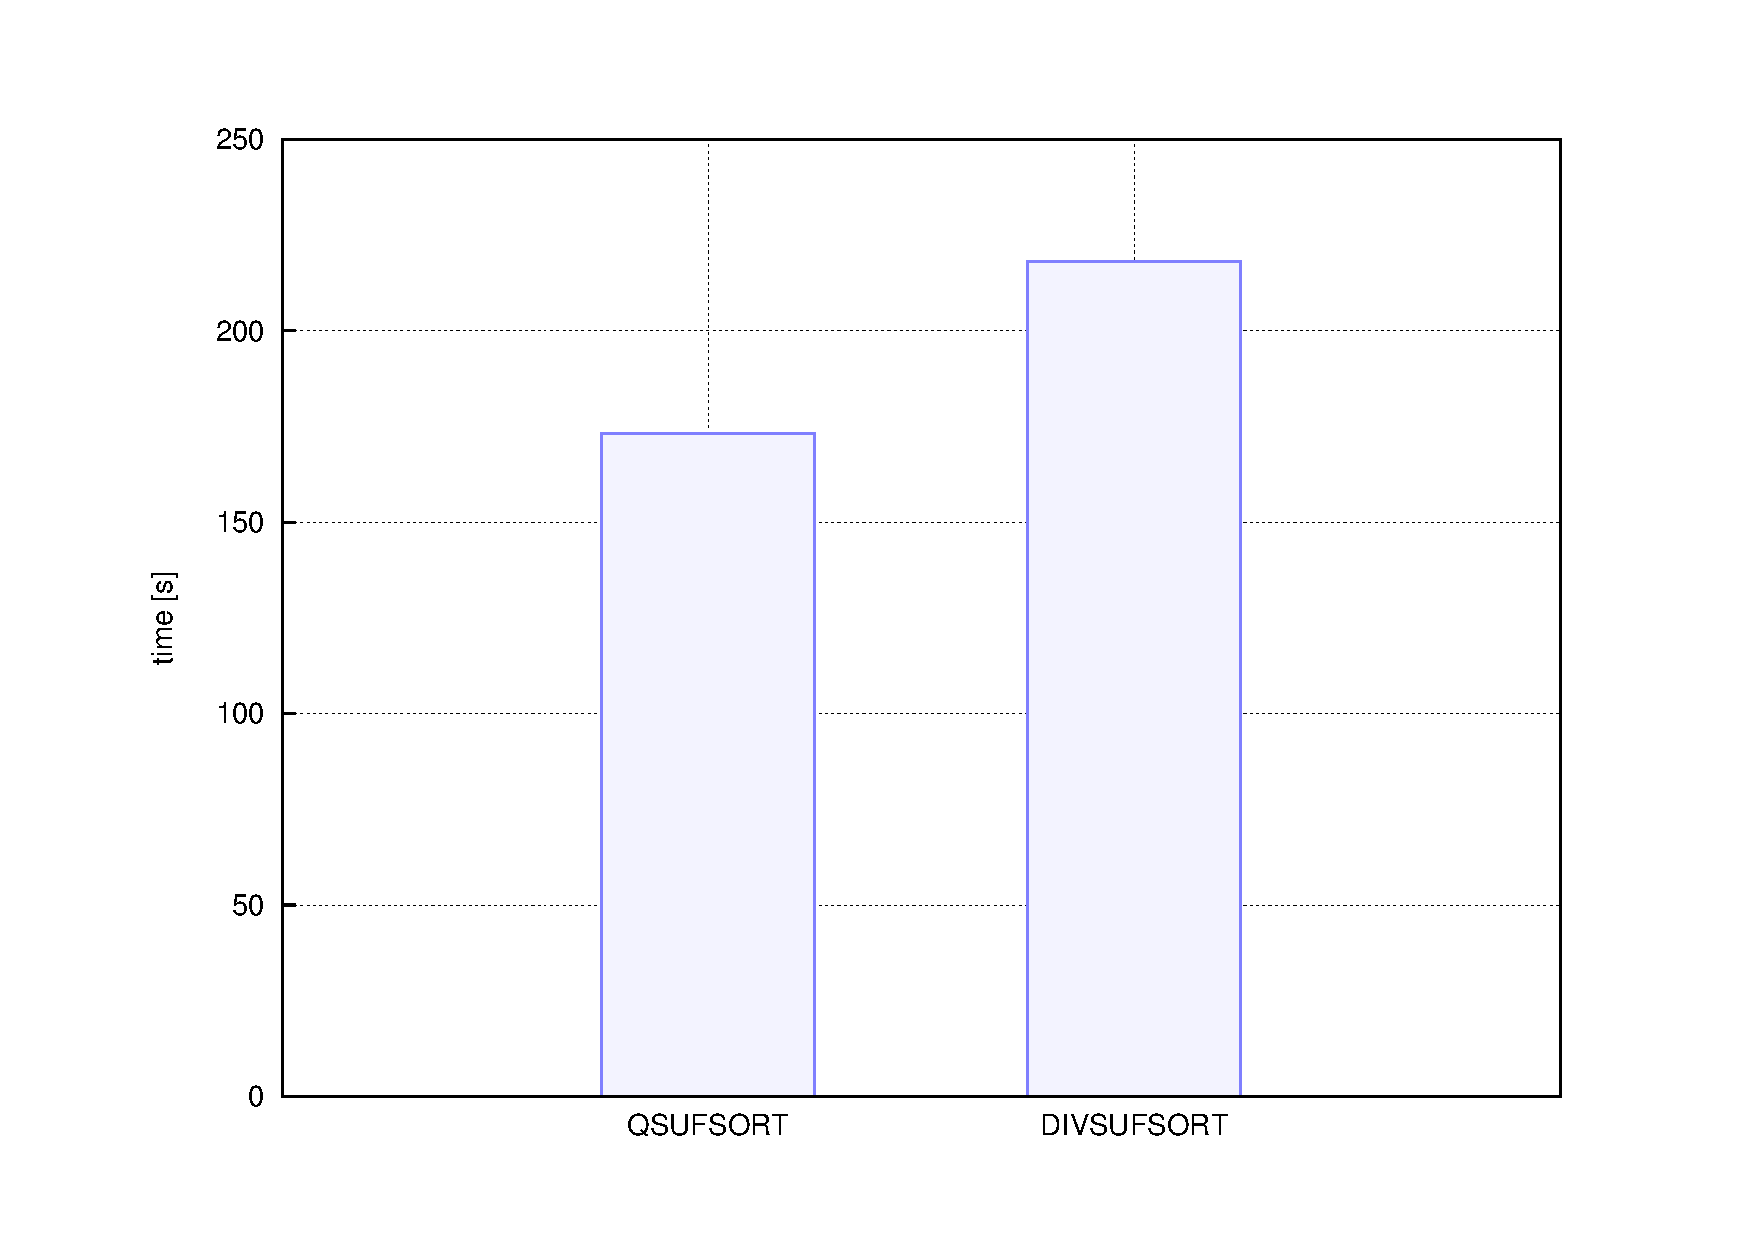
\includegraphics[width=\linewidth]{figures/results/sun-manzini.pdf}
    \end{center}        
    \caption{Sumaryczny czas działania algorytmów na plikach z~korpusu Giovanniego Manziniego.}%
    \label{rys:sun-manzini}
\end{figure} 


\FloatBarrier
\subsection{Porównanie czasów działania algorytmów na różnych maszynach wirtualnych}\label{sect:vms}

Poniżej przedstawione są wyniki podsumowań czasów działania algorytmów na korpusach testowych. Jak
już wspomniano wcześniej, ranking algorytmów jest identyczny dla każdej maszyny wirtualnej. Celem
prezentowania zestawień jest znalezienie takiej maszyny wirtualnej, na której algorytmy działają
najszybciej. Tabele \ref{tab:manzini-vm-compare} i~\ref{tab:gauntlet-vm-compare} zawierają czasy
działań algorytmów na plikach z~korpusów Giovanniego Manziniego i~\texttt{The Gauntlet}. Ze względu
na bardzo niskie wartości odchylenia standardowego nie umieszczono go tabelach. Wizualne porównanie
sum tych wyników znajduje się na rysunkach \ref{rys:manzini-vm-compare}
i~\ref{rys:gauntlet-vm-compare}.
	
Testowane maszyny wirtualne wypadły bardzo podobnie. Na maszynie \texttt{harmony} algorytmy działały
wolniej, wyniki pozostałych trzech maszyn są do siebie zbliżone. Spośród tych wyników wyróżnia się
jednak wynik testu algorytmu \emph{divsufsort} na korpusie Manziniego przeprowadzonego na maszynie
wirtualnej \texttt{jrockit} -- dwukrotnie gorszy niż na pozostałych maszynach. Wyniki w~tabeli
\ref{tab:jrockit-manzini} pokazują wolniejsze działania algorytmu na każdym z~plików wejściowych.
Analiza zapisów przebiegu działania algorytmu wykazała bardzo duże odchylenie standardowe czasu
działania algorytmu, co sugeruje wpływ maszyny wirtualnej (\emph{JIT}, \emph{garbage
collector}) lub jakiś inny proces obliczeniowy działające w tle i~zaburzający pomiar czasu.

\begin{table}[ht]
    \begin{center}        
        \begin{tabular}{l r r r r } \toprule
 & \emph{bpr} & \emph{divsufsort} & \emph{qsufsort} & \emph{skew} \\ \midrule
\texttt{sun} & 100.58 & 19.70 & 13.55 & 73.44 \\
\texttt{ibm} & --- & 18.49 & 14.71 & 71.02 \\
\texttt{jrockit} & 105.05 & 16.49 & 13.55 & 68.24 \\
\texttt{harmony} & 126.39 & 20.85 & 16.51 & 72.53 \\
\bottomrule
\end{tabular}
 
    \end{center}                         
    \caption{Czasy działania algorytmów na korpusie \texttt{Gauntlet} na różnych maszynach wirtualnych. Podane wartości wyrażone są w~sekundach.}
    \label{tab:gauntlet-vm-compare}
\end{table}

\begin{table}[ht]
    \begin{center}        
        \begin{tabular}{l r r r } \toprule
 & \emph{bpr} & \emph{divsufsort} & \emph{qsufsort} \\ \midrule
\texttt{sun} & --- & 218.09 & 173.10  \\
\texttt{ibm} & --- & 212.62 & 179.12 \\
\texttt{jrockit} & 200.84 & 416.30 & 170.00 \\
\texttt{harmony} & 251.82 & 235.16 & 203.76 \\
\bottomrule
\end{tabular}

 
    \end{center}                         
    \caption{Czasy działania algorytmów na korpusie Giovanniego Manziniego na różnych maszynach wirtualnych. Podane wartości wyrażone są w~sekundach.}
    \label{tab:manzini-vm-compare}
\end{table}

% TODO: kolorowe rysunki nie są dobrym pomysłem na wydruk, a te wszystkie kolory są tak samo pastelowe i wyjdą szaro. No
% chyba, że będziesz drukował w kolorze...

\begin{figure}[p]
    \begin{center}
        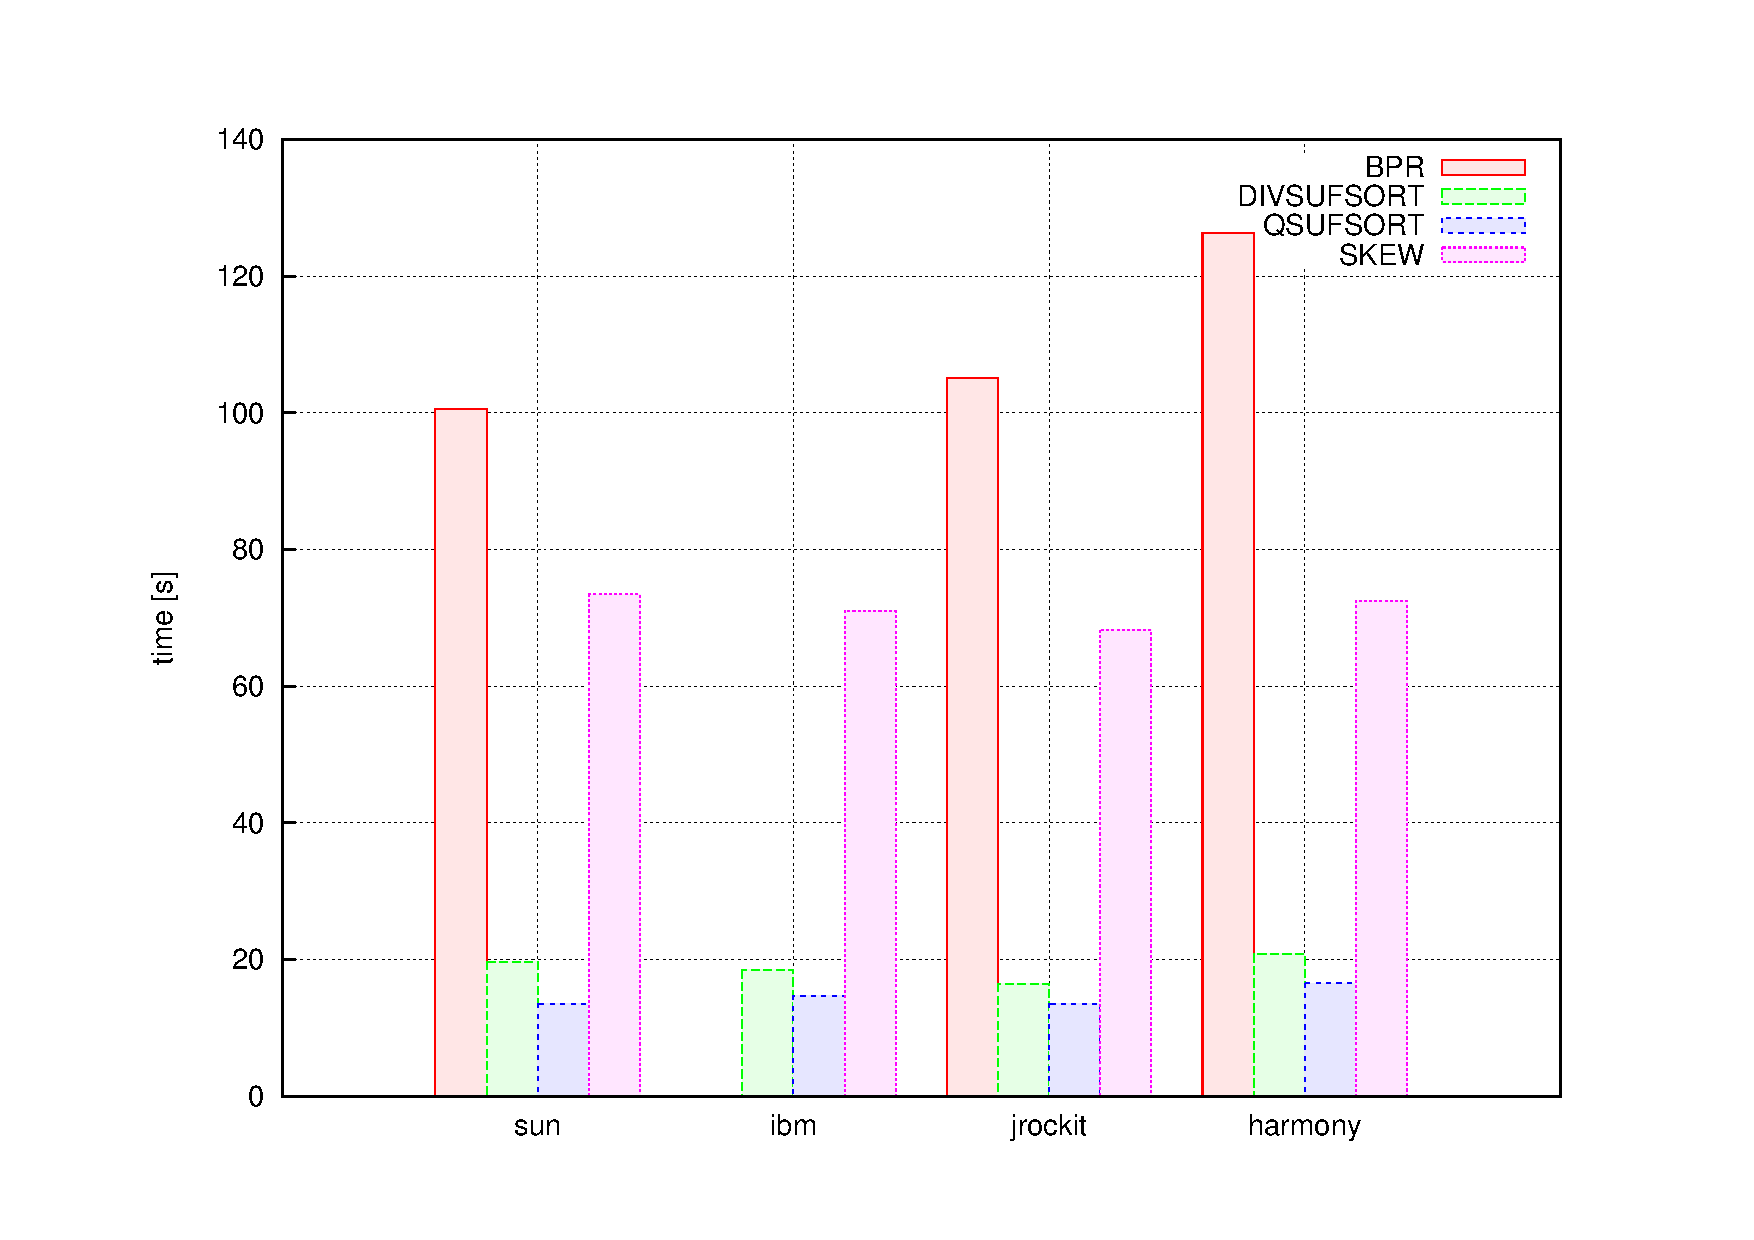
\includegraphics[width=.9\linewidth]{figures/results/gauntlet-compare.pdf}
    \end{center}        
    \caption{Porównanie czasu działania algorytmów na korpusie \texttt{Gauntlet} na różnych maszynach wirtualnych.}
    \label{rys:gauntlet-vm-compare}
\end{figure}

\begin{figure}[p]
    \begin{center}
        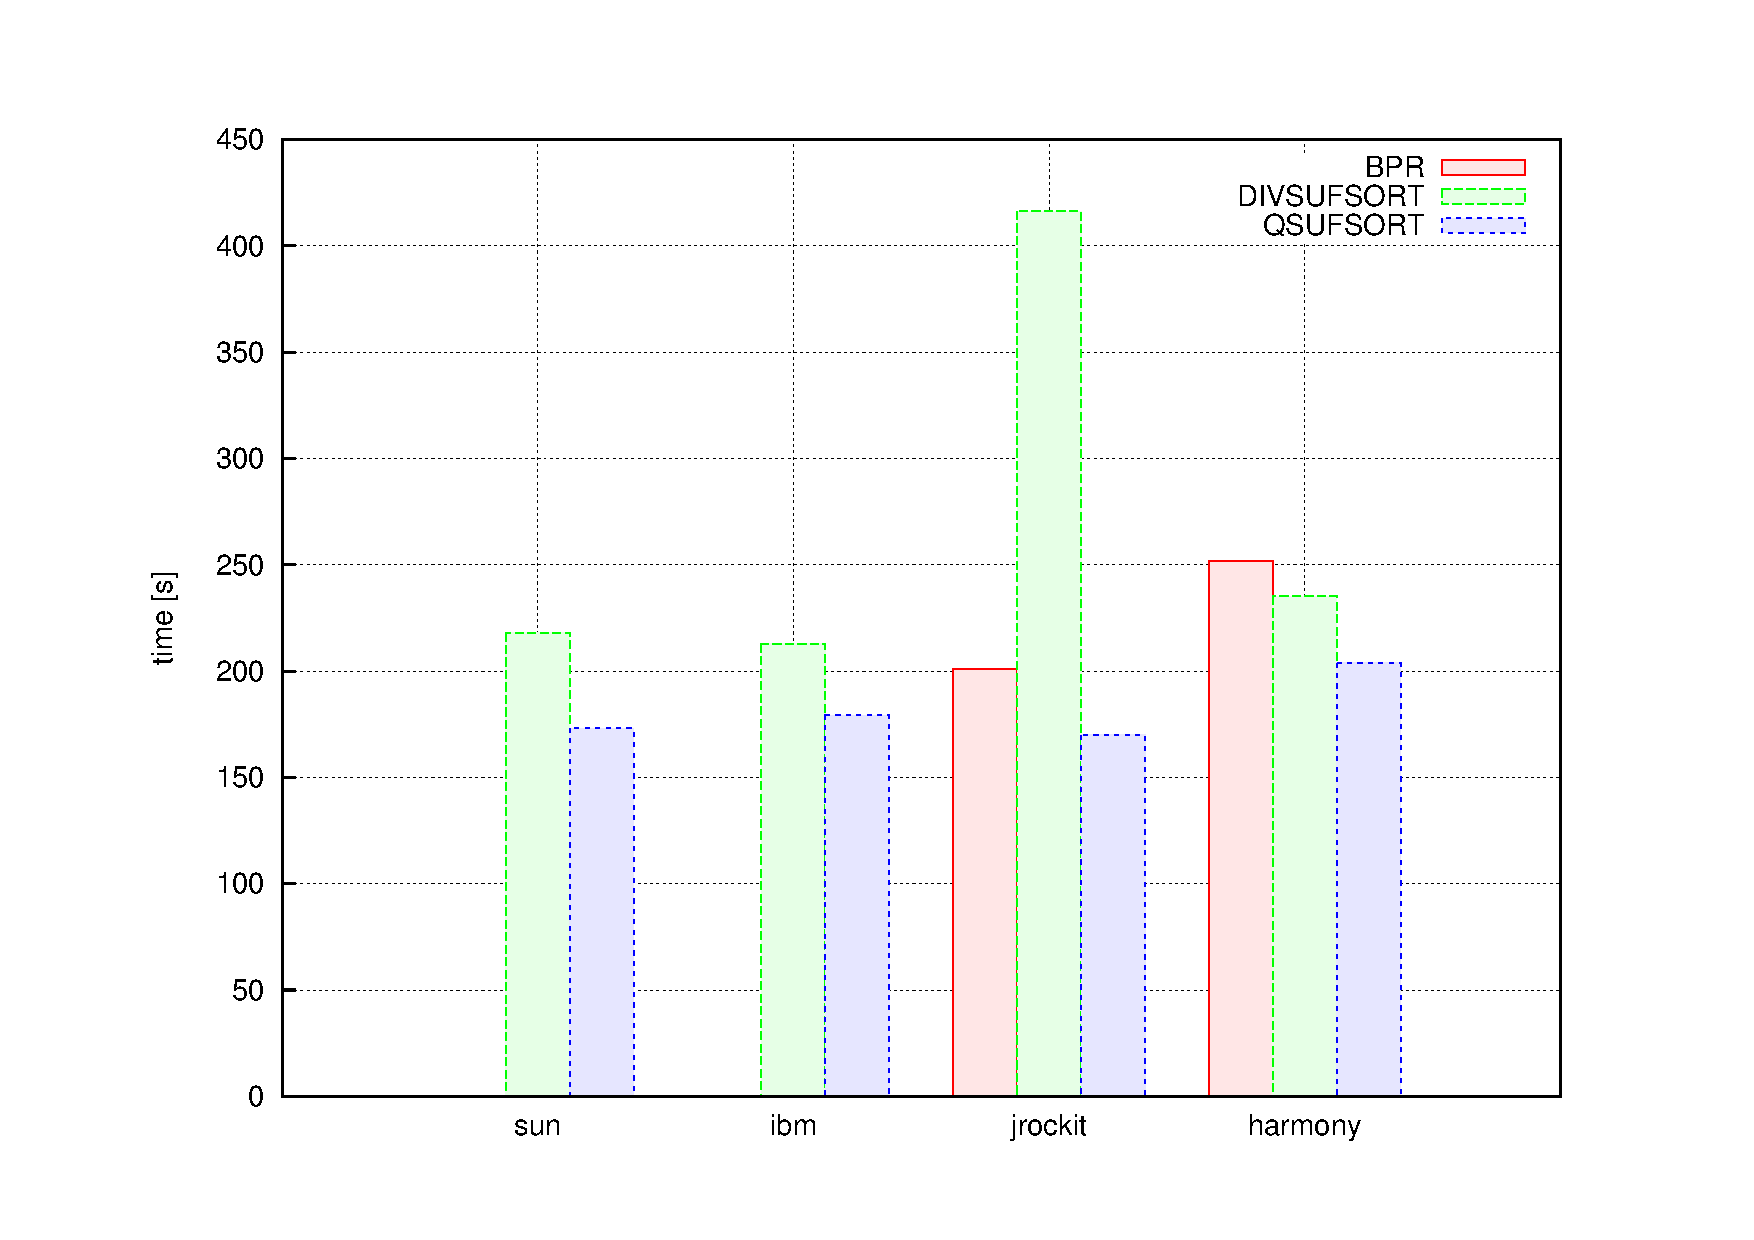
\includegraphics[width=.9\linewidth]{figures/results/manzini-compare.pdf}
        \end{center}        
        \caption{Porównanie czasu działania algorytmów na korpusie Giovanniego Manziniego na różnych maszynach wirtualnych.}
        \label{rys:manzini-vm-compare}
\end{figure}


\FloatBarrier
\section{Analiza wyników}

Najlepszym spośród zaimplementowanych algorytmów okazał się algorytm \emph{qsufsort}. Cechuje się on
odpornością na specyficzne typy danych wejściowych, nie zależy w dużym stopniu ani od rozmiaru
alfabetu sekwencji wejściowej ani od wartości średniego \emph{lcp}. Dodatkowym atutem jest brak
użycia dodatkowej pamięci ponad tą wymaganą do przechowania wejścia i~wyjścia algorytmu (oraz stosu
zużytego podczas rekurencyjnego sortowania). Na drugim miejscu znalazł się algorytm
\emph{divsufsort} ustępujący zwycięzcy zarówno pod względem czasu działania, jak i~zużycia pamięci.
Pozostałe algorytmy wypadły dużo gorzej niż wymieniona dwójka.

Co ciekawe, publikowane w~internecie wyniki testów wydajnościowych implementacji algorytmów w~języku
\texttt{C++} [\ref{msufsort}, \ref{mori-benchmark}] dają nieco inny obraz rankingu tych algorytmów.
Najlepsze wyniki uzyskują tam implementacje algorytmu \emph{improved two-stage}, czyli
\emph{archon}, \emph{divsufsort} i~\emph{msufsort}. Algorytm \emph{qsufsort} uzyskuje dobre, choć
wyraźnie gorsze wyniki. Wytłumaczenie przyczyn tego faktu leży zapewne w~różnicach między językami
\texttt{C++} a~\texttt{Java} (oraz działaniem kodu natywnego i~kodu uruchamianego na maszynie
wirtualnej). Algorytm \emph{qsufsort} jest prostym algorytmem, zarówno koncepcyjnie jak
i~implementacyjnie. Przepisanie go z~\texttt{C++} do \texttt{Javy} nie było trudne. Algorytm
\emph{divsufsort} jest dużo bardziej złożony (jego implementacja w~języku \texttt{Java} jest o~ponad
2000 linii kodu dłuższa od \emph{qsufsort}). Z~powodu wykorzystywania wskaźników oraz instrukcji
\texttt{\#define} w~oryginalnej implementacji, kod w~języku \texttt{Java} różni się od oryginału
w~wielu miejscach. Wydaje się, że dominujące dla szybkości działania różnice to:
\begin{itemize}
    \item allokacja złożonych struktur danych (i tablic lokalnych) następuję w języku \texttt{Java}
    na stercie, a nie na stosie; oprócz samego narzutu allokacji dochodzi tu również koszt 
    procesu oczyszczania pamięci (\emph{garbage collector});
    
    \item wskaźniki z języków niskopoziomowych muszą być modelowane jako indeksy nad tablicami typów prostych, 
    co w języku \texttt{Java} wiąże się z dodatkowym narzutem sprawdzenia czy indeks nie przekracza
    rozmiaru tablicy;

    \item rozmiar kodu natywnego generowanego dynamicznie w języku \texttt{Java} prawdopodobnie przekraczał wielokrotnie
    rozmiar kodu skompilowanego w języku \texttt{C}, powodując gorsze użytkowanie pamięci podręcznej
    procesora.
\end{itemize}

Algorytm \emph{skew} jako jedyny spośród testowanych algorytmów posiadał liniową teoretyczną złożoność
obliczeniową. W~testach wydajnościowych wypadł jednak bardzo słabo, zarówno w~testach implementacji
w~języku \texttt{Java}, jak i~w~języku \texttt{C++}. Przyczyną takiego zachowania algorytmu jest
jego bardzo duża złożoność pamięciowa zwiększana dodatkowo przez rekurencyjne wywoływanie algorytmu.
Ponadto, rekurencja wiąże się z~dodatkowymi kosztami związanymi z~obsługą stosu. Należy również
pamiętać, że podane złożoności pozostałych algorytmów są wartościami pesymistycznymi, które są
rzadko osiągane w praktyce.



\chapter{Podsumowanie i kierunki dalszego rozwoju}

Nadrzędnym celem niniejszej pracy było napisanie (w formie biblioteki) implementacji wybranych
algorytmów tworzenia tablic sufiksów w celu analizy ich efektywności i zachowania w języku wysokiego
poziomu, jakim jest język \texttt{Java}. Zadanie to obejmowało zapoznanie się z~dostępną literaturą
poświęconą tematyce tablic sufiksów, wybór najciekawszych algorytmów oraz ich opisanie. Dodatkowo,
w~wyniku pracy powinna była powstać klasyfikacja algorytmów tworzenia tablic sufiksów.

Największym wyzwaniem podczas tworzenia pracy było znalezienie najlepszych spośród algorytmów
tworzenia tablic sufiksów. Bardzo pomocne były w~tym opracowania zawierające zestawienia algorytmów
\cite{taxonomy, schurmann-phd} oraz publikowane w~internecie wyniki testów wydajnościowych
[\ref{msufsort}, \ref{mori-benchmark}]. Pewnym problemem podczas implementacji algorytmów było tłumaczenie
do języka \texttt{Java} takich konstrukcji języka \texttt{C++}, jak instrukcje \texttt{define},
wskaźniki oraz inne polecenia preprocesora.

Podsumowując, należy stwierdzić, że wszystkie zakładane cele zostały zrealizowane. Przegląd
literatury, opisy algorytmów oraz ich klasyfikacja znalazły się w~tekście tej pracy, podobnie jak
wyniki testów wydajnościowych powstałej implementacji. Według naszej wiedzy niniejsza praca jest
pierwszą publikacją w~języku polskim poświęconą w całości tematyce algorytmów tworzenia tablic
sufiksów. Zaimplementowana biblioteka programowa jest zaś na dzień dzisiejszy jedyną taką pozycją
dedykowaną algorytmom tworzenia tablic sufiksów napisaną w~języku \texttt{Java}. Kod źródłowy
biblioteki jest udostępniony na licencji BSD, można go pobrać ze strony projektu:
\url{http://www.jsuffixarrays.org}.

Przewidywany dalszy rozwój biblioteki zakłada opracowanie algorytmu dobierającego najlepszą metodę
tworzenia tablic sufiksów na podstawie charakterystyki danych wejściowych (rozmiaru alfabetu i
rozkładu symboli w danych wejściowych). Interesującym kierunkiem rozwoju biblioteki jest również
stworzenie własnej implementacji algorytmu \emph{improved two-stage}, dostosowanej do specyfiki
języka \texttt{Java}.




% All appendices and extra material, if you have any.
\cleardoublepage\appendix%

\chapter{Wyniki dla pozostałych maszyn wirtualnych}

\begin{table}[p]
	\begin{center}        
 		\begin{tabular}{l r r r r } \toprule
 & \emph{bpr} & \emph{divsufsort} & \emph{qsufsort} & \emph{skew}\\ \midrule
\texttt{abac} & 1.04 & 0.01 & \textbf{0.01} & 0.05\\
\texttt{abba} & 4.23 & \textbf{2.19} & 2.26 & 11.23\\
\texttt{book1x20} & \textbf{3.14} & 3.29 & 3.40 & 22.52\\
\texttt{fib\_s14930352} & 10.05 & 4.94 & \textbf{3.32} & 14.09\\
\texttt{fss10} & 5.36 & 3.88 & \textbf{2.69} & 12.34\\
\texttt{fss9} & 1.05 & 0.63 & \textbf{0.58} & 1.89\\
\texttt{houston} & 2.63 & \textbf{0.24} & 0.44 & 0.96\\
\texttt{paper5x80} & 0.18 & 0.15 & \textbf{0.08} & 0.42\\
\texttt{test1} & 2.26 & 0.41 & \textbf{0.20} & 1.91\\
\texttt{test2} & 0.71 & 0.34 & \textbf{0.20} & 1.91\\
\texttt{test3} & 74.40 & 0.42 & \textbf{0.37} & 0.91\\
 \midrule
Total & 105.05 & 16.49 & \textbf{13.55} & 68.24\\
 \bottomrule
\end{tabular}

    \end{center}                         
	\caption{Czas działania algorytmów na plikach z korpusu \texttt{The Gauntlet} dla maszyny wirtualnej \texttt{ibm}.}%
    \label{tab:ibm-gauntlet}
\end{table}

\begin{figure}[p]
   \begin{center}
        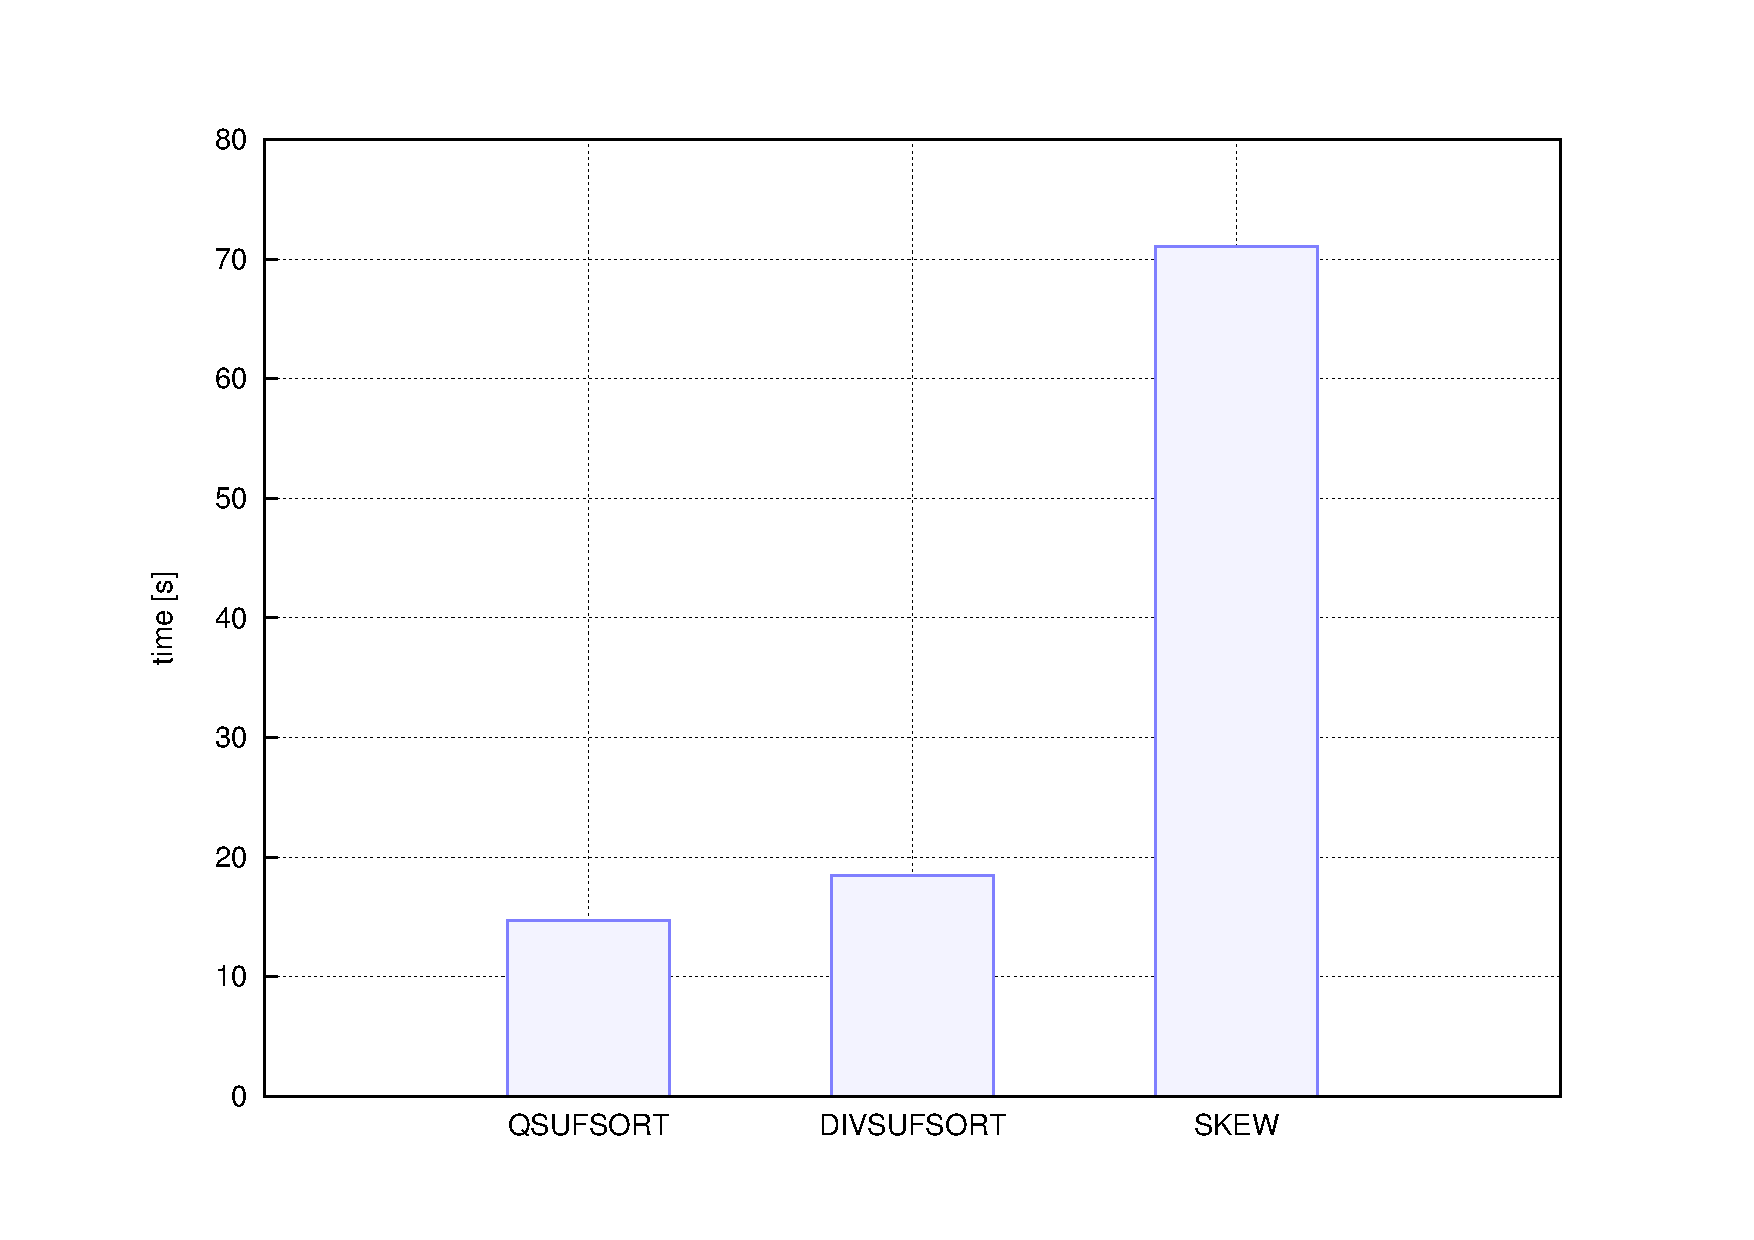
\includegraphics[width=\linewidth]{figures/results/ibm-gauntlet.pdf}
    \end{center}        
    \caption{Sumaryczny czas działania algorytmów na plikach z korpusu \texttt{The Gauntlet} dla maszyny wirtualnej \texttt{ibm}.}%
    \label{rys:ibm-gauntlet}
\end{figure}


\begin{table}[p]
	\begin{center}        
 		\begin{tabular}{l r r r r } \toprule
 & \emph{bpr} & \emph{divsufsort} & \emph{qsufsort} & \emph{skew}\\ \midrule
\texttt{chr22.dna} & \textbf{7.93} & 9.15 & 8.38 & 63.94\\
\texttt{etext99} & 32.45 & 32.38 & \textbf{29.48} & ---\\
\texttt{gcc-3.0.tar} & 25.45 & 19.74 & \textbf{16.61} & ---\\
\texttt{howto} & 9.71 & 9.92 & \textbf{8.46} & 82.36\\
\texttt{jdk13c} & 18.77 & 16.84 & \textbf{13.59} & ---\\
\texttt{linux-2.4.5.tar} & 29.32 & 27.61 & \textbf{24.55} & ---\\
\texttt{rctail96} & 35.18 & 32.71 & \textbf{27.64} & ---\\
\texttt{rfc} & 32.69 & 29.21 & \textbf{28.99} & ---\\
\texttt{sprot34.dat} & 32.81 & 31.97 & \textbf{25.60} & ---\\
\texttt{w3c2} & 27.51 & 25.63 & \textbf{20.47} & ---\\
 \midrule
Total & 251.82 & 235.16 & \textbf{203.76} & \\
 \bottomrule
\end{tabular}
 
    \end{center}                         
	\caption{Czas działania algorytmów na plikach z korpusu Giovanniego Manziniego dla maszyny wirtualnej \texttt{ibm}.}%
    \label{tab:ibm-manzini}
\end{table}

\begin{figure}[p]
       \begin{center}
            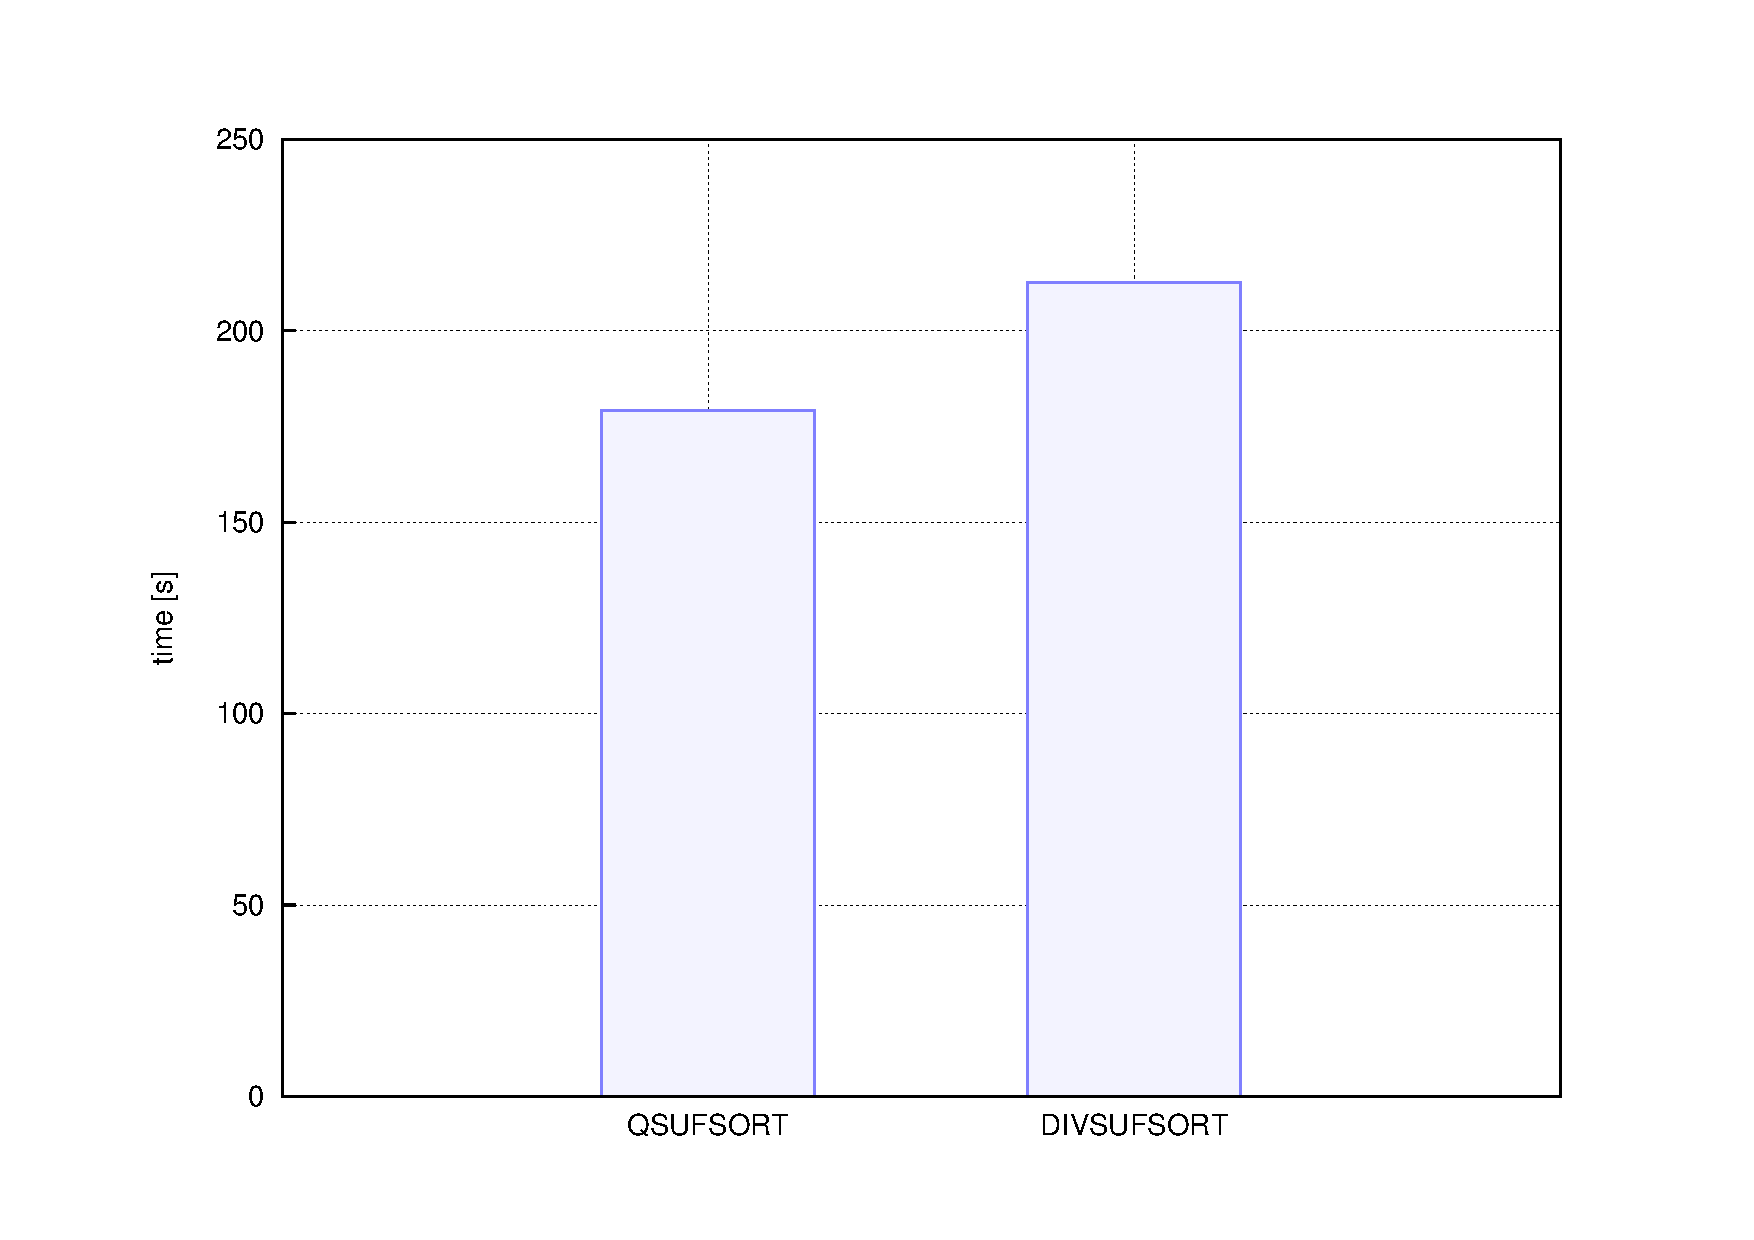
\includegraphics[width=\linewidth]{figures/results/ibm-manzini.pdf}
        \end{center}        
	    \caption{Sumaryczny czas działania algorytmów na plikach z korpusu Giovanniego Manziniego dla maszyny wirtualnej \texttt{ibm}.}%
    \label{rys:ibm-manzini}
\end{figure}
 

\begin{table}[p]
	\begin{center}        
 		\begin{tabular}{l r r r r } \toprule
 & \emph{bpr} & \emph{divsufsort} & \emph{qsufsort} & \emph{skew}\\ \midrule
\texttt{abac} & 1.04 & 0.01 & \textbf{0.01} & 0.05\\
\texttt{abba} & 4.23 & \textbf{2.19} & 2.26 & 11.23\\
\texttt{book1x20} & \textbf{3.14} & 3.29 & 3.40 & 22.52\\
\texttt{fib\_s14930352} & 10.05 & 4.94 & \textbf{3.32} & 14.09\\
\texttt{fss10} & 5.36 & 3.88 & \textbf{2.69} & 12.34\\
\texttt{fss9} & 1.05 & 0.63 & \textbf{0.58} & 1.89\\
\texttt{houston} & 2.63 & \textbf{0.24} & 0.44 & 0.96\\
\texttt{paper5x80} & 0.18 & 0.15 & \textbf{0.08} & 0.42\\
\texttt{test1} & 2.26 & 0.41 & \textbf{0.20} & 1.91\\
\texttt{test2} & 0.71 & 0.34 & \textbf{0.20} & 1.91\\
\texttt{test3} & 74.40 & 0.42 & \textbf{0.37} & 0.91\\
 \midrule
Total & 105.05 & 16.49 & \textbf{13.55} & 68.24\\
 \bottomrule
\end{tabular}

    \end{center}                         
	\caption{Czas działania algorytmów na plikach z korpusu \texttt{The Gauntlet} dla maszyny wirtualnej \texttt{jrockit}.}%
    \label{tab:jrockit-gauntlet}
\end{table}

\begin{figure}[p]
       \begin{center}
            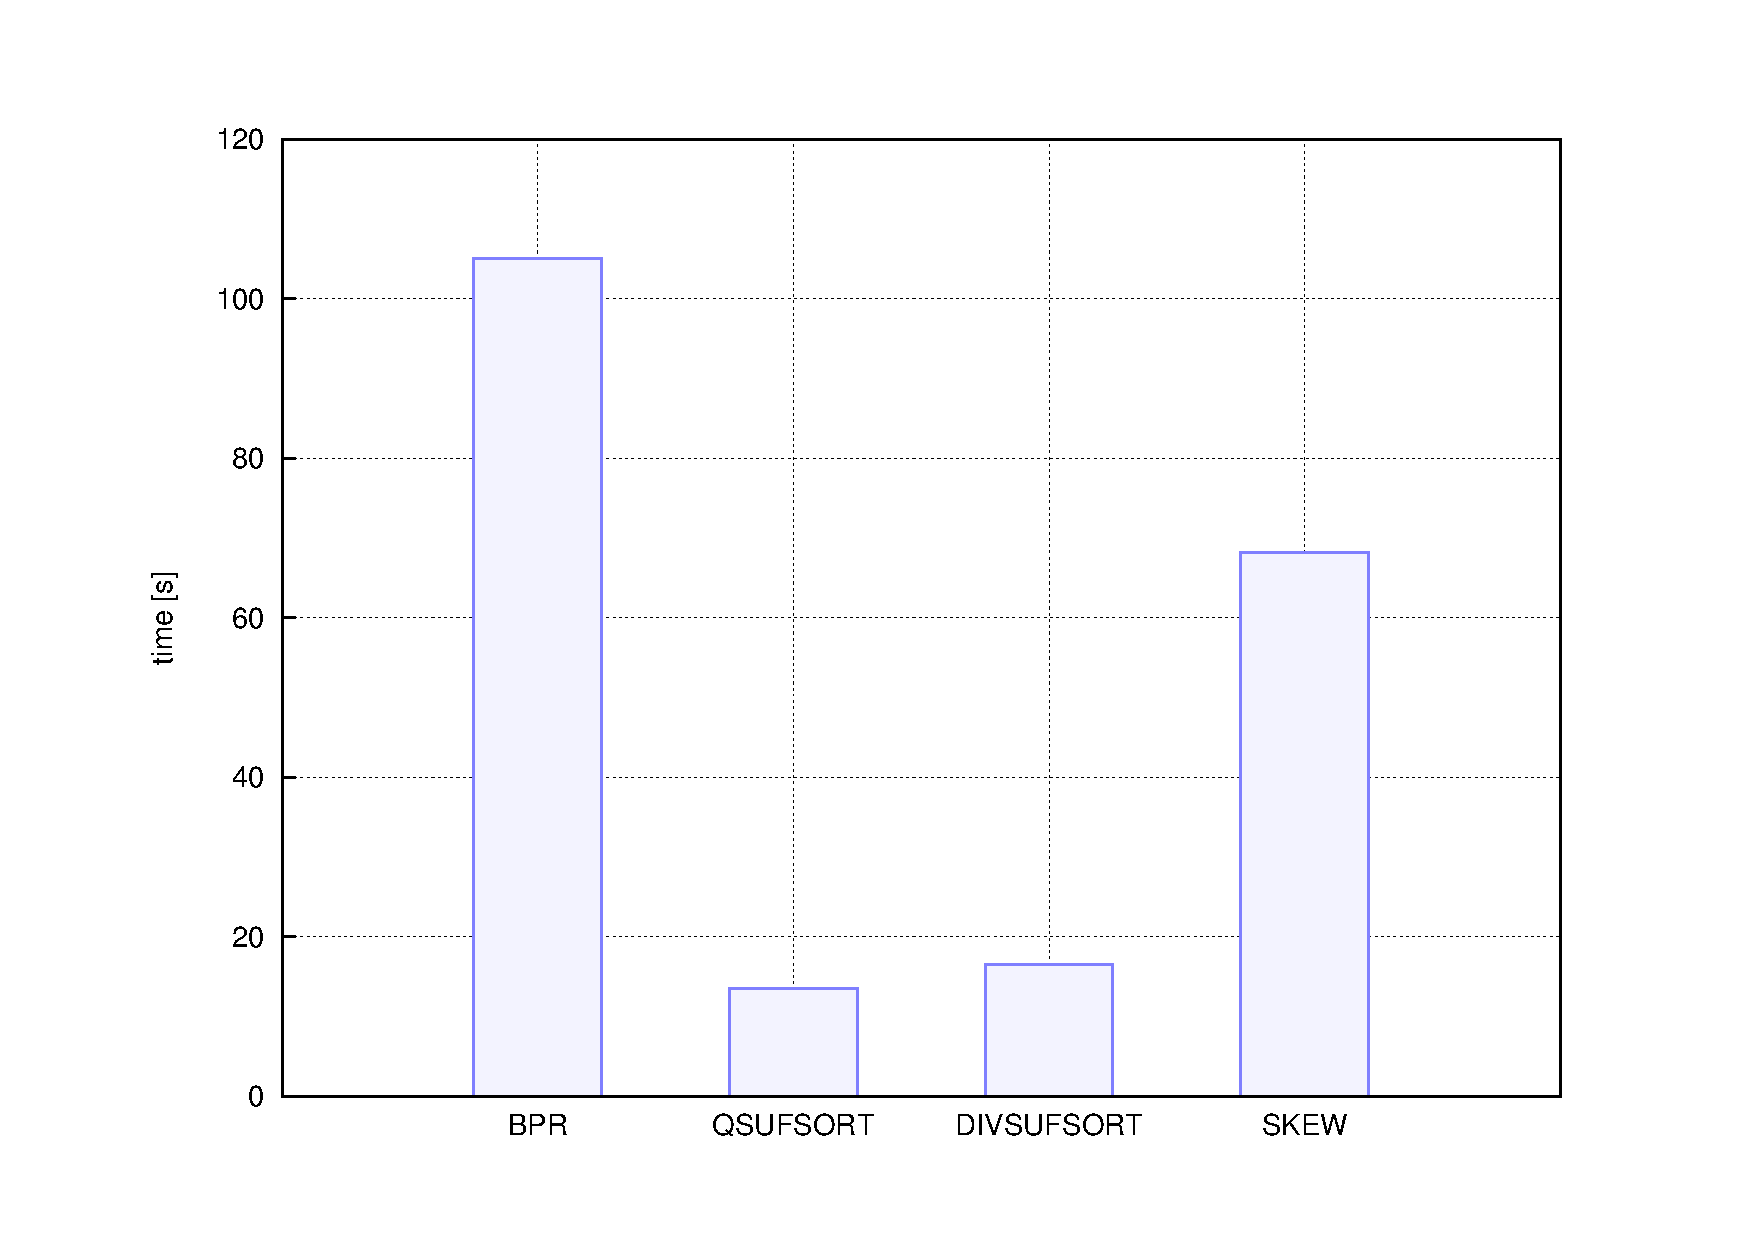
\includegraphics[width=\linewidth]{figures/results/jrockit-gauntlet.pdf}
        \end{center}        
	    \caption{Sumaryczny czas działania algorytmów na plikach z korpusu \texttt{The Gauntlet} dla maszyny wirtualnej \texttt{jrockit}.}%
    \label{rys:jrockit-gauntlet}
\end{figure} 


\begin{table}[p]
	\begin{center}        
 		\begin{tabular}{l r r r r } \toprule
 & \emph{bpr} & \emph{divsufsort} & \emph{qsufsort} & \emph{skew}\\ \midrule
\texttt{chr22.dna} & \textbf{7.93} & 9.15 & 8.38 & 63.94\\
\texttt{etext99} & 32.45 & 32.38 & \textbf{29.48} & ---\\
\texttt{gcc-3.0.tar} & 25.45 & 19.74 & \textbf{16.61} & ---\\
\texttt{howto} & 9.71 & 9.92 & \textbf{8.46} & 82.36\\
\texttt{jdk13c} & 18.77 & 16.84 & \textbf{13.59} & ---\\
\texttt{linux-2.4.5.tar} & 29.32 & 27.61 & \textbf{24.55} & ---\\
\texttt{rctail96} & 35.18 & 32.71 & \textbf{27.64} & ---\\
\texttt{rfc} & 32.69 & 29.21 & \textbf{28.99} & ---\\
\texttt{sprot34.dat} & 32.81 & 31.97 & \textbf{25.60} & ---\\
\texttt{w3c2} & 27.51 & 25.63 & \textbf{20.47} & ---\\
 \midrule
Total & 251.82 & 235.16 & \textbf{203.76} & \\
 \bottomrule
\end{tabular}
 
    \end{center}                         
\caption{Czas działania algorytmów na plikach z korpusu Giovanniego Manziniego dla maszyny wirtualnej \texttt{jrockit}.}%
    \label{tab:jrockit-manzini}
\end{table}

\begin{figure}[p]
       \begin{center}
            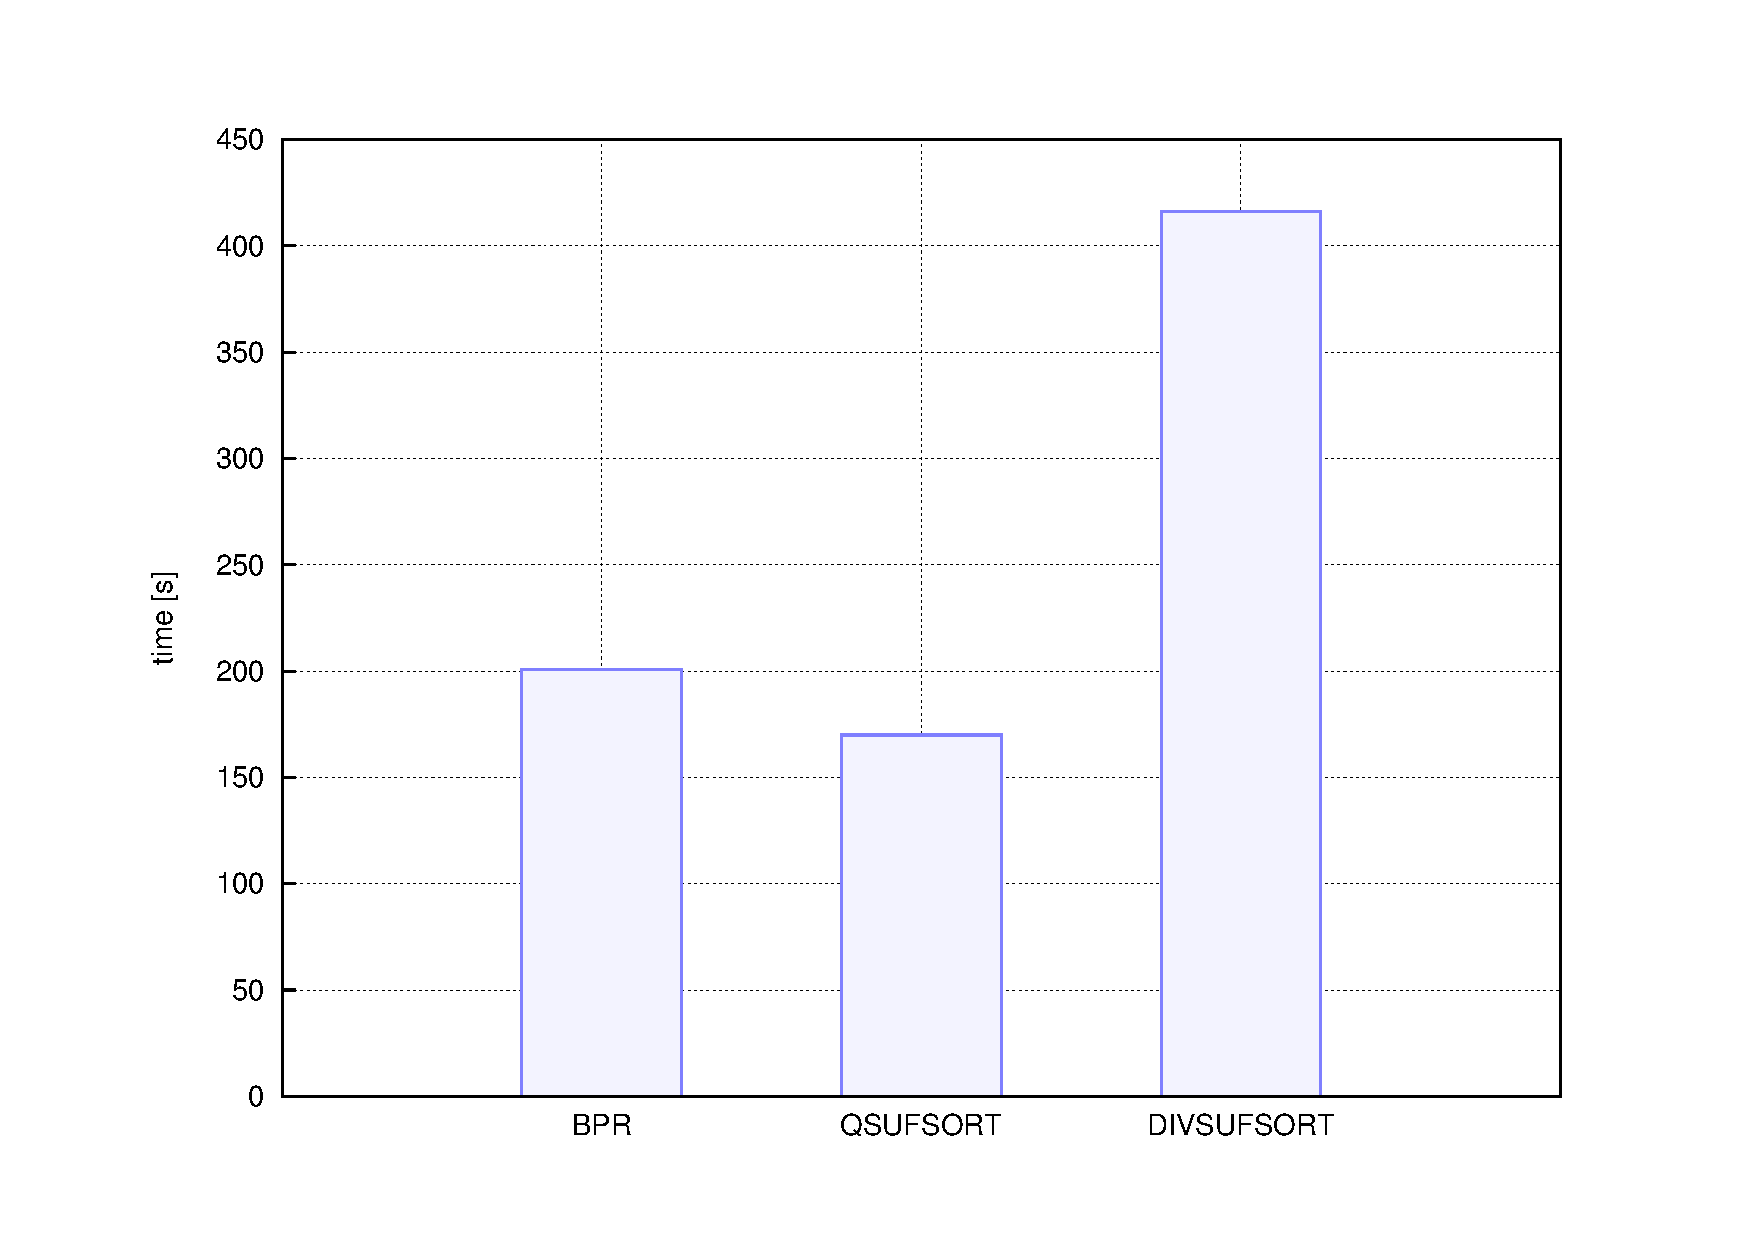
\includegraphics[width=\linewidth]{figures/results/jrockit-manzini.pdf}
        \end{center}        
	    \caption{Sumaryczny czas działania algorytmów na plikach z korpusu Giovanniego Manziniego dla maszyny wirtualnej \texttt{jrockit}.}%
    \label{rys:jrockit-manzini}
\end{figure} 


\begin{table}[p]
	\begin{center}        
 		\begin{tabular}{l r r r r } \toprule
 & \emph{bpr} & \emph{divsufsort} & \emph{qsufsort} & \emph{skew}\\ \midrule
\texttt{abac} & 1.04 & 0.01 & \textbf{0.01} & 0.05\\
\texttt{abba} & 4.23 & \textbf{2.19} & 2.26 & 11.23\\
\texttt{book1x20} & \textbf{3.14} & 3.29 & 3.40 & 22.52\\
\texttt{fib\_s14930352} & 10.05 & 4.94 & \textbf{3.32} & 14.09\\
\texttt{fss10} & 5.36 & 3.88 & \textbf{2.69} & 12.34\\
\texttt{fss9} & 1.05 & 0.63 & \textbf{0.58} & 1.89\\
\texttt{houston} & 2.63 & \textbf{0.24} & 0.44 & 0.96\\
\texttt{paper5x80} & 0.18 & 0.15 & \textbf{0.08} & 0.42\\
\texttt{test1} & 2.26 & 0.41 & \textbf{0.20} & 1.91\\
\texttt{test2} & 0.71 & 0.34 & \textbf{0.20} & 1.91\\
\texttt{test3} & 74.40 & 0.42 & \textbf{0.37} & 0.91\\
 \midrule
Total & 105.05 & 16.49 & \textbf{13.55} & 68.24\\
 \bottomrule
\end{tabular}

    \end{center}                         
	\caption{Czas działania algorytmów na plikach z korpusu \texttt{The Gauntlet} dla maszyny wirtualnej \texttt{harmony}.}%
    \label{tab:harmony-gauntlet}
\end{table}

\begin{figure}[p]
       \begin{center}
            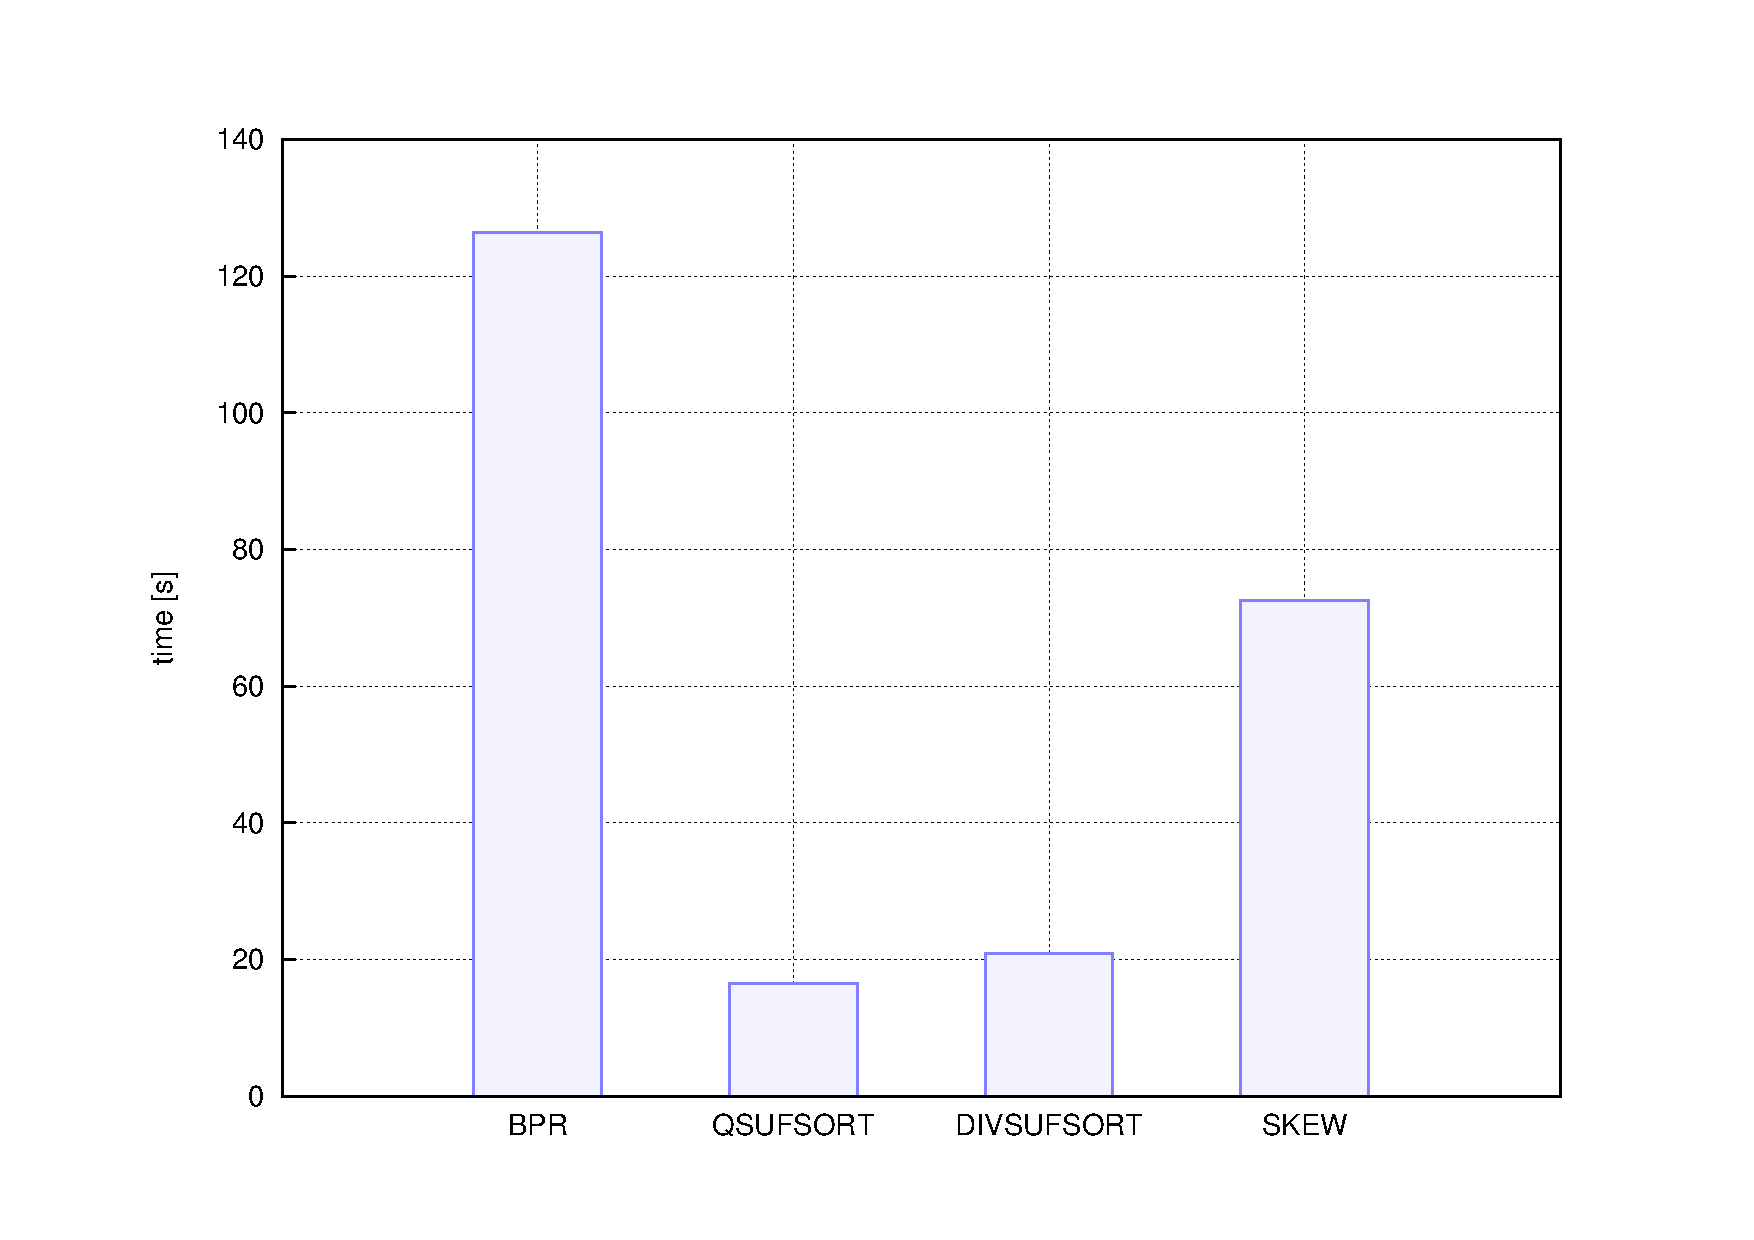
\includegraphics[width=\linewidth]{figures/results/harmony-gauntlet.pdf}
        \end{center}        
	    \caption{Sumaryczny czas działania algorytmów na plikach z korpusu \texttt{The Gauntlet} dla maszyny wirtualnej \texttt{harmony}.}%
    \label{rys:harmony-gauntlet}
\end{figure} 


\begin{table}[p]
	\begin{center}        
 		\begin{tabular}{l r r r r } \toprule
 & \emph{bpr} & \emph{divsufsort} & \emph{qsufsort} & \emph{skew}\\ \midrule
\texttt{chr22.dna} & \textbf{7.93} & 9.15 & 8.38 & 63.94\\
\texttt{etext99} & 32.45 & 32.38 & \textbf{29.48} & ---\\
\texttt{gcc-3.0.tar} & 25.45 & 19.74 & \textbf{16.61} & ---\\
\texttt{howto} & 9.71 & 9.92 & \textbf{8.46} & 82.36\\
\texttt{jdk13c} & 18.77 & 16.84 & \textbf{13.59} & ---\\
\texttt{linux-2.4.5.tar} & 29.32 & 27.61 & \textbf{24.55} & ---\\
\texttt{rctail96} & 35.18 & 32.71 & \textbf{27.64} & ---\\
\texttt{rfc} & 32.69 & 29.21 & \textbf{28.99} & ---\\
\texttt{sprot34.dat} & 32.81 & 31.97 & \textbf{25.60} & ---\\
\texttt{w3c2} & 27.51 & 25.63 & \textbf{20.47} & ---\\
 \midrule
Total & 251.82 & 235.16 & \textbf{203.76} & \\
 \bottomrule
\end{tabular}
 
    \end{center}                         
	\caption{Czas działania algorytmów na plikach z korpusu Giovanniego Manziniego dla maszyny wirtualnej \texttt{harmony}.}%
    \label{tab:harmony-manzini}
\end{table}

\begin{figure}[p]
       \begin{center}
            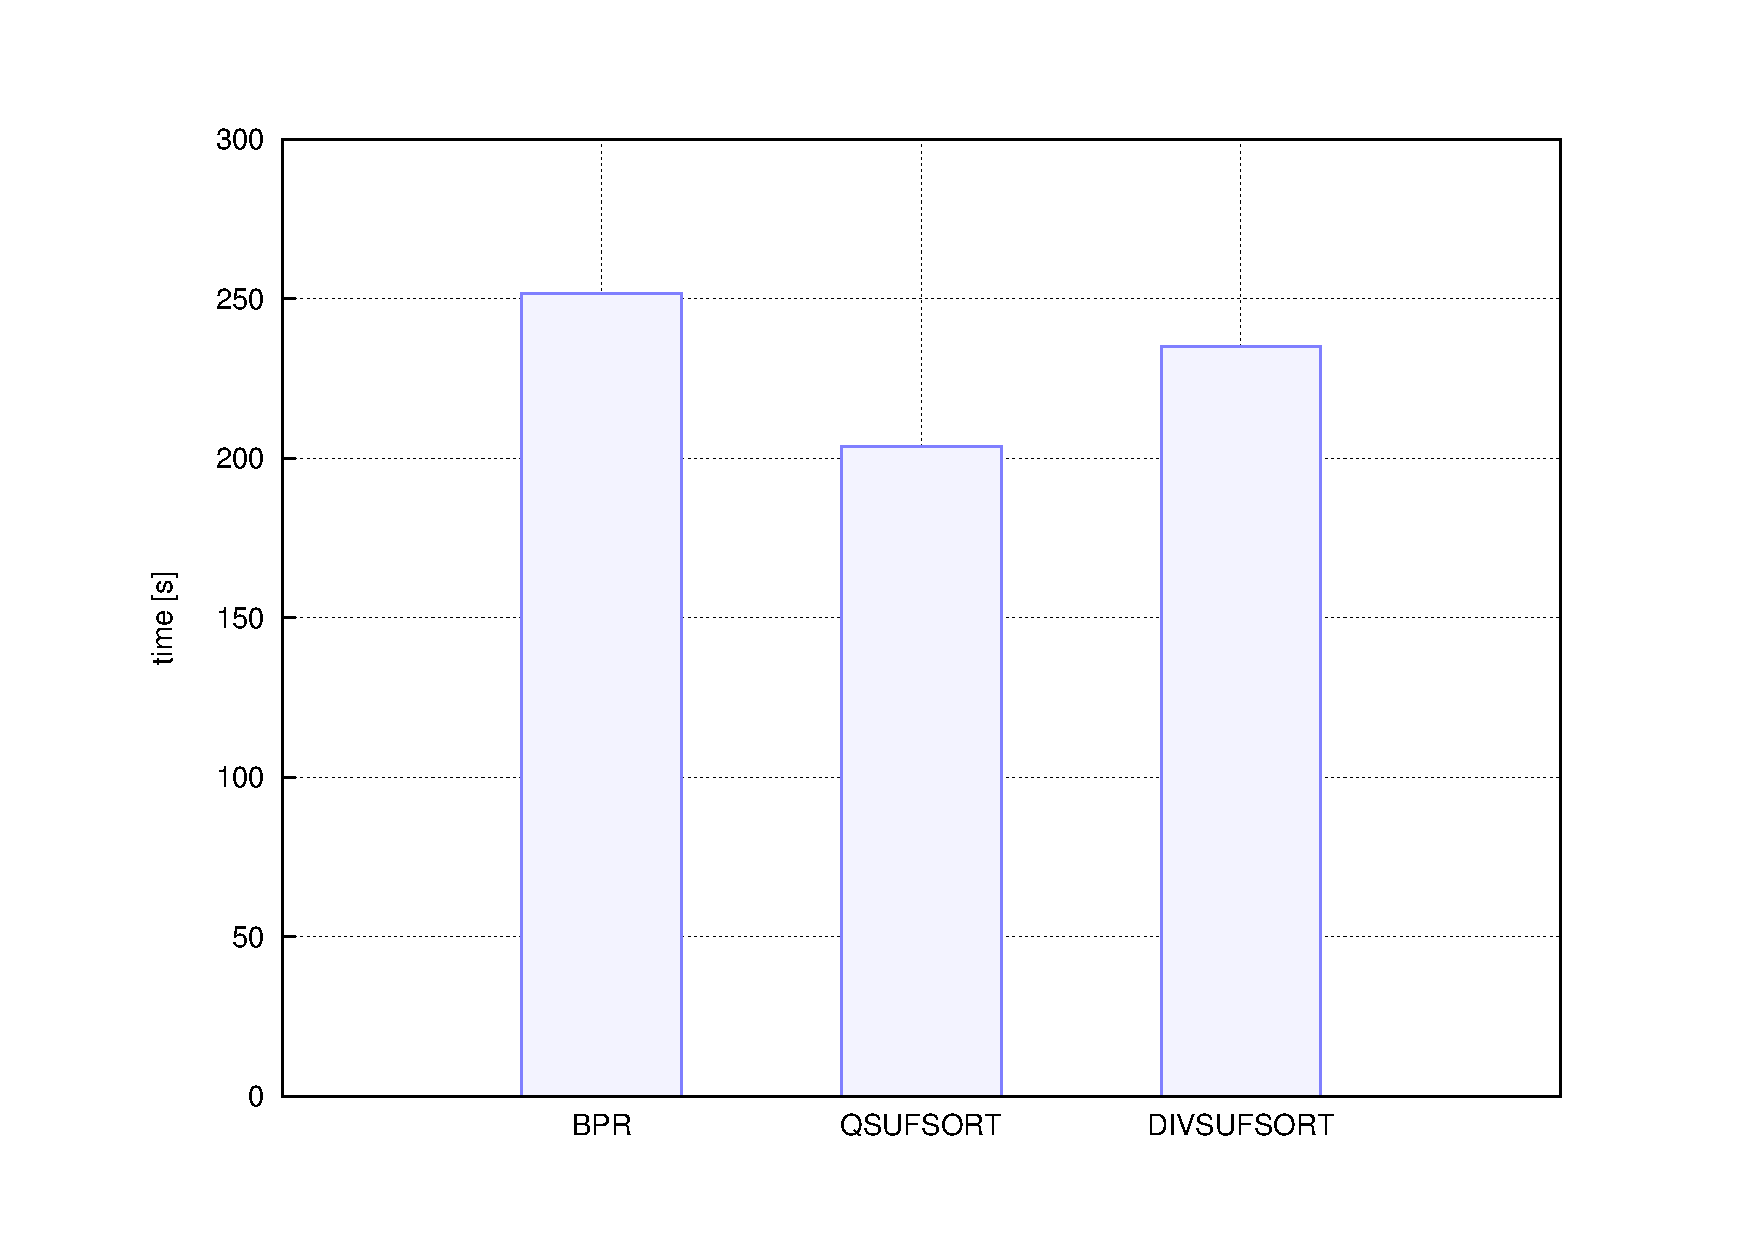
\includegraphics[width=\linewidth]{figures/results/harmony-manzini.pdf}
        \end{center}        
	    \caption{Sumaryczny czas działania algorytmów na plikach z korpusu Giovanniego Manziniego dla maszyny wirtualnej \texttt{harmony}.}%
    \label{rys:harmony-manzini}
\end{figure}
 

% Bibliography (books, articles) starts here.
\bibliographystyle{plalpha}{\raggedright\sloppy\small\bibliography{bibliography}}

% Web resources
\chapter*{Zasoby internetowe}\label{sect:web-resources}%
\phantomsection\addcontentsline{toc}{chapter}{Zasoby internetowe}

\newcommand{\tturl}{\begingroup \urlstyle{tt}\Url}

{\small
\begin{enumerate}[{[}A{]}]
	\item \label{hart} Project Gutenberg. \\
		\tturl{http://www.gutenberg.net}
	\item \label{aspectj} The AspectJ Project. \\
		\tturl{http://www.eclipse.org/aspectj/}
	\item \label{gauntlet}  The Gauntlet (Universal Robustness Corpus). \\
		\tturl{http://www.michael-maniscalco.com/testset/gauntlet/}
	\item \label{manzini-corpus} Manzini's Large Corpus. \\
		\tturl{http://www.mfn.unipmn.it/~manzini/lightweight/corpus/}
	% \item \label{carrot} Carrot2 Clustering Engine. \\
	% 	\tturl{http://carrot2.org/}
	% \item \label{jsa} Java Suffix Arrays. \\
	% 	\tturl{http://jsuffixarrays.org/}
	% \item \label{bsd} New BSD License \\
	% 	\tturl{http://www.opensource.org/licenses/bsd-license.php}
		
		
		\item \label{mori-benchmark} Yuta Mori, Suffix Array Construction Benchmark \\
			\tturl{http://homepage3.nifty.com/wpage/benchmark/index.html}

		\item \label{msufsort} Michael Maniscalco, The MSufSort Algorithm. \\
			\tturl{http://www.michael-maniscalco.com/msufsort.htm}

		\item \label{KScode} Peter Sanders, Skew algorithm. \\
			\tturl{http://www.mpi-inf.mpg.de/~sanders/programs/suffix/}


		\item \label{ssort}  M. Douglas McIlroy, ssort.c \\
			\tturl{http://cm.bell-labs.com/cm/who/doug/source.html}

			\item \label{archon} Dmitry A. Malyshev, Archon \\
				\tturl{http://kvgate.com/index.php?root/comp/arch/archon/}

			\item \label{MFcode} Giovanni Manzini, A Lightweight Suffix Array and BWT Construction Algorithm \\
				\tturl{http://web.unipmn.it/~manzini/lightweight/ds.tgz}
				
			\item \label{libdivsufsort} Yuta Mori, libdivsufsort project homepage. \\
				\tturl{http://code.google.com/p/libdivsufsort/}
				
				
			\item \label{LScode} N.Jesper Larsson, qsufsort.c \\
				\tturl{http://www.larsson.dogma.net/qsufsort.c}
				
\item \label{bpr-code}  Klaus-Bernd Sch\"{u}rmann i Jens Stoye, bpr downloadpage. \\
	\tturl{http://bibiserv.techfak.uni-bielefeld.de/download/tools/bpr.html}


		
\end{enumerate}
}


% Colophon is a place where you should let others know about copyrights etc.
\ppcolophon


\end{document}
